\chapter*{外\quad 文\quad 译\quad 文}
\pagestyle{empty}

\begin{center}
{\heiti\zihao{3}Natural Language Processing (almost) from Scratc

\textsl{By Ronan Collobert, Jason Weston, Leon Bottou, Michael Karlen, Koray Kavukcuoglu, Pavel Kuksa}

\heiti (几乎)从头开始自然语言处理
}
\end{center}

\zihao{-4}

\section*{摘要}
我们提出了一个统一通用的神经网络学习算法及框架,该框架可以被用于多种不同的自然语言处理任务,这些任务包括: 词性标注,词语分块,命名实体识别和语义角色标注。框架的这种通用性是通过避免以任务本身为中心的工作模式而取得的,也因此框架忽略了很多先验知识。与在任务特定的模式中让学者们小心翼翼地为人工挑选并生成输入特征不同,我们的系统只需要输入大量几乎未标注的训练语料,系统就能自动训练出内部表达方式,从而获取训练语料特征。以上工作也是之后我们建立的高性能计算要求低而且免费开源的标注系统的理论基础。
\section*{1. 简介}
是否存在一种数据结构,能够在一串英文文本通过电脑程序转化为该结构后完备且无歧义地描述该文本?在自然语言处理的大量问题中,学者们还没有对这种数据结构的形式达成共识。而在用人工智能解决这个基础问题之前,计算机科学家们必须解决该问题的简易版本,也就是从文本中抽取简单的描述文本信息的特定方面的特征表达方式。
这些简单的特征表达通常受到具体应用方式的启发,例如信息检索中使用的词袋变量。这些特征表达也可能是因为我们觉得它们能够捕获自然语言的某些通用普遍的信息所以被应用。它们可能描述句法信息(比如词性标注,词语分块和句法分析),也可能描述语法信息(比如词义消歧,语义角色标注,命名实体抽取和回指解析)。相关文本训练集也都被人工标注,以对比不同系统的性能。标准数据集可用这一点促进了自然语言处理方面的研究,而且所有这些相关任务都已有效的系统被实现。这一类的系统一般都是实际生活中的自然语言理解解决方案的软件组件。
这些前沿系统中绝大多数都在自组特征上运用线性统计模型来着重完成某个特定任务。换句话说,是这些学者本身研究任务相关的特征然后发现了中间表示方法。这些特征通常来源于已经存在的某些系统的输出,这一点导致运行环境的依赖关系十分复杂。另外一点,为了某个特定的任务基准而优化整个系统的表现是十分重要的。尽管这些优化在实践中很有用,它们给我们带来的关于自然语言理解和难以捉摸的实现人工智能的目标相关的通用知识却很少。
文中我们尝试在避免任务特定的同时优化系统在多个标准数据集上的性能。我们只使用一个能够发现足够内部表示的学习系统。实际上我们视这些标准数据集为学习系统发现的内部表示是否与文本相关的非直接衡量方式。而且,我们假设这些中间特征比致力于单个标准数据集的中间特征更为通用。避免任务特定的工程这一点使得我们可以忽略很多语法知识。系统在大部分任务中用在大规模数据集上训练出的中间特征取得了很好的表现。因此,我们称这种方法为(几乎)从头开始,以此强调它需要的自然语言先验知识很少(但不是完全不需要)。
\textit{[跳过2. 标准任务]}
\section*{3. 神经网络}
上述所有NLP任务都可以认为是要将标签赋予单词。传统的自然语言处理方法包括:从语句中获得一大批富余的特征,然后将这些特征输入传统的分类算法,例如支撑向量机(SVM),这些分类函数一般有线性核函数。特征的选择完全是基于经验的过程,一般基于语法直觉选择,接着试错,最终特征选取与任务有关,这导致每个新自然语言处理任务都需要额外的资源。复杂的任务,比如角色语义标注需要一大批可能有用的复杂特征(比如从语法树中抽取的),这些特征可能带来额外的计算代价,这一点对于大规模应用或者实时应用可能是非常致命的。
我们提出了一个完全相反的策略:在输入阶段我们会尽可能少处理输入特征,接着我们使用多层神经网络结构,用端到端的方式训练它。网络接受句子作为输入,在不同层学习输入的特征抽取。被网络深层次计算出的特征由反向传播进行自动训练,以与任务目标相关联。在这一节我们描述了一种通用的多层神经网路,该网络能够适用于几乎我们的所有自然语言处理任务,同时也能泛化而处理其它自然语言处理任务。
我们的神经网络结构被总结在图片1和图片2中。第一层为每个单词抽取特征,第二层从整句或从一个词语窗口中抽取特征,将它视为一个拥有局部的或者全局数据结构的句子(注意,这里不是把句子转化为词袋)。
\subsubsection*{记号}
我们将神经网络定为带有参数$\theta$的函数$f_{\theta}(\cdot)$,任何具有L层的前向反馈网络,都能被视为对于层数l的函数$f_{\theta}^{l}(\cdot)$的某种组合,相当于
$$
f_{\theta}(\cdot) = f_{\theta}^{L}(f_{\theta}^{L-1}(...f_{\theta}^{1}...))
$$
在接下来的部分,我们会在图1和图2中描述我们在神经网络中用到的每一层,我们只采用了少量的标记。对于矩阵$A$,我们定义$[A_{i,j}]$为该矩阵在第i行第j列的系数。我们也定义${\left \langle A \right \rangle}^{d_{win}}_i$为以第i列为中心,周围$d_{win}$列连接在一起而组成的向量,这其中矩阵$A$ 满足$A\in \mathbb{R}^{d_1 \times d_2}$,
$
{[{\left \langle A \right \rangle}^{d_{win}}_i]}^T = ({[A]}_{1, i - d_{win} / 2}...{[A]}_{d_1, i - d_{win} / 2}, ..., {[A]}_{1, i + d_{win} / 2}...{[A]}_{d_1, i + d_{win} / 2})
$
举一个特例, ${\left \langle A \right \rangle}^1_i$代表矩阵$A$的第i列。
在此,对于向量$\mathit{v}$,我们定义${[{\mathit{v}}]}_i$为向量第i维的标量。最后,元素序列${x_1,x_2,...,x_T}$被写作${[x]}_1^T$,这其中第i个元素被写作${[x]}_i$。
\begin{figure}[!hbp]
\begin{center}
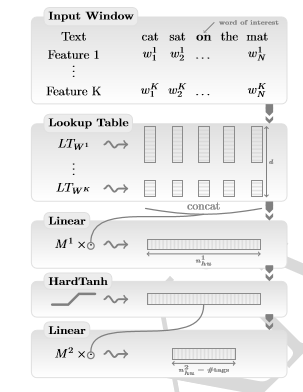
\includegraphics[width=\textwidth]{translations/f1.png}
\caption*{图一\ 单词方法的神经网络结构 \label{translation_f1}}
\end{center}
\end{figure}

\begin{figure}[!hbp]
\begin{center}
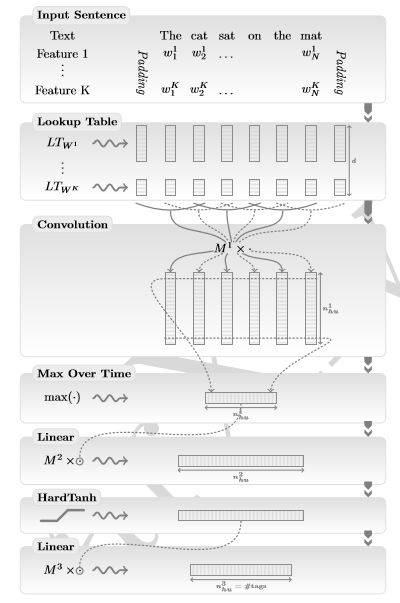
\includegraphics[width=\textwidth]{translations/f2.png}
\caption*{图二\ 句子方法的神经网络结构 \label{translation_f2}}
\end{center}
\end{figure}
\subsection*{3.1  将单词转化为特征向量}
我们结构的一个要点就是它在(几乎是)直接使用单词时也能发挥地很好。因此,对于我们的方法来说,学习到一个好的词语表达方式是非常重要的。为了保证效率,单词以在一个有限词典$D$中的序号的方式输入我们的结构。很明显,简单的序号并没有携带太多有用的信息。不过,网络的第一层通过查表操作将序号映射到一个特征向量上。在赋予了具体任务之后,每个单词的相关表示都能通过向后传播训练在对应的查找表格中找到。
正式来说,对于每个单词$w \in D$,通过查表层$LT_W(\cdot)$会赋予一个$d_{wrd}$维内部特征向量:
$$
LT_W(w) = {\left \langle W \right \rangle }^1_w
$$
此处,$W \in {\mathbb{R}}^{d_{wrd} \times |D|}$是需要被学习的参数矩阵,${\left \langle W \right \rangle}_w^1 \in {\mathbb{R}}^{d_{wrd}}$是W的第i列,而$d_{wrd}$是单词向量的长度(需要被用户选择的超参数)。
输入一句话或者长度为$T$的单词序列$[w]^T_1$,其中单词都存在于词典$D$中,则查表层会对序列中所有单词同样的操作,产生以下输出矩阵:
$$
LT_W([W]^T_1)=({\left \langle W \right \rangle }^1_{[w]_1}, {\left \langle W \right \rangle }^1_{[w]_2} ... {\left \langle W \right \rangle }^1_{[w]_r}) \eqno{1}
$$
该矩阵可以被应用于之后的神经网络层,我们在下文中将介绍。

\subsubsection*{3.1.1 拓展到任意离散特征}
当研究者们认为单词以外的特征对特定任务有帮助时,他们可能需要向神经网络输入这些特征。例如,在命名实体识别任务中,可能需要提供词语是否存在于地名词典中的特征。另外一个常见情况是需要引入一些基本的预处理,比如词干化或者需要处理大小写问题。在这种情况中,单词可能被三个离散特征代表:小写字母形式的词干,小写字母形式的结尾,首字母大写形式的词汇本身。
总的来说,我们可以假设词汇w被$K$个离散特征表示,此处$w \in D^1 \times ... \times D^K$, $D^k$代表第k个特征的词典。我们可以将每个特征与一个查找表$LT_{w^k}(\cdot)$关联起来,此处参数$W^k \in {\mathbb{R}}^{d_{wrd}^k \times |D_k|}$,$d_{wrd}^k \in \mathbb{N}$是用户定义的特征向量维度。对于单词w来说,特征向量维度为$d_{wrd}=\sum_k{d_{wrd}^k}$,由所有查找表的输出连接而成。
$$
LT_{W^1,...,W^K}(w) = \begin{pmatrix}
\\ LT_{W^1}(w_1)
\\. 
\\.
\\.
\\ LT_{W^K}(w_K)
\end{pmatrix} =
\begin{pmatrix}
\\ {\left \langle W^1 \right \rangle}^1_{w_1}
\\. 
\\.
\\.
\\ {\left \langle W^K \right \rangle}^1_{w_K}
\end{pmatrix}
$$
查找表的输出矩阵与(16)类似,但每个离散特征为其添加了额外的行:
$$
LT_{W^1,...,W^K}(|W|^T_1) = 
\begin{pmatrix}
\\{\left \langle W^1 \right \rangle}^1_{[W_1]_1} ... {\left \langle W^1 \right \rangle}^1_{[W_1]_T}
\\.
\\.
\\.
\\{\left \langle W^K \right \rangle}^1_{[W_K]_1} ... {\left \langle W^K \right \rangle}^1_{[W_K]_T}
\end{pmatrix} \eqno{2}
$$
这些查找表内的特征向量有效地学习了词典中词汇的特征。现在,我们可以将这些可训练的特征输入更深层次的可训练特征抽取流程,如此就可以表示词组,最终,表示整个句子。

\subsection*{3.2 从词汇特征向量中抽取高层次的特征向量}
查找表层产生的特征向量需要在后续神经网络层中被组合,以此决策句子中的每个单词的标签。为可变长序列中的元素产生标签(这里,句子是一个单词序列)是机器学习中的标准问题。我们提出了两种每次标注一个单词的通用方式:窗口方法和(基于卷积的)句子方法。

\subsubsection*{3.2.1 窗口方法}
窗口方法假设单词的标签主要依赖于它周围的单词。给定一个需要标注标签的单词,我们通常考虑从其周围$k_{sz}$(给定值,超参数)大小的单词窗口。所有在这个窗口内的单词都首先被传进查表层(16)或者(2),以产生大小为固定值$d_{wrd} \times k_{sz}$的单词特征矩阵。可以将该矩阵每列相连接,则此时该矩阵可以被视为$d_{wrd}k_{sz}$维的向量。正式地说,第一层网络输出的词窗口特征向量可以被写为:
$$
f_0^1 = {\left \langle LT_w({[w]_1^T})\right \rangle}_t^{d_{win}} = 
\begin{pmatrix}
\\{\left \langle W \right \rangle}^1_{{[w]}_{t-d_{win}/2}}
\\.
\\.
\\.
\\{\left \langle W \right \rangle}^1_{{[w]}_{t}}
\\.
\\.
\\.
\\{\left \langle W \right \rangle}^1_{{[w]}_{t+d_{win}/2}}
\end{pmatrix} \eqno{3}
$$

\paragraph*{线性层}
固定维度的向量$f_0^1$可以作为一层或多层标准神经网络层的输入,这些层为输入提供了几何映射:
$$
f_{\theta}^l=W_lf_{\theta}^{l-1} + b^l \eqno{4}
$$
这里$W^l \in {\mathbb{R}}^{n^{t}_{hu} \times n^{t-1}_{hu}},b^l \in {\mathbb{R}}^{n^{t}_{hu}}$都是需要被训练的参数,$n_{hu}^l$是超参数,代表第l层隐藏单元的数目。

\paragraph*{HardTanh层}
多层线性神经网络通常是被堆叠在一起的,使用非线性函数交织在一起,以抽取出高层的非线性的特征。如果没有引入非线性函数,那么我们的模型就将只是简单的线性模型。我们使用了双曲正切函数的“硬”版本作为非线性函数,它具有计算代价稍低的特点(与原本的双曲正切函数相比),同时能保持泛化表现不变(Collobert, 2004)。第l层在输入向量上应用HardTanh函数:
$$
{[f^l_{\theta}]}_i = HardTanh([f^{l-1}_{\theta}]),
$$
此处
$$
HardTanh(x) = \left\{\begin{matrix}
-1 & if\ x<-1 \\ 
x & if\ -1<=x<=1\\ 
1 & if\ x > 1 
\end{matrix} \right. \eqno{5}
$$

\paragraph*{打分}
最终,网络最后一层L的输出向量维数将会与相关任务的标签数目一致。每个输出之后都能被翻译为对应标签的分数(需要知道网络输入信息),这主要是因为我们仔细挑选了一个代价函数,该函数将在下面的章节介绍。

\paragraph*{备注1(边际效应)}
特征窗口没有很好地定义如何处理开头或者结尾处的单词。为了智慧地解决这个问题,我们使用了一个特殊的单词"PADDING"(填充)在句子首尾复制$d_{win}/2$次。这与使用"start"(开始)和"end"(结束)符号的方法本质上是一致的。

\subsection*{3.2.2 句子方法}
在实验结果分析章节我们将会发现仅仅只用窗口方法就能够解决大多数我们感兴趣的问题。但是,该方法难以解决语义角色标注问题。在该问题中某个词语的标签取决于在这个句子中位置比该词语更靠前的动词(更正式的说法是谓语)。如果该动词落在词语窗口之外,系统就不能够正确地分类该词语。在这种特殊情况下,分类这个词需要考虑整个句子。当使用神经网络时,我们可以自然地想到能够使用卷积神经网络解决该问题。该想法首先为Waibel等所提出(1989),在文献中被称作时延神经网络(Time Delay Neural Networks, TDNNs)。
我们会在接下来详细介绍卷积神经网络。它将整个句子连续输入,经过查表层(16),由卷积层在句中每个单词周围产生局部特征,将这些局部特征结合在一起可以生成全局特征向量,该向量可以输入标准的仿射层(4)。在语义角色标注的例子中,该操作在句子中的每个词语上,每个动词上执行。因此,在神经网络中标注希望纳入考虑的是哪个动词,希望进行标注的是哪个词语是非常重要的。为了这个目的,位置i上的词语会增加两个如3.1.1描述的特征,这些特征描述了两个相对距离$i-pos_v$和$i-pos_w$,此处被选择的动词在$pos_v$位置上,要被标注的单词在$pos_w$位置上。

\paragraph*{卷积层}
卷积层可以被视为窗口方法的一种泛化:给定一个由矩阵$f_{\theta}^{l - 1}$的若干列表示的序列(在查找表中(1)),(4)中的由矩阵转化为向量的操作在序列中连续的每个窗口内执行,用之前的记号,第l层输出第t列可以被计算为:
$$
{\left \langle {f_{\theta}^{l}}\right \rangle}^1_t = W^l{\left \langle {f_{\theta}^{l - 1}}\right \rangle}^{d_{win}}_t + b^l, \forall{t} \eqno{6}
$$
此处权重矩阵$W^l$在整个序列的所有窗口计算时保持不变。卷积层抽取给定序列每个窗口内的局部特征。为了输出给标准仿射层(4),若干卷积层通常被堆叠在一起以获取高层次的特征。在这种情况下,每层后面一定要使用非线性函数(5),否则整个卷积网络就相当于一层卷积网络。

\paragraph*{最大层}
输出(6)的大小取决于输入神经网络的句子的大小。被卷积神经网络抽取的局部特征向量需要被结合为全局特征向量,该向量需要有一个固定的,与句子长度无关的维数,以便于输入接下来的标准仿射层。传统卷积神经网络往往在序列(6)的时间t上使用计算平均值(计算时可能带有权重)或者最大值的方式完成这一点。(这里“时间”只代表其在句子中的位置,该术语来源于卷积神经网络的某些应用方式,例如语音数据,该数据为时间序列。)在我们的研究中,平均值没有很大意义。另外,通常来说大部分词语对给定词的语义角色标注都没有什么影响,因此,我们使用最大值方法,它迫使神经网络获取卷积层产生的最有用的局部特征(如图3所示)。设卷积层l-1的输出为矩阵$f_{\theta}^{l - 1}$,则最大层l的输出为向量$f_{\theta}^l$:
$$
{[f_{\theta}^l]}_i = \max_t{{f_{\theta}^{l-1}}_{i,t}} \ 1<=i<=n_{hu}^{t-1} \eqno{7}
$$
该定长全局特征随后可以输入标准仿射层(4)。如窗口方法一样,我们最终可以为每个可能的标签进行打分。

\subsection*{3.1  将单词转化为特征向量}

\begin{figure}[!hbp]
\begin{center}
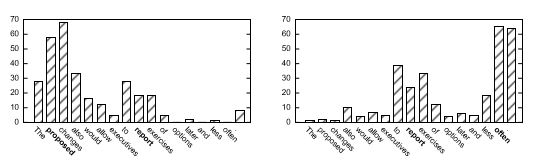
\includegraphics[width=\textwidth]{translations/f3.png}
\caption*{图三\ 每个词汇被最大层挑选的特征数量 \label{translation_f3}}
\end{center}
这张图片中我们考虑的是为了训练语义角色标注的图2中语句方法的神经网络。卷积神经网络产生的“局部”特征是每个单词300维,在使用过最大层后,我们得到了整个语句的300维特征。可以发现神经网络比较倾向与注意相关的动词(如"report")和词语(如"proposed"(左图),"often"(右图))
\end{figure}

\paragraph*{备注 2}
在卷积神经网络(6)中也有类似窗口方法(3)的边际效应,我们再次使用为句子填充特殊单词的方法解决这个问题。

\subsubsection*{3.2.3 标注方案}
如前述,神经网络输出层为当前任务的所有可能标签打分。在窗口方法中,这些标签对应于窗口正中心的词语,但在句子方法中,这些标签对应于网络输入中额外标记的单词。
词性标注任务实际上标注了每个词语的句法角色。剩下的三个任务的标签则主要依赖句子的一段。这三个任务通常用特殊的标注方案,如表3所示,以识别句子的段落。有些这样的方案已经被学者充分定义了(如IOB, IOE, IOBES,...),目前对于哪个方案更好还没有统一结论。最好的表现成果有时是通过结合通过不同标注方案训练的分类器获得的。
命名实体识别,分块和语义角色标注任务目前都使用了两种不同的标注方案。为了消除这个额外资源所带来的变化,我们决定所有任务中都使用最具有表达力的IOBES标注方案。举例来说,在分块任务中,我们用四种不同的标签来描述名词。标签"S-NP"用于描述只包含一个词语的名词短语。标签"B-NP","I-NP","E-NP"则分别描述具有多个词语的名词短语的第一个,中间和最后一个词语。还有一个额外的标签"O"用来表示这个单词不在分块之中。在测试时,这些标签又被转化为原本的IOB标签方案以便输入如2.5小节提到的标准性能评估阶段。

\begin{figure}[!hbp]
\begin{center}
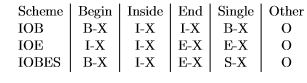
\includegraphics[width=\textwidth]{translations/f4.png}
\caption*{表三\ 不同的标注方案 \label{translation_f4}}
\end{center}
在分块中每个标注中存在"X"的单词都会根据位置(开头,中间,结尾)被标注上它的前缀。单独一个词语的分块也在输出中。不在已标注分块中的单词被标为"O"。IOB(和IOE)方案有一些变化,这里将不和其它带有"X"的分块邻接的分块前缀中"B"或者"E"替代为"I"。
\end{figure}

\subsection*{3.3 训练}
所有神经网络都通过使用随机梯度下降算法最大化训练数据的整体似然计算得到。如果我们令$\theta$为神经网络中所有可训练参数的代称,当用训练集$\mathbb{T}$训练时,我们希望最大化以下与$\theta$有关的似然:
$$
\theta \rightarrow \sum_{(x,y) \in \mathbb{T}}{\log{p(y|x, \theta)}} \eqno{8}
$$
这里x为一个训练词语窗口或者句子以及其相关的特征,y代表与之相关的正确标签。概率$p(\cdot)$由神经网络的输出与标签计算而来。我们会在接下来的部分看到如何将神经网络的输出转化为概率。

\subsubsection*{3.3.1 单词层级的似然对数值}
在这种方法中,句子中的每个单词都被认为是独立的。给定输入样例为x,则参数为$\theta$的神经网络输出的对于第i个标签的分数为${[f_{\theta}(x)]}_i$。为了简化该记号,我们先去除x的影响,只考虑${[f_{\theta}]}_i$。则分数可以通过在所有可用标签上执行softmax操作而被转化为标签的条件概率$p(i|x,\theta)$:
$$
p(i|x, \theta) = \frac{e^{{[f_{\theta}]}_i}}{\sum_i{e^{{[f_{\theta}]}_i}}} \eqno{9}
$$
定义操作log-add为:
$$
\mathop{logadd}_iz_i = log(\sum_i e^{zi}) \eqno{11}
$$
如此,我们就能够像这样表达某个训练样本$(x,y)$的似然对数值:
$$
\log p(y|x, \theta) = {[f_{\theta}]}_y - \mathop{logadd}_j{[f_{\theta}]}_j \eqno{11}
$$
该训练公式通常又被视为交叉熵,其被广泛地应用在分类问题中。在我们的例子中它也许不是最好的,因为通常句子中的某个词语的标签和周围单词的标签有某种联系。在接下来的章节我们将介绍另一个神经网络常用的计算方法,这种方法注重一个句子中被预测出的标签之间的依赖关系。

\subsubsection*{3.3.2 语句层级的似然对数值}
在类似于分块,命名实体识别,语义角色标注的任务中,我们知道在语句中的标签彼此存在依赖关系:有些标签主要与分块有关,有些则不应该被另外一些标签影响。我们考虑了一种将句子结构纳入考虑的训练方案:当给定神经网络对某个句子中所有单词的标签预测,且给定标签转移的分数,我们希望能鼓励一些标签转化的路径生成,同时抑制另外一些路径。
考虑神经网络的分数矩阵$f_{\theta}({[x]}_1^{\mathbb{T}})$,像前一个章节的方法一样,为了简化符号,我们暂时不考虑输入${[x]}_1^{\mathbb{T}}$的影响。则${[f_{\theta}]}_{i,t}$为在语句${[x]}_1^{\mathbb{T}}$对应第i个单词,第i个标签,且参数为${\theta}$的分数输出。
在此我们提出转移分数这个概念,${[A]}_{i,j}$代表在连续的单词中从标签i转移到标签j的分数。${[A]}_{i,0}$则代表从第i个标签开始的分数。由于转移分数矩阵与${\theta}$类似,也是要被训练的参数之一,我们定义$\tilde{\theta} = \theta \cup {\{{[A]}_{i,j}\ \forall i, j\}}$。则语句${[x]}_1^{\mathbb{T}}$沿着路径${[i]}_1^{\mathbb{T}}$的分数可由转移分数和网络输出分数之和给出:
$$
s({[x]}_1^{\mathbb{T}}, {[i]}_1^{\mathbb{T}}, \tilde{\theta}) = \sum^{\mathbb{T}}_{t=1}({[A]}_{{[i ]}_{t - 1}, {[i ]}_{t}} + {[f_{\theta}]}_{{[i]_t}, t}) \eqno{12}
$$
与词语层级的似然值(11)很相近,在词语层级我们使用softmax(9)归一化所有标签,在语句层级我们也使用softmax归一化所有可能的标签路径${[j]}^{\mathbb{T}}_1$,然后我们将结果比值转化为标签路径的条件概率。在对数操作后,真正的路径${[y]}_1^{\mathbb{T}}$的条件概率为:
$$
\log{p({[y]}_1^{\mathbb{T}}| {[x]}_1^{\mathbb{T}}, \tilde{\theta})} = s({[x]}_1^{\mathbb{T}}, {[i]}_1^{\mathbb{T}}, \tilde{\theta}) - \mathop{logadd}_{\forall {[j]}_1^{\mathbb{T}}}\ {s({[x]}_1^{\mathbb{T}}, {[i]}_1^{\mathbb{T}}, \tilde{\theta})} \eqno{13}
$$  
由于logadd操作(11)中的短语个数与标签个数相同,所以在(13)中它随句子的长度指数性增长。幸运的是,利用在半环($\mathbb{R} \cup \{-{\infty}\}, logadd, +$)上的结合律和分布律,我们可以重复以下关于t的标准迭代在线性时间计算出结果:
$$
\begin{matrix}
{\delta}_t(k) & \triangleq \mathop{logadd}_{{[j]}^t_1 \cap {[j]}_t = k} s({[x]}_1^{t}, {[i]}_1^{t}, \tilde{\theta}) \\
& = \mathop{logadd}_i{\ \mathop{logadd}_{{[j]}^t_1 \cap {[j]}_{t-1} = i \cap {[j]_t = k}}} s({[x]}_1^{t}, {[j]}_1^{t-1}, \tilde{\theta}) + {[A]}_{{[j]}_{t-1,k}} + {[f_{\theta}]}_{k, t}\\
& = \mathop{logadd}_{i}{\  {\delta}_{t - 1}(i)} + {[A]}_{i,k} + {[f_{\theta}]}_{k,t}\\
& = {[f_{\theta}]}_{k,t} + \mathop{logadd}_{i}{\  ({\delta}_{t - 1}(i) + {[A]}_{i, k})}, \forall k, 
\end{matrix} \eqno{14}
$$
终止条件为:
$$
\mathop{logadd}_{\forall {[j]}_1^{\mathbb{T}}} s({[x]}_1^{\mathbb{T}}, {[i]}_1^{\mathbb{T}}, \tilde{\theta}) = \mathop{logadd}_i{\ \delta_{\mathbb{T}}(i)} \eqno{15}
$$
我们现在可以在所有训练样本对$({[x]}_1^{\mathbb{T}}, {[y]}_1^{\mathbb{T}})$对(8)中最大化似然值(13)。
在推测阶段,对于给定的语句${[x]}_1^{\mathbb{T}}$,我们需要找到最好的标签路径,以最小化语句分值(12),也就是说我们必须找到:
$$
\mathop{argmax}_{{[y]}_1^{\mathbb{T}}}s({[x]}_1^{\mathbb{T}}, {[i]}_1^{\mathbb{T}}, \tilde{\theta})\eqno{16}
$$
此时使用Viterbi算法是非常自然的选择,因为它相当于每步都在迭代(14)和(15),不过在Viterbi算法中logadd被max所代替,最后通过每个max找回最优路径。


\newpage
\section*{外文译文原文}
\begin{center}
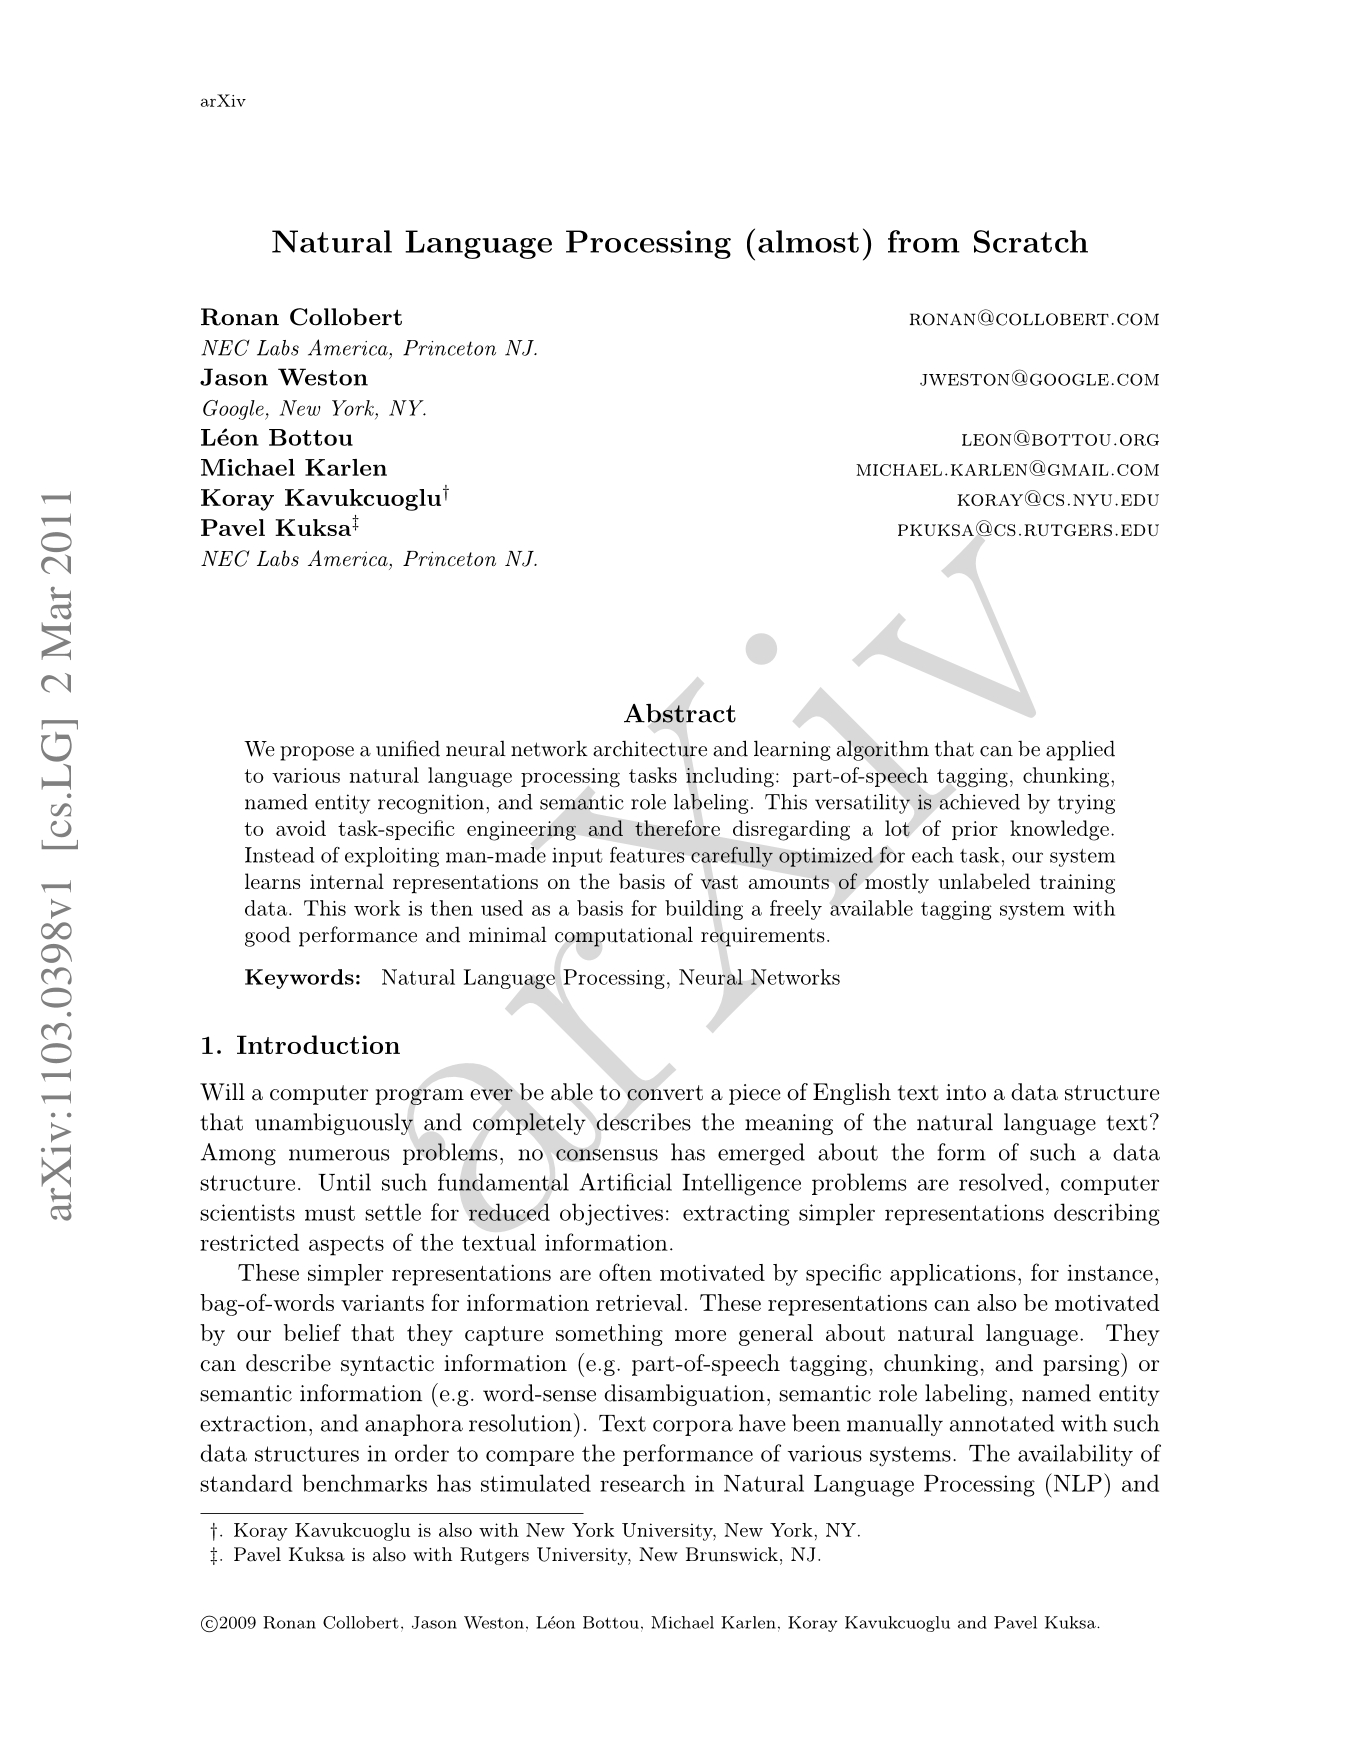
\includegraphics[width=\textwidth]{translations/collobert_2011-1.jpg}
\end{center}
\begin{center}
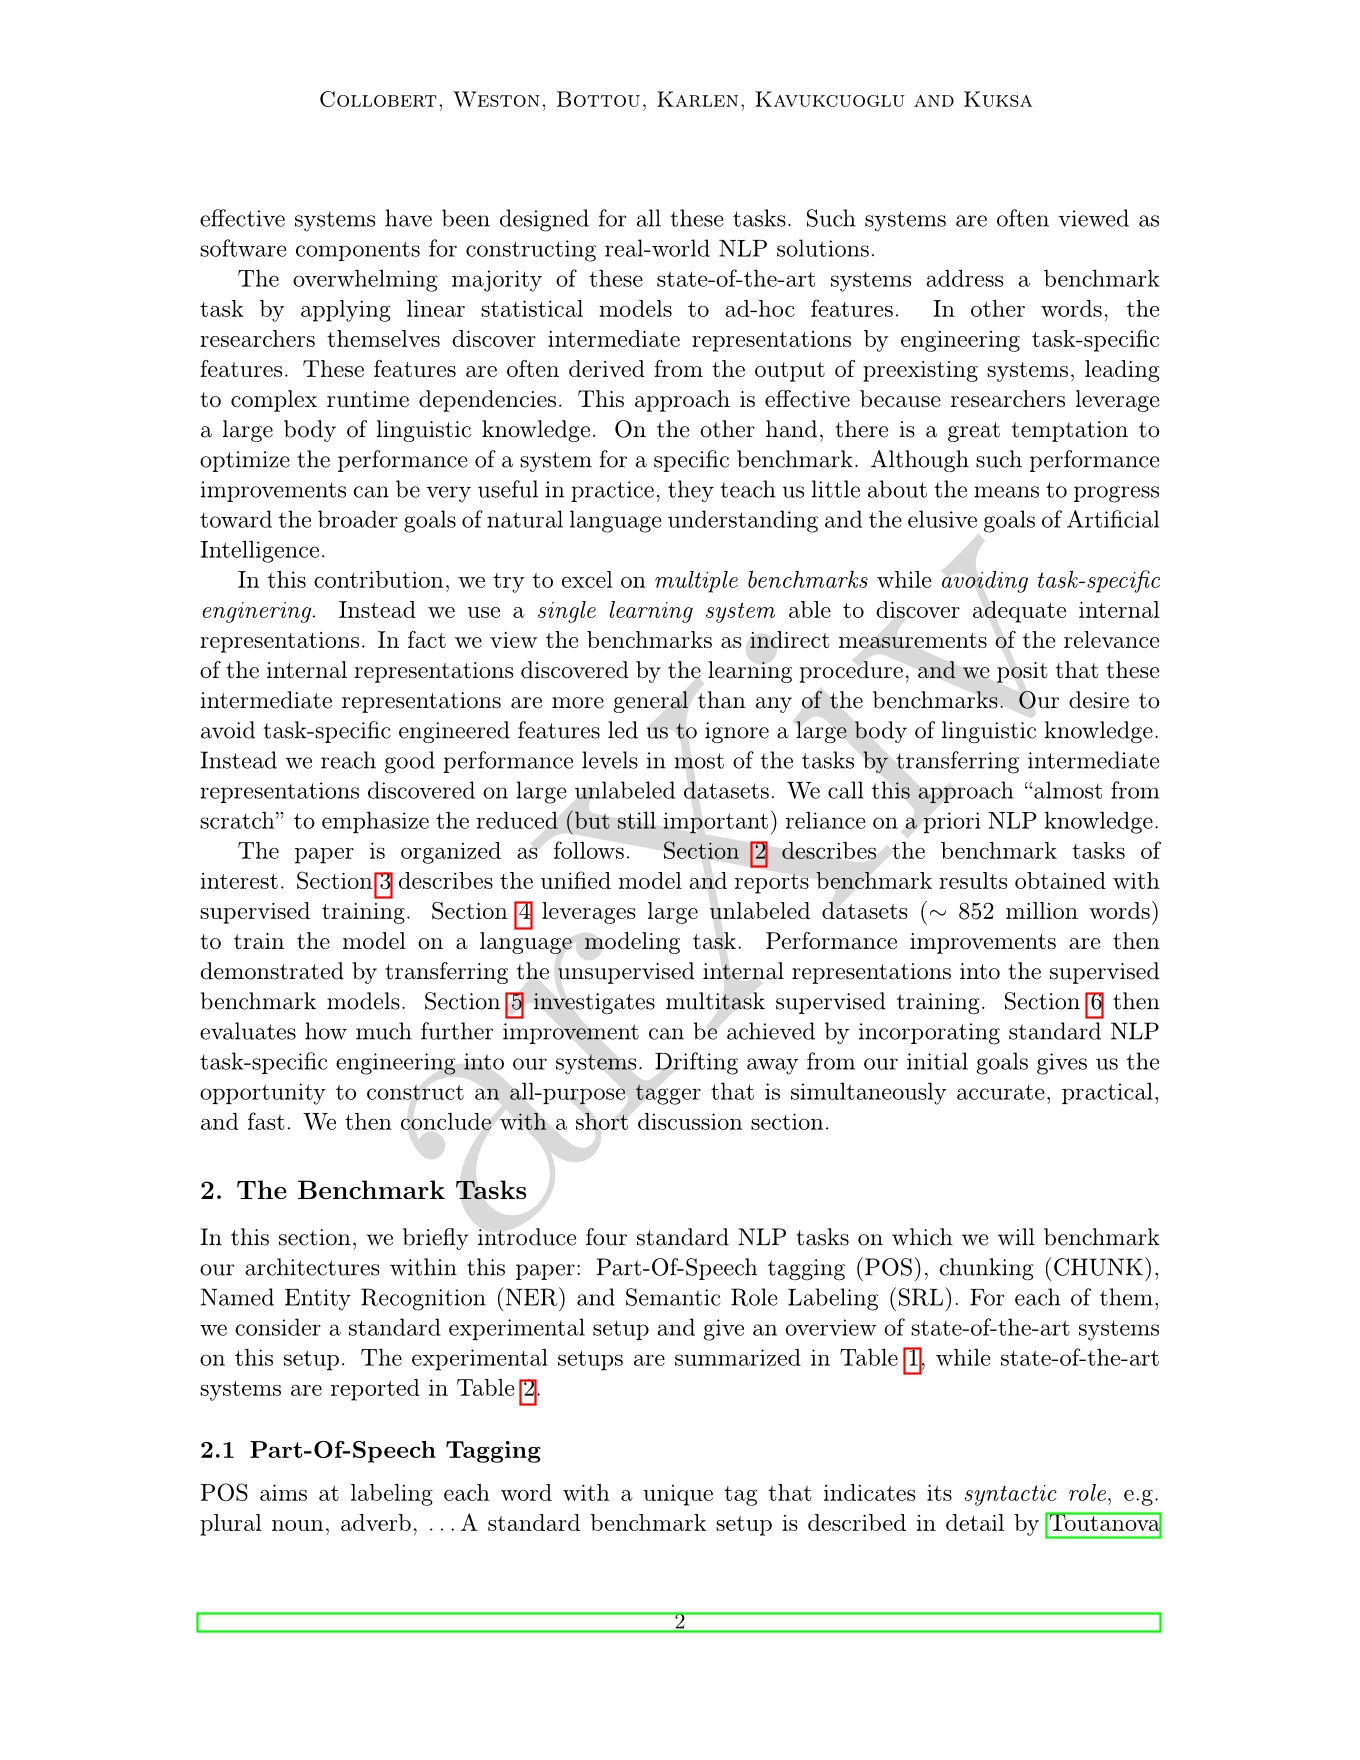
\includegraphics[width=\textwidth]{translations/collobert_2011-2.jpg}
\end{center}
\begin{center}
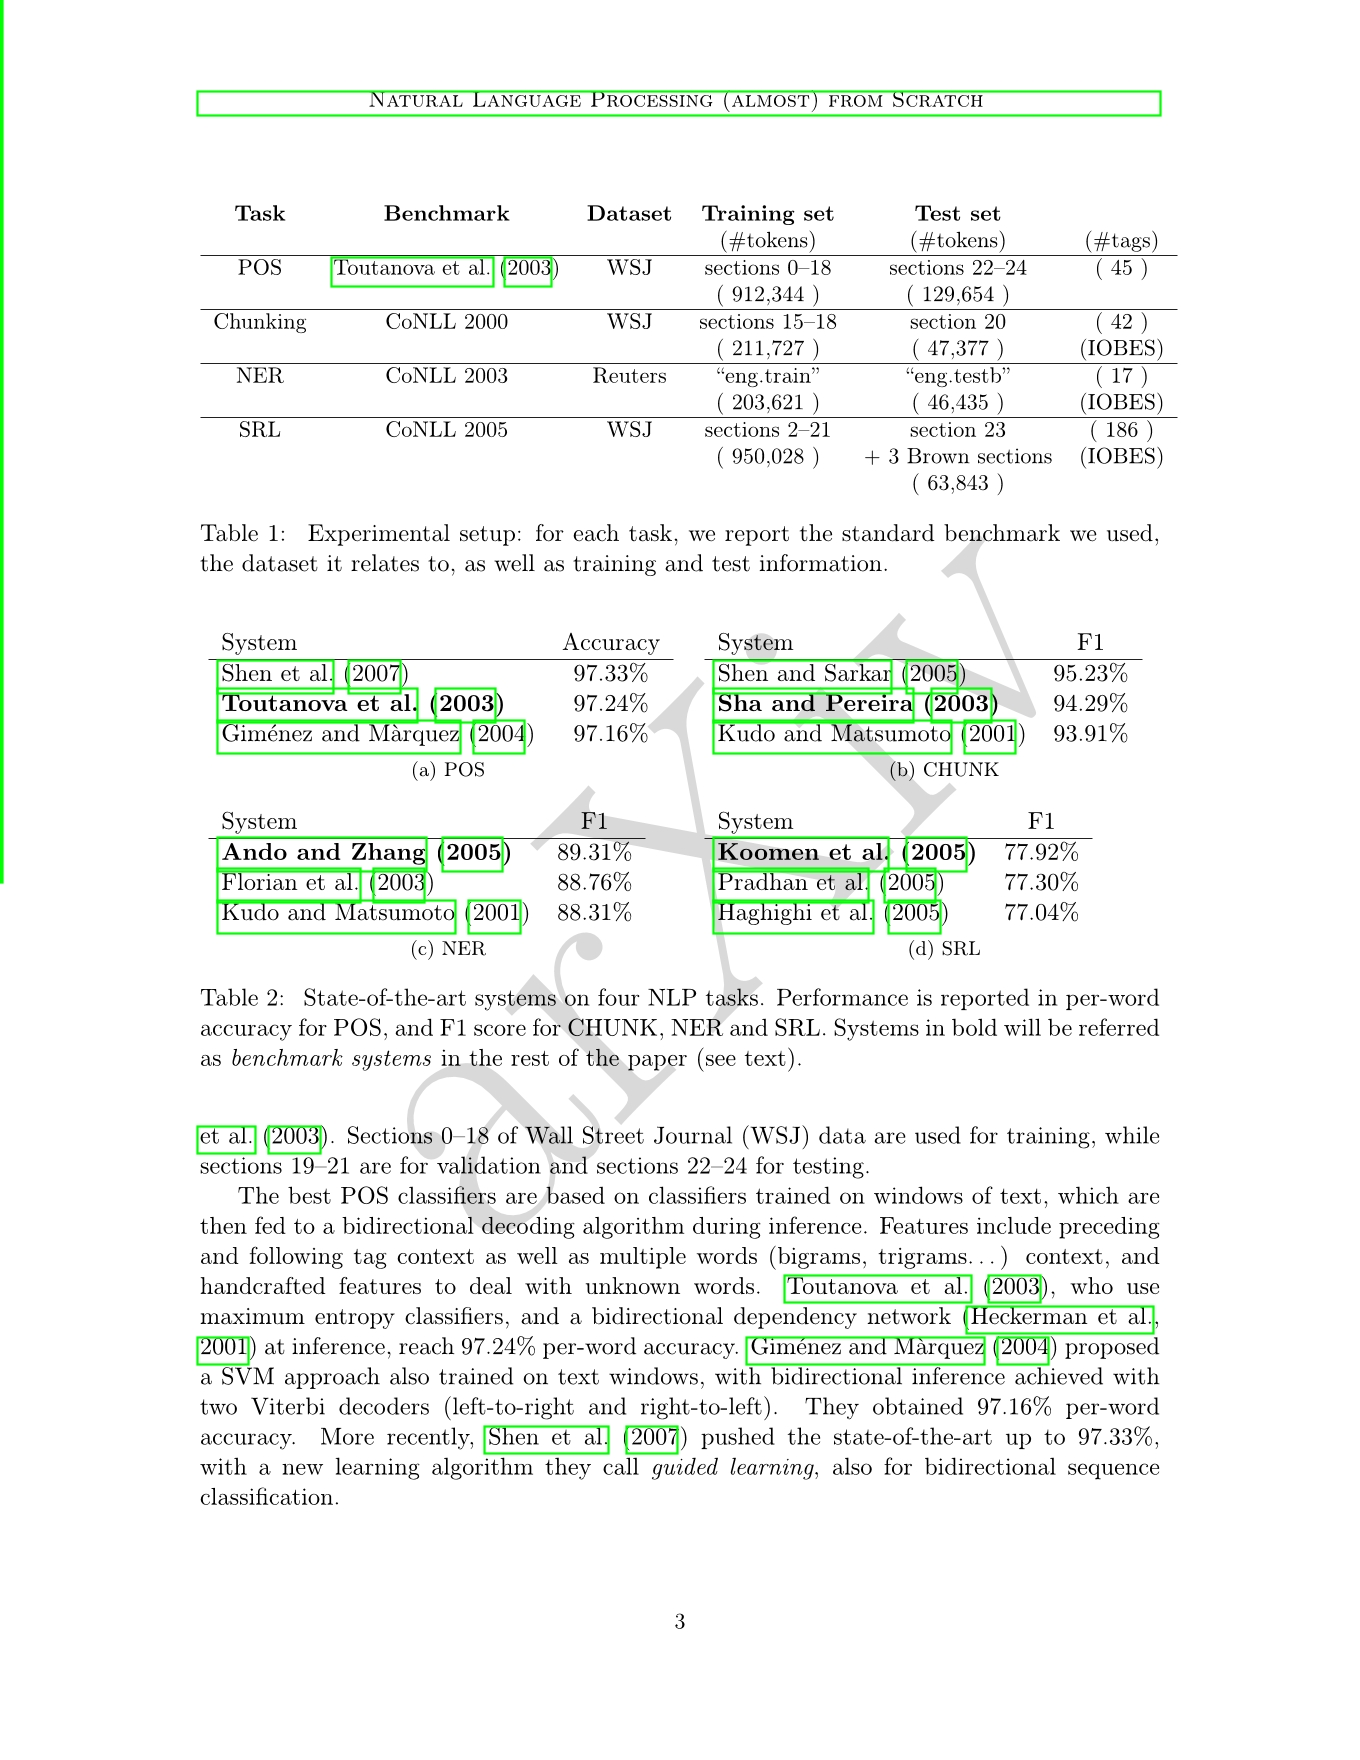
\includegraphics[width=\textwidth]{translations/collobert_2011-3.jpg}
\end{center}
\begin{center}
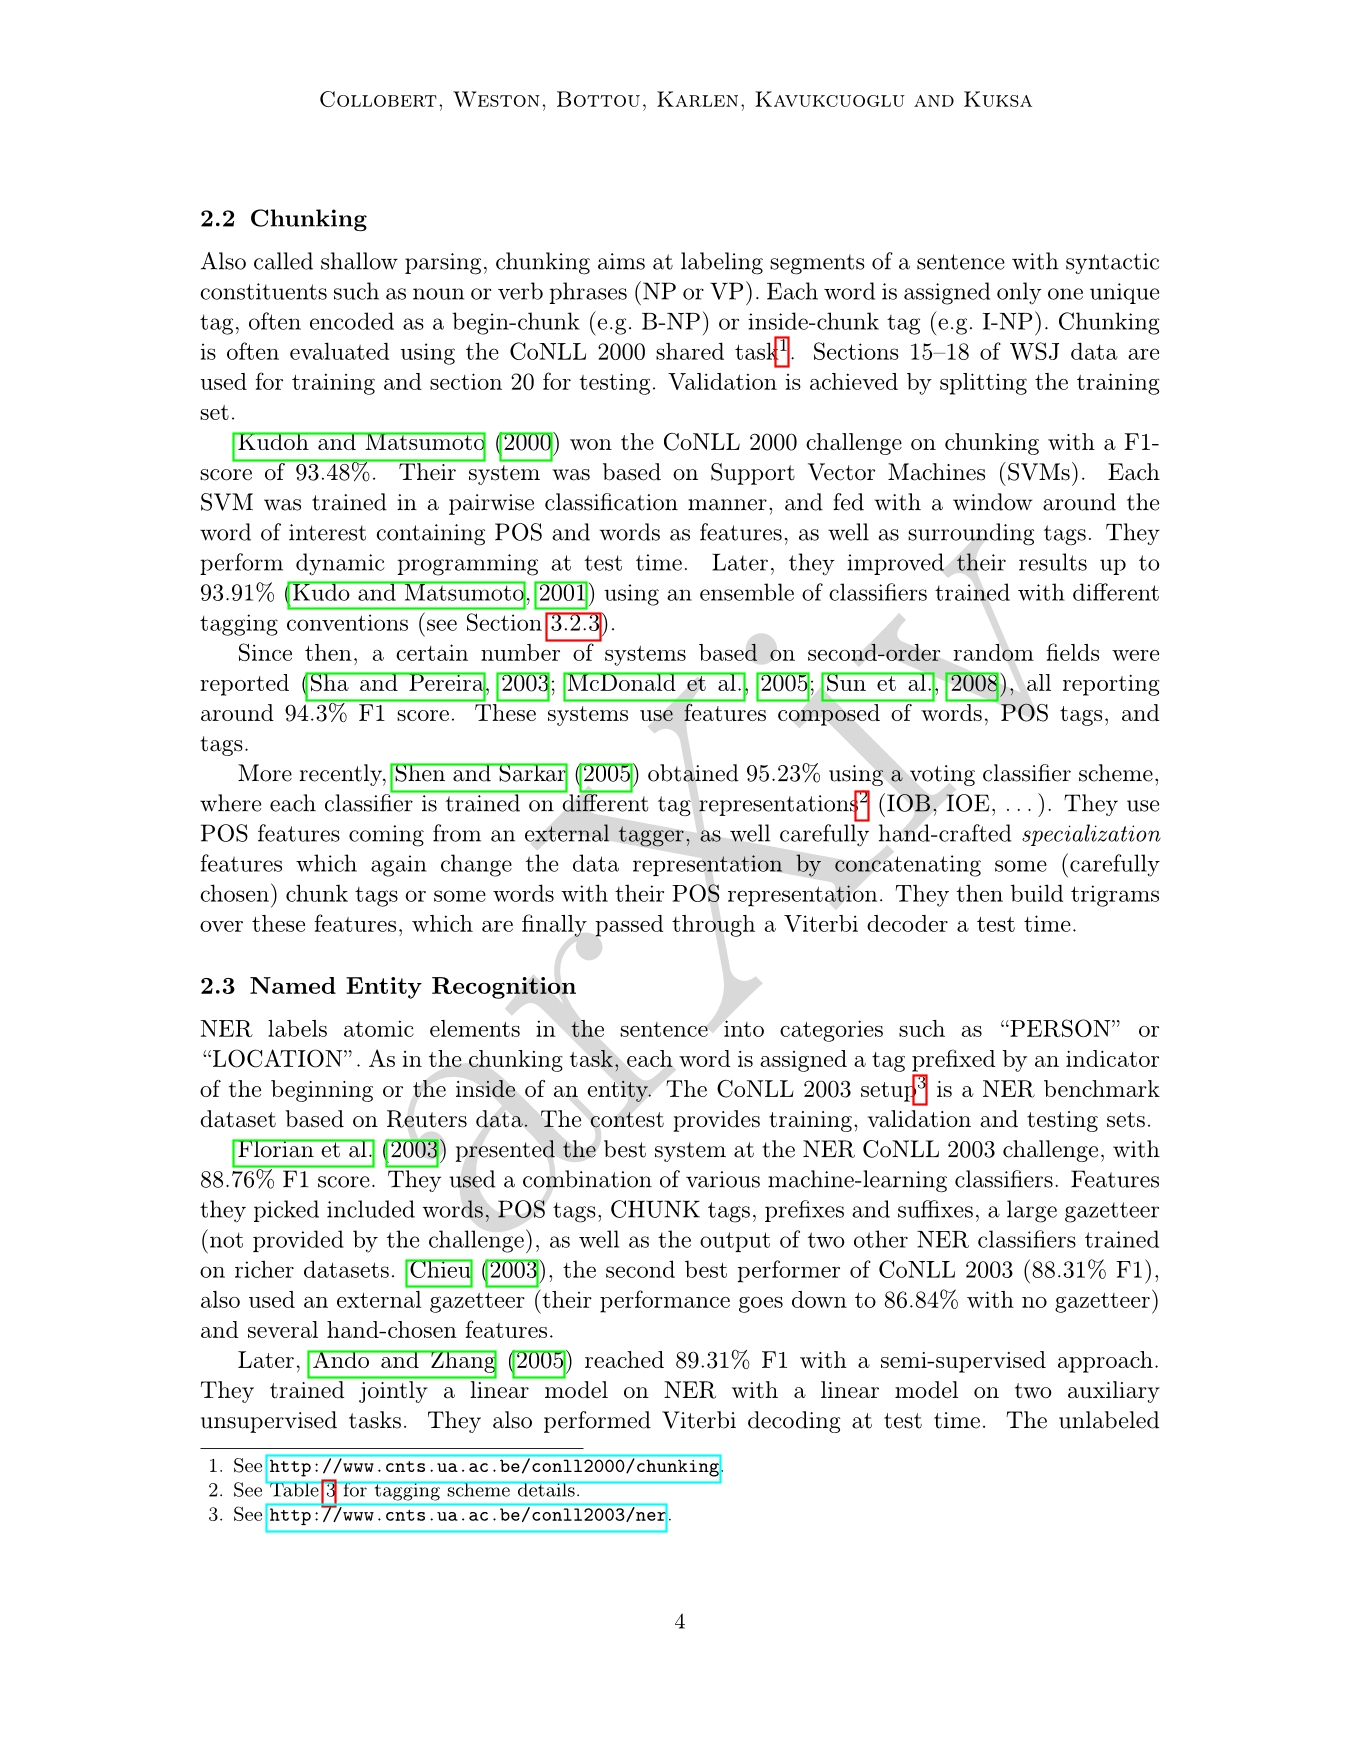
\includegraphics[width=\textwidth]{translations/collobert_2011-4.jpg}
\end{center}
\begin{center}
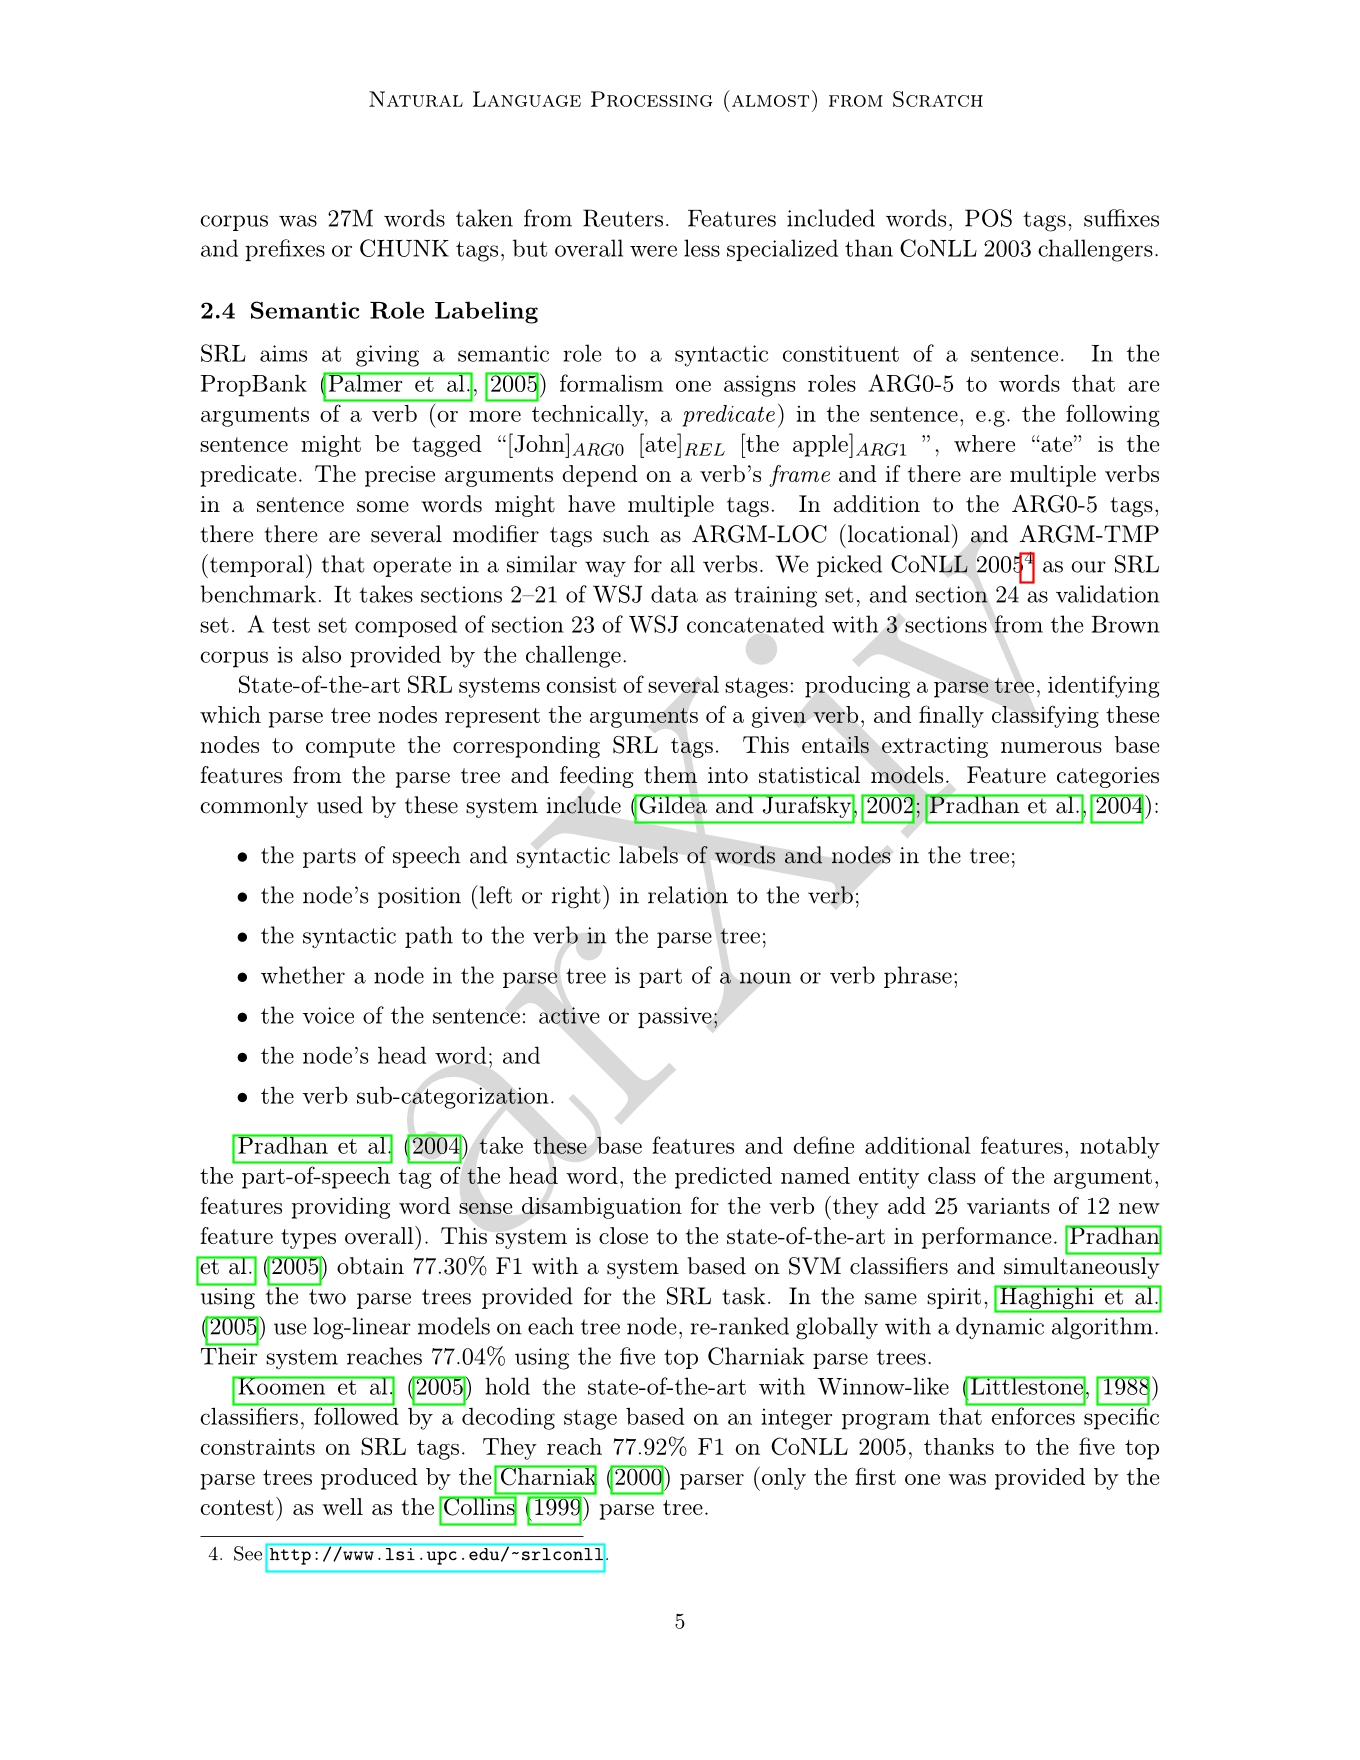
\includegraphics[width=\textwidth]{translations/collobert_2011-5.jpg}
\end{center}
\begin{center}
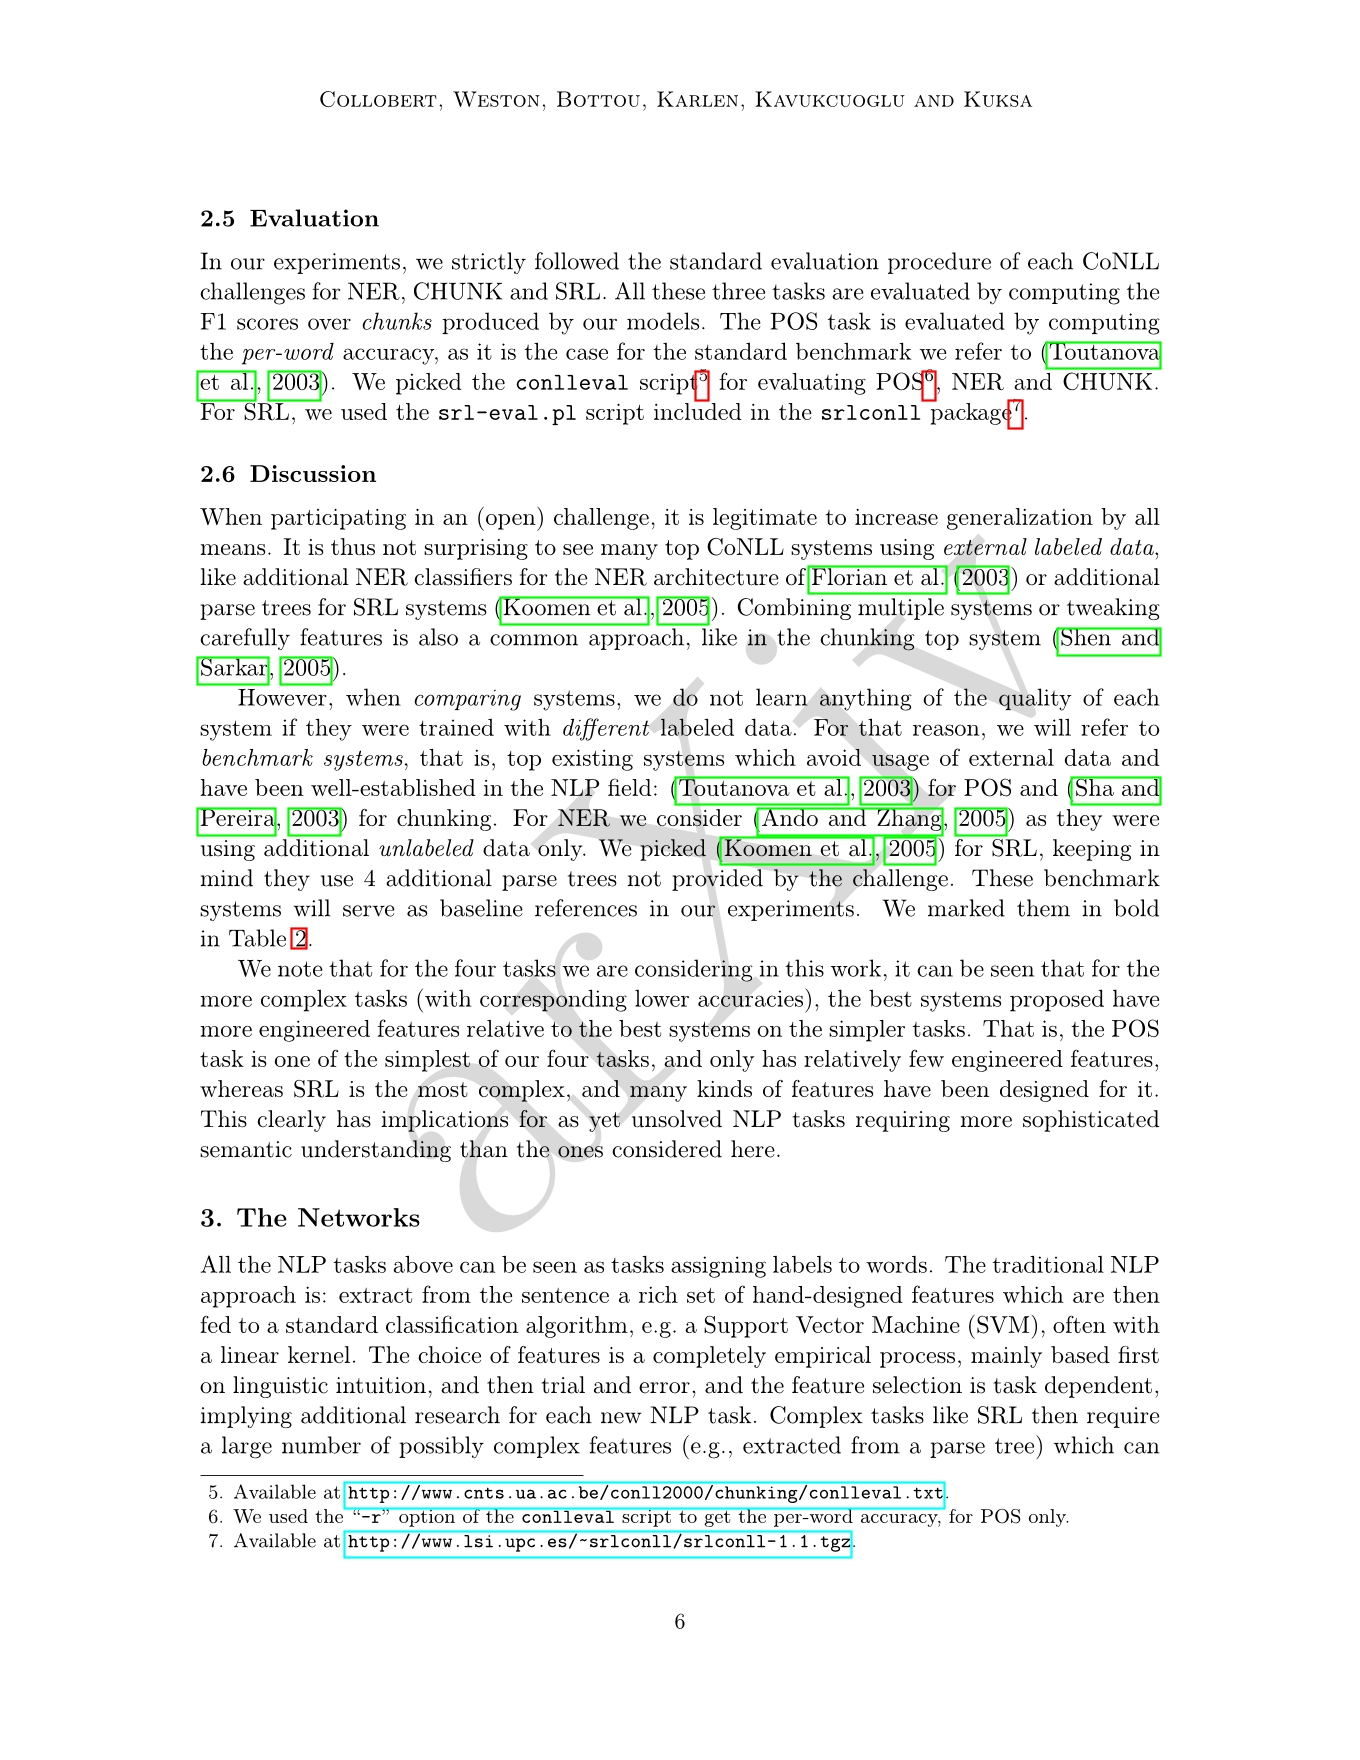
\includegraphics[width=\textwidth]{translations/collobert_2011-6.jpg}
\end{center}
\begin{center}
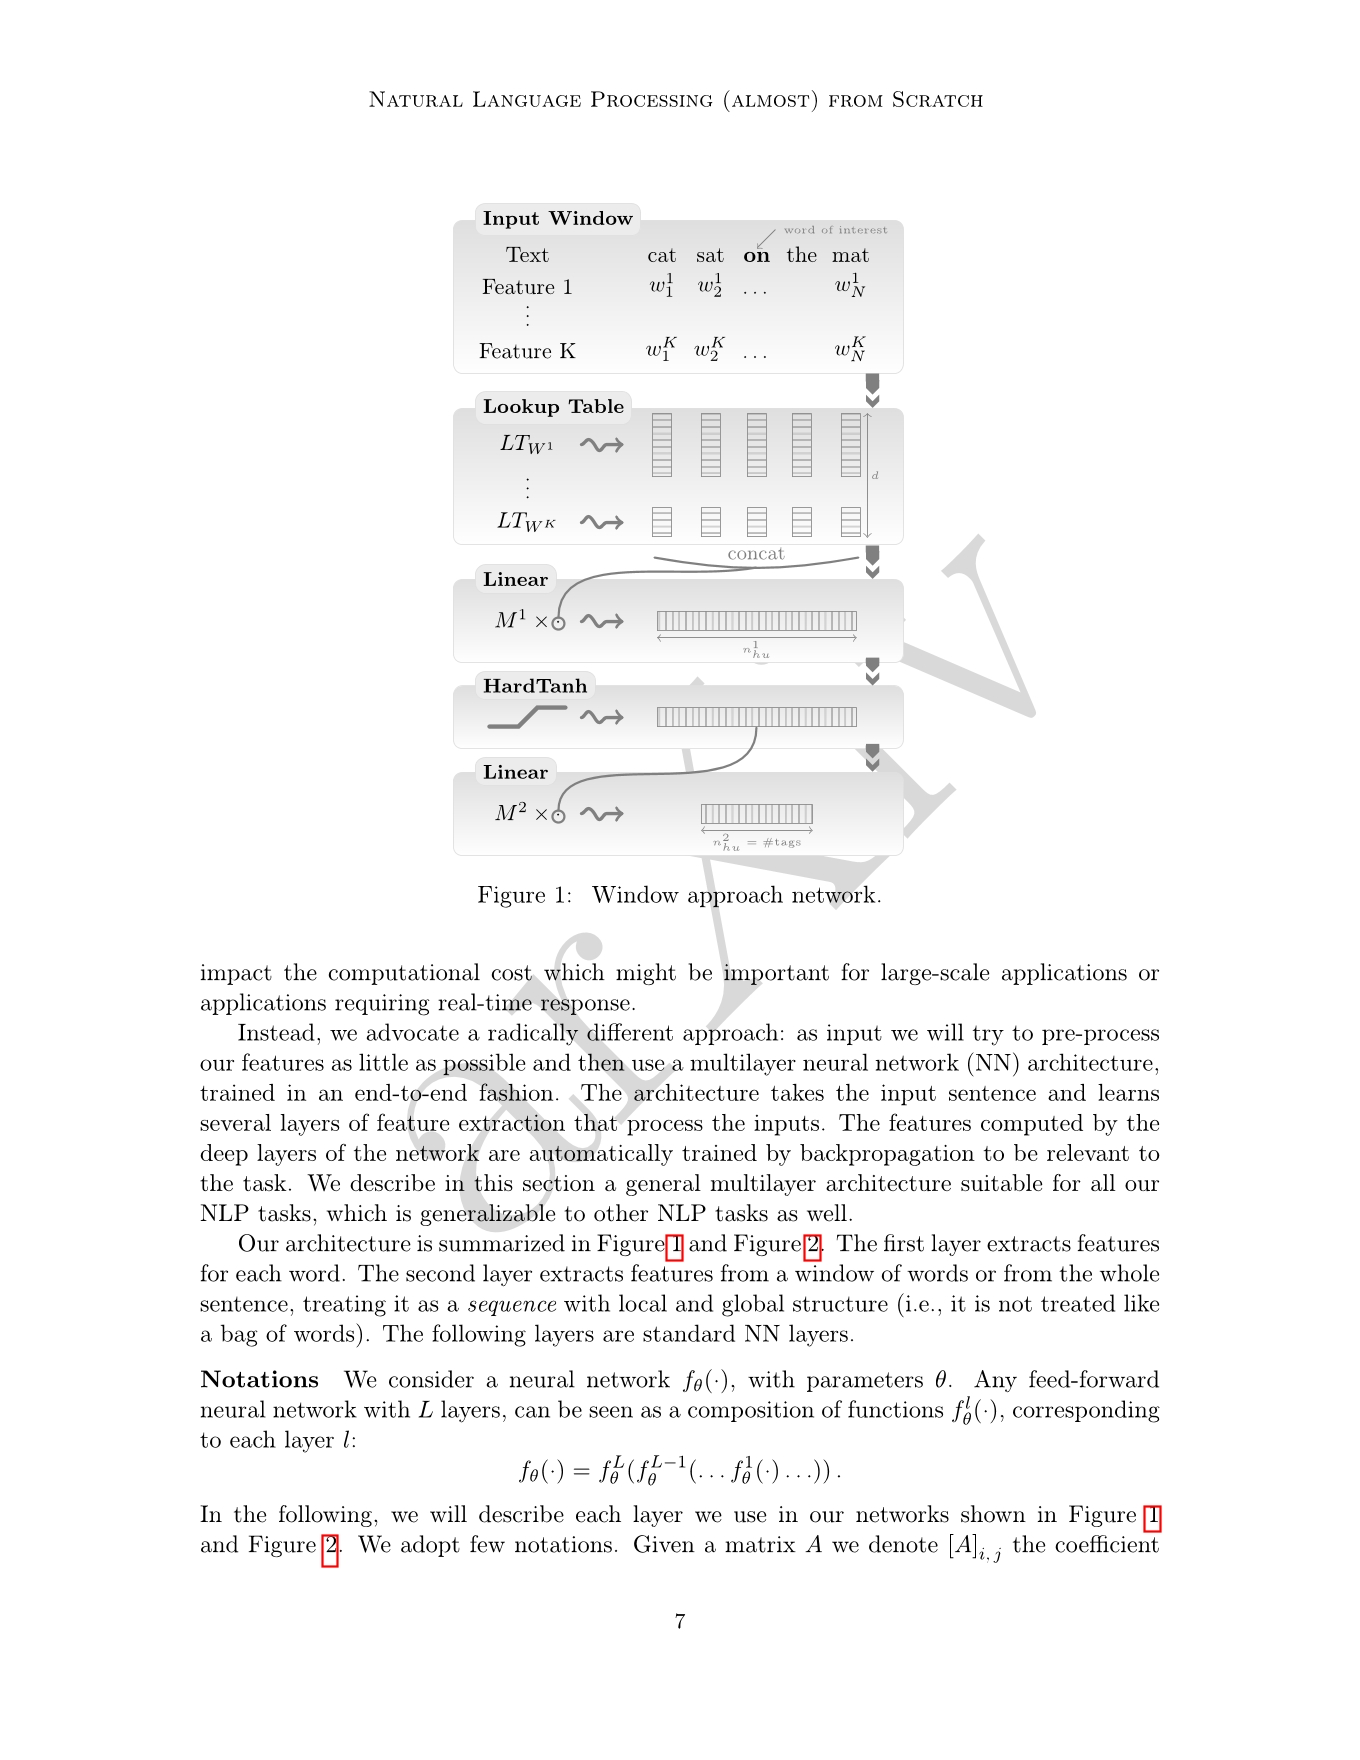
\includegraphics[width=\textwidth]{translations/collobert_2011-7.jpg}
\end{center}
\begin{center}
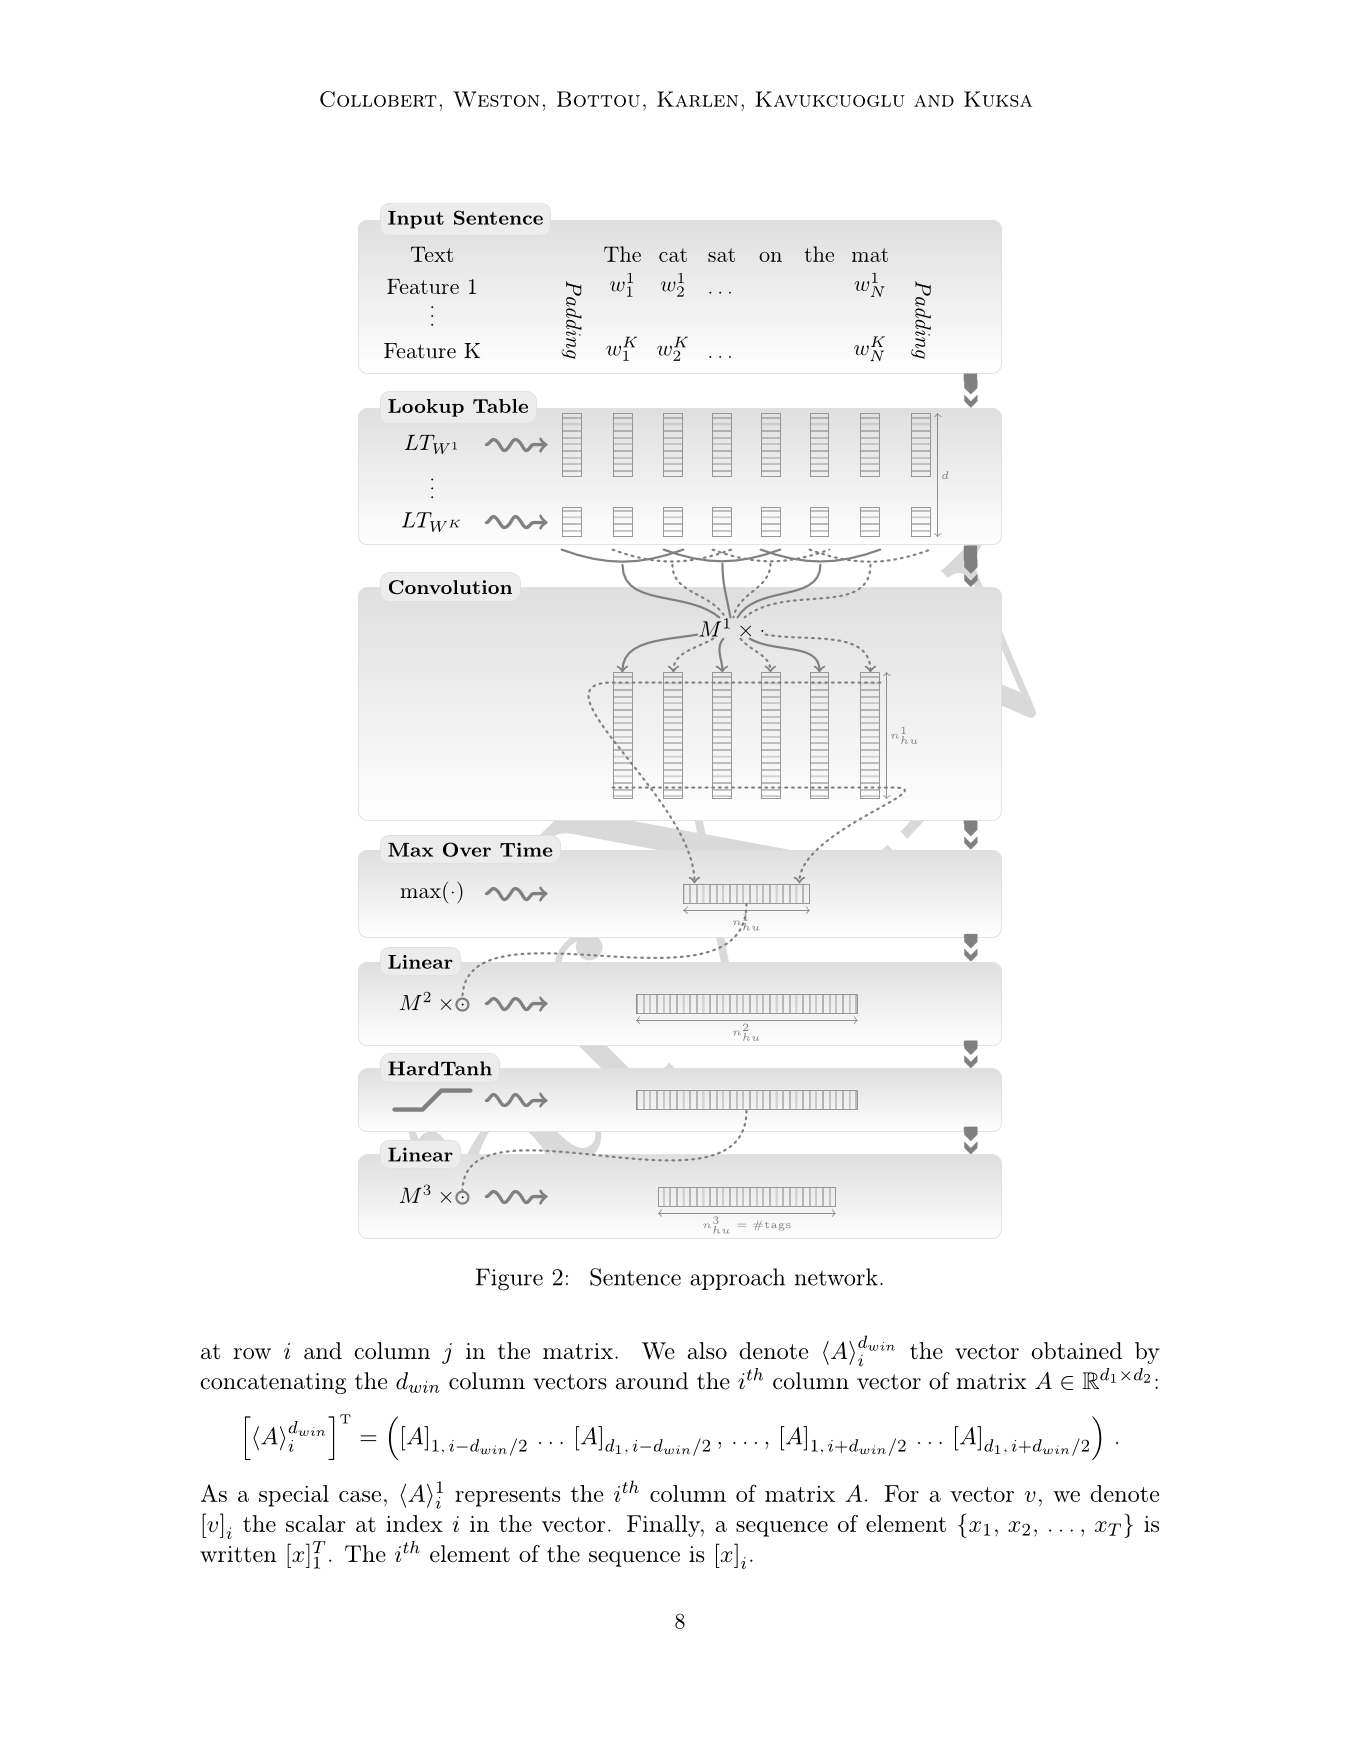
\includegraphics[width=\textwidth]{translations/collobert_2011-8.jpg}
\end{center}
\begin{center}
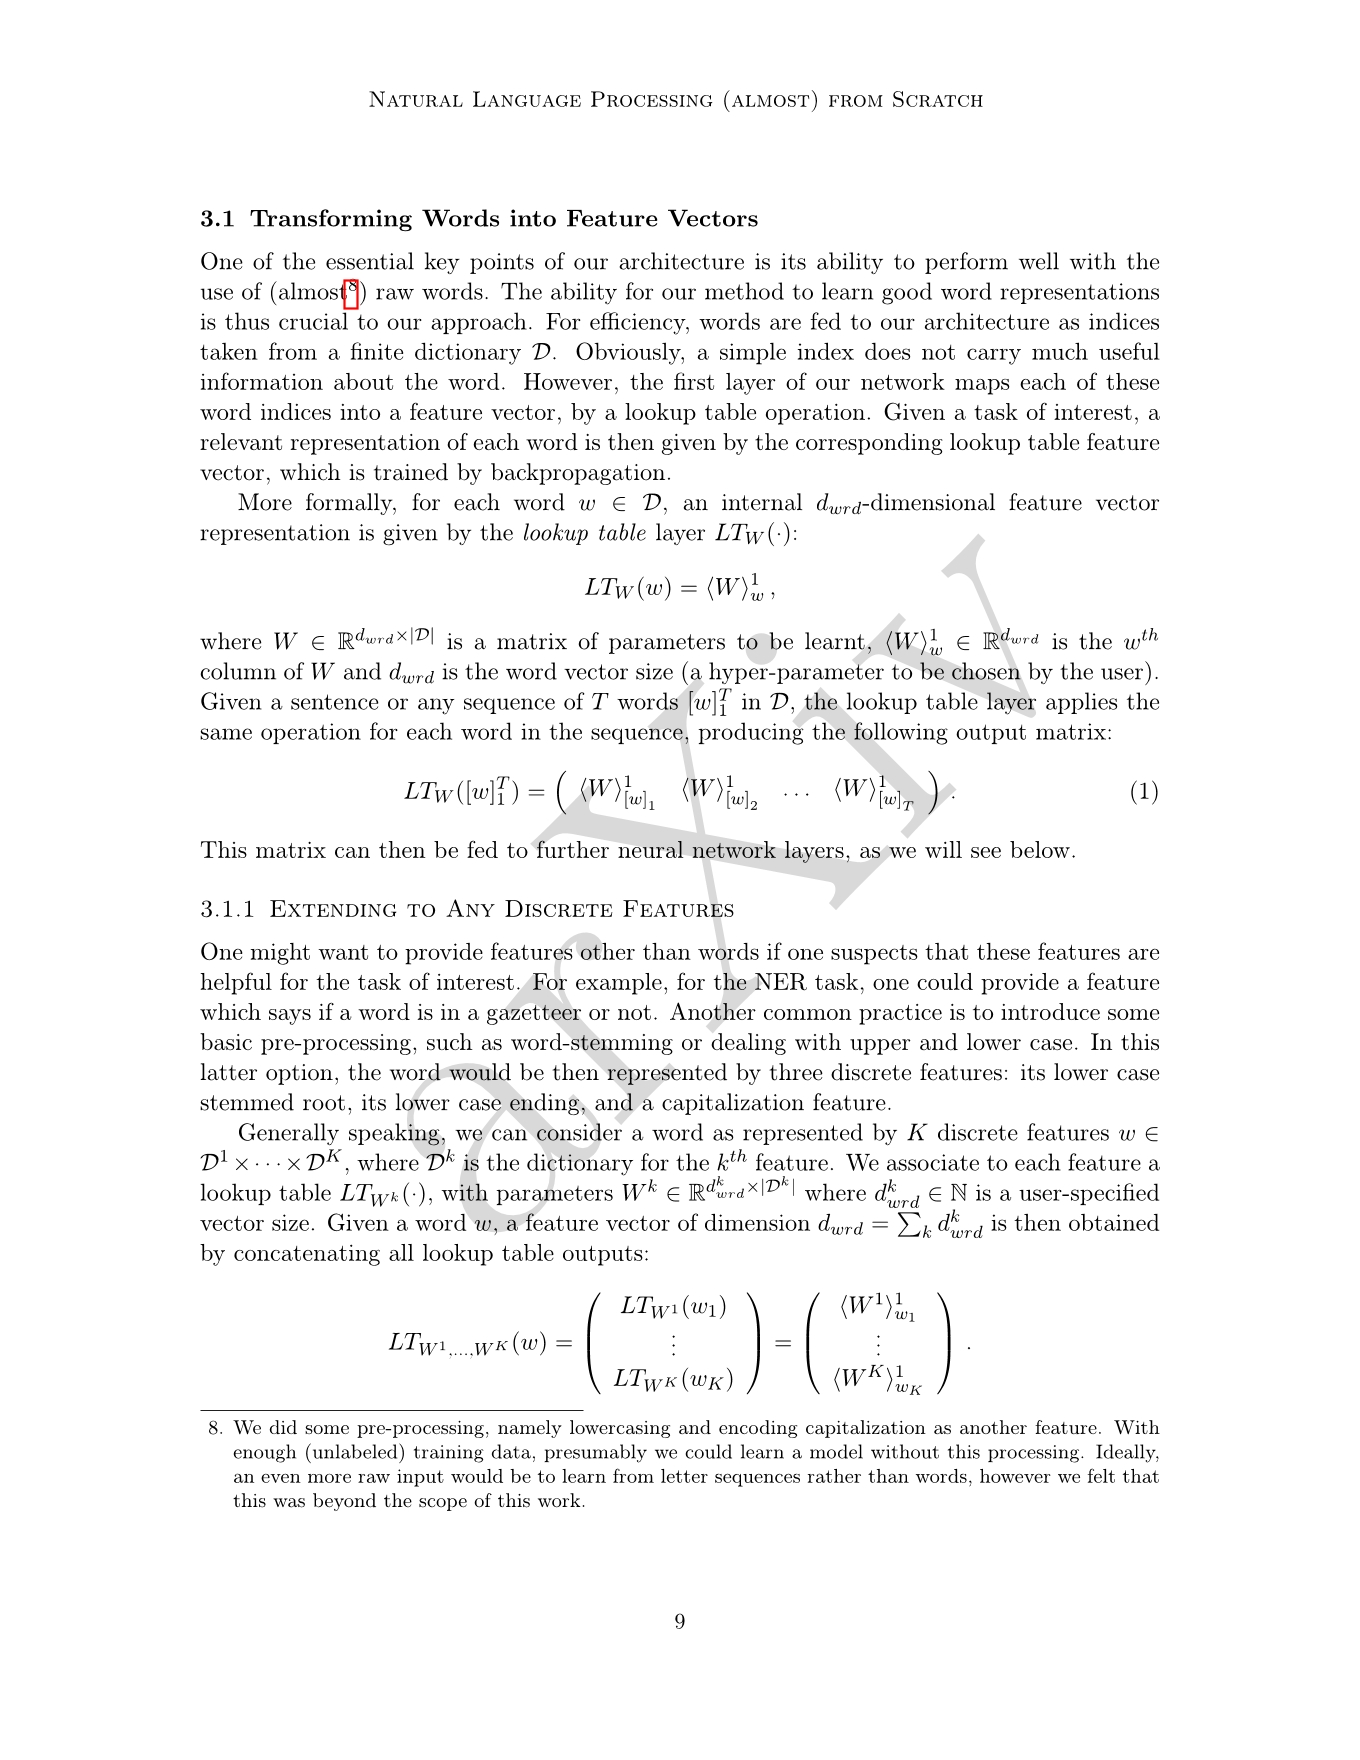
\includegraphics[width=\textwidth]{translations/collobert_2011-9.jpg}
\end{center}
\begin{center}
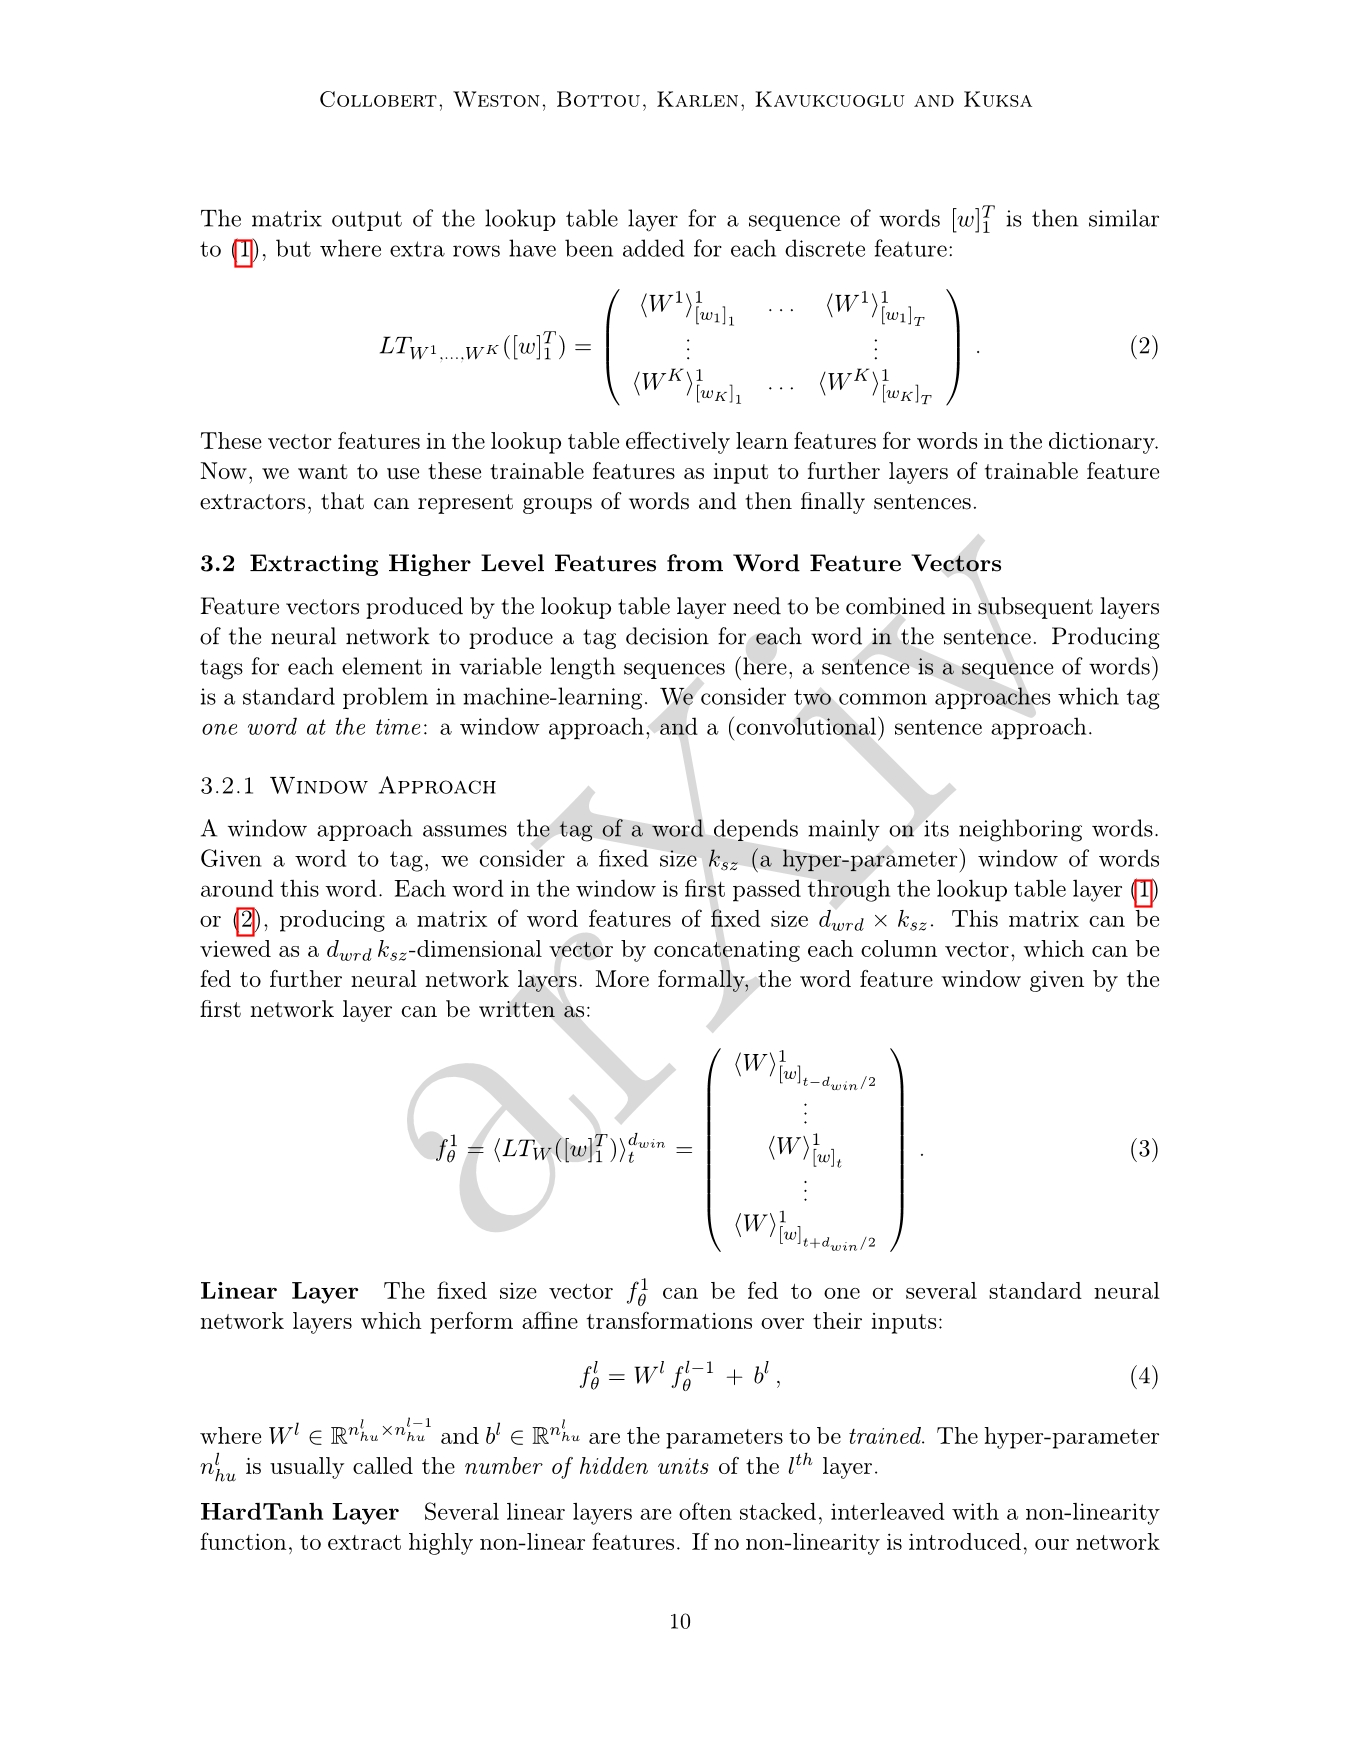
\includegraphics[width=\textwidth]{translations/collobert_2011-10.jpg}
\end{center}
\begin{center}
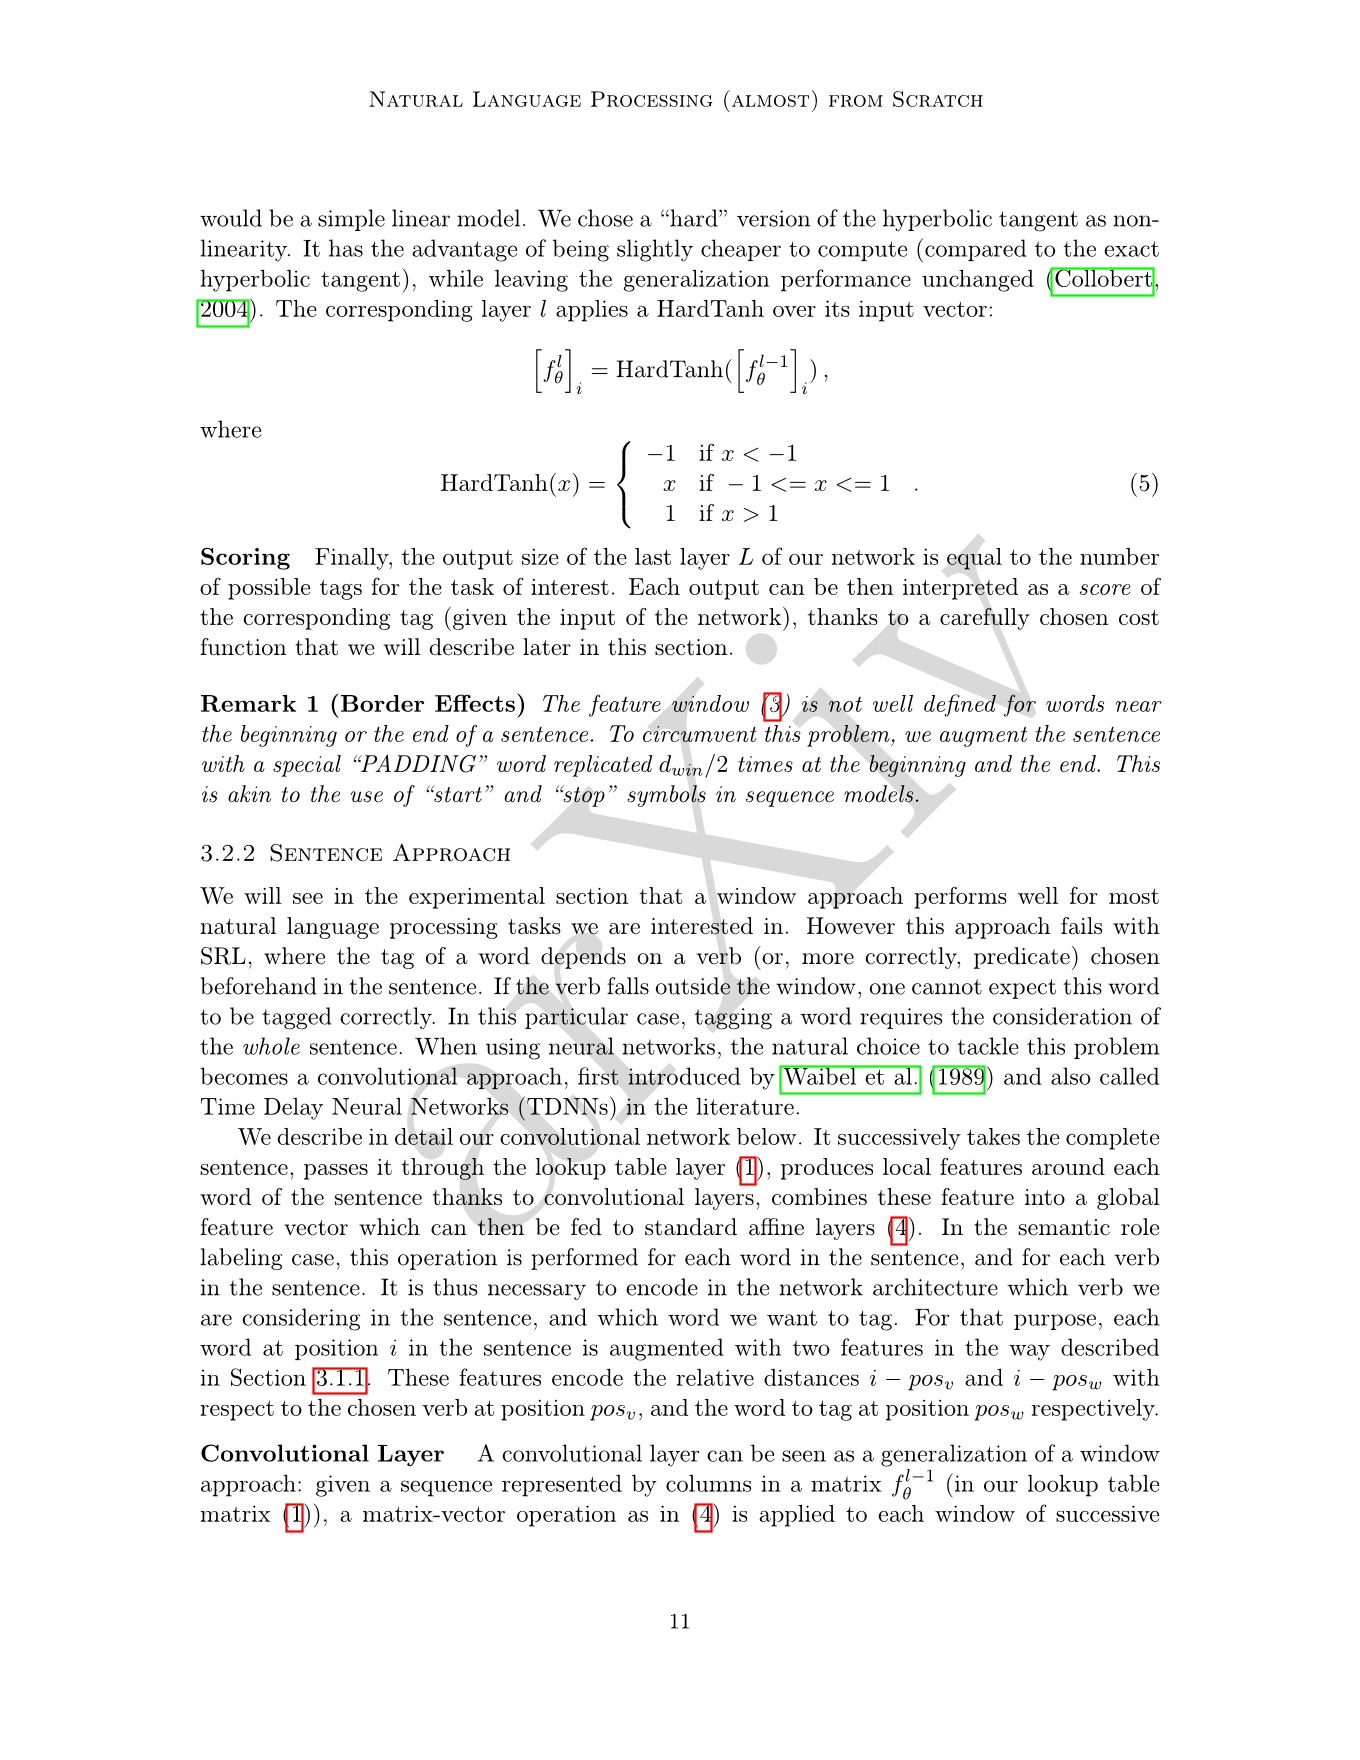
\includegraphics[width=\textwidth]{translations/collobert_2011-11.jpg}
\end{center}
\begin{center}
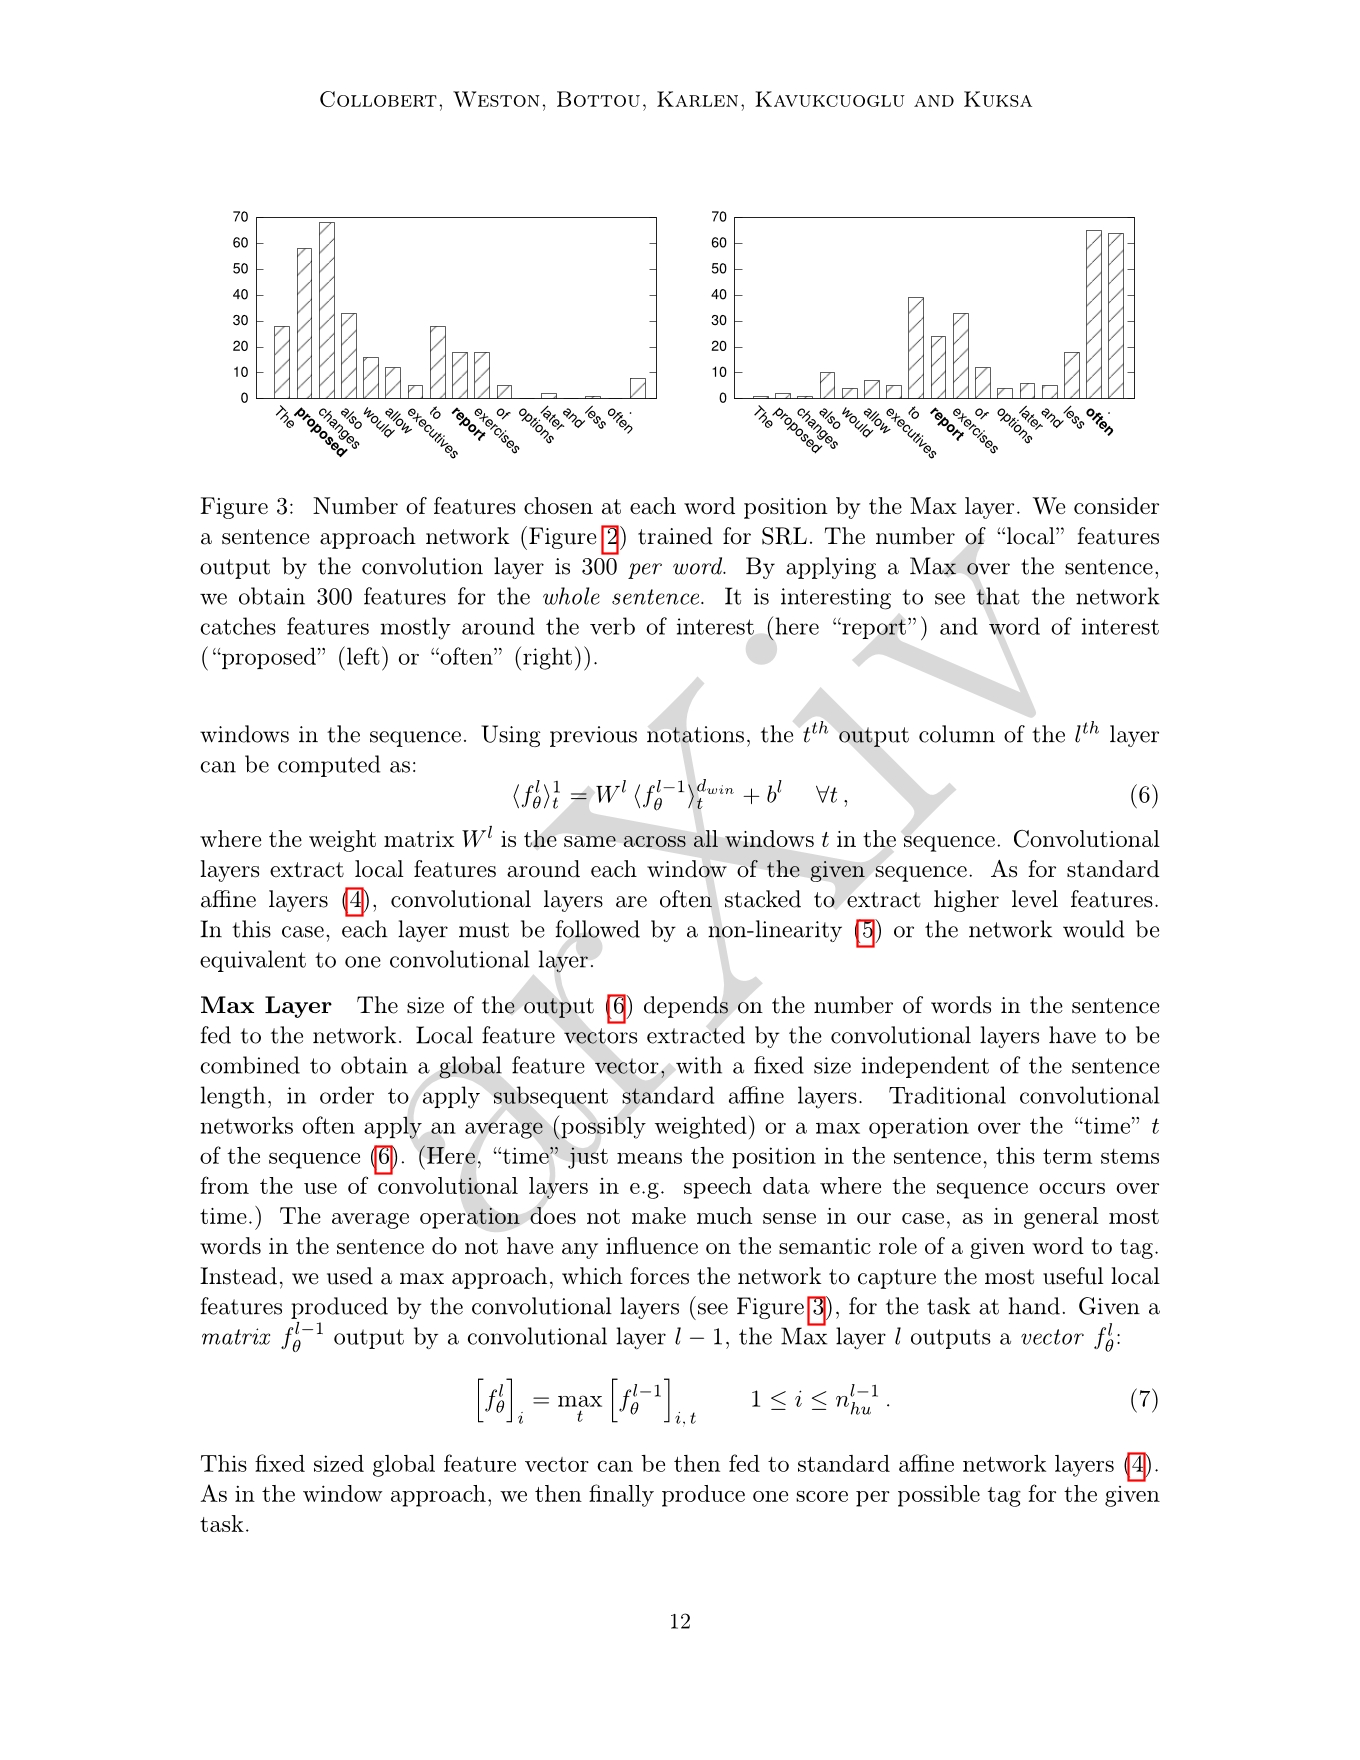
\includegraphics[width=\textwidth]{translations/collobert_2011-12.jpg}
\end{center}
\begin{center}
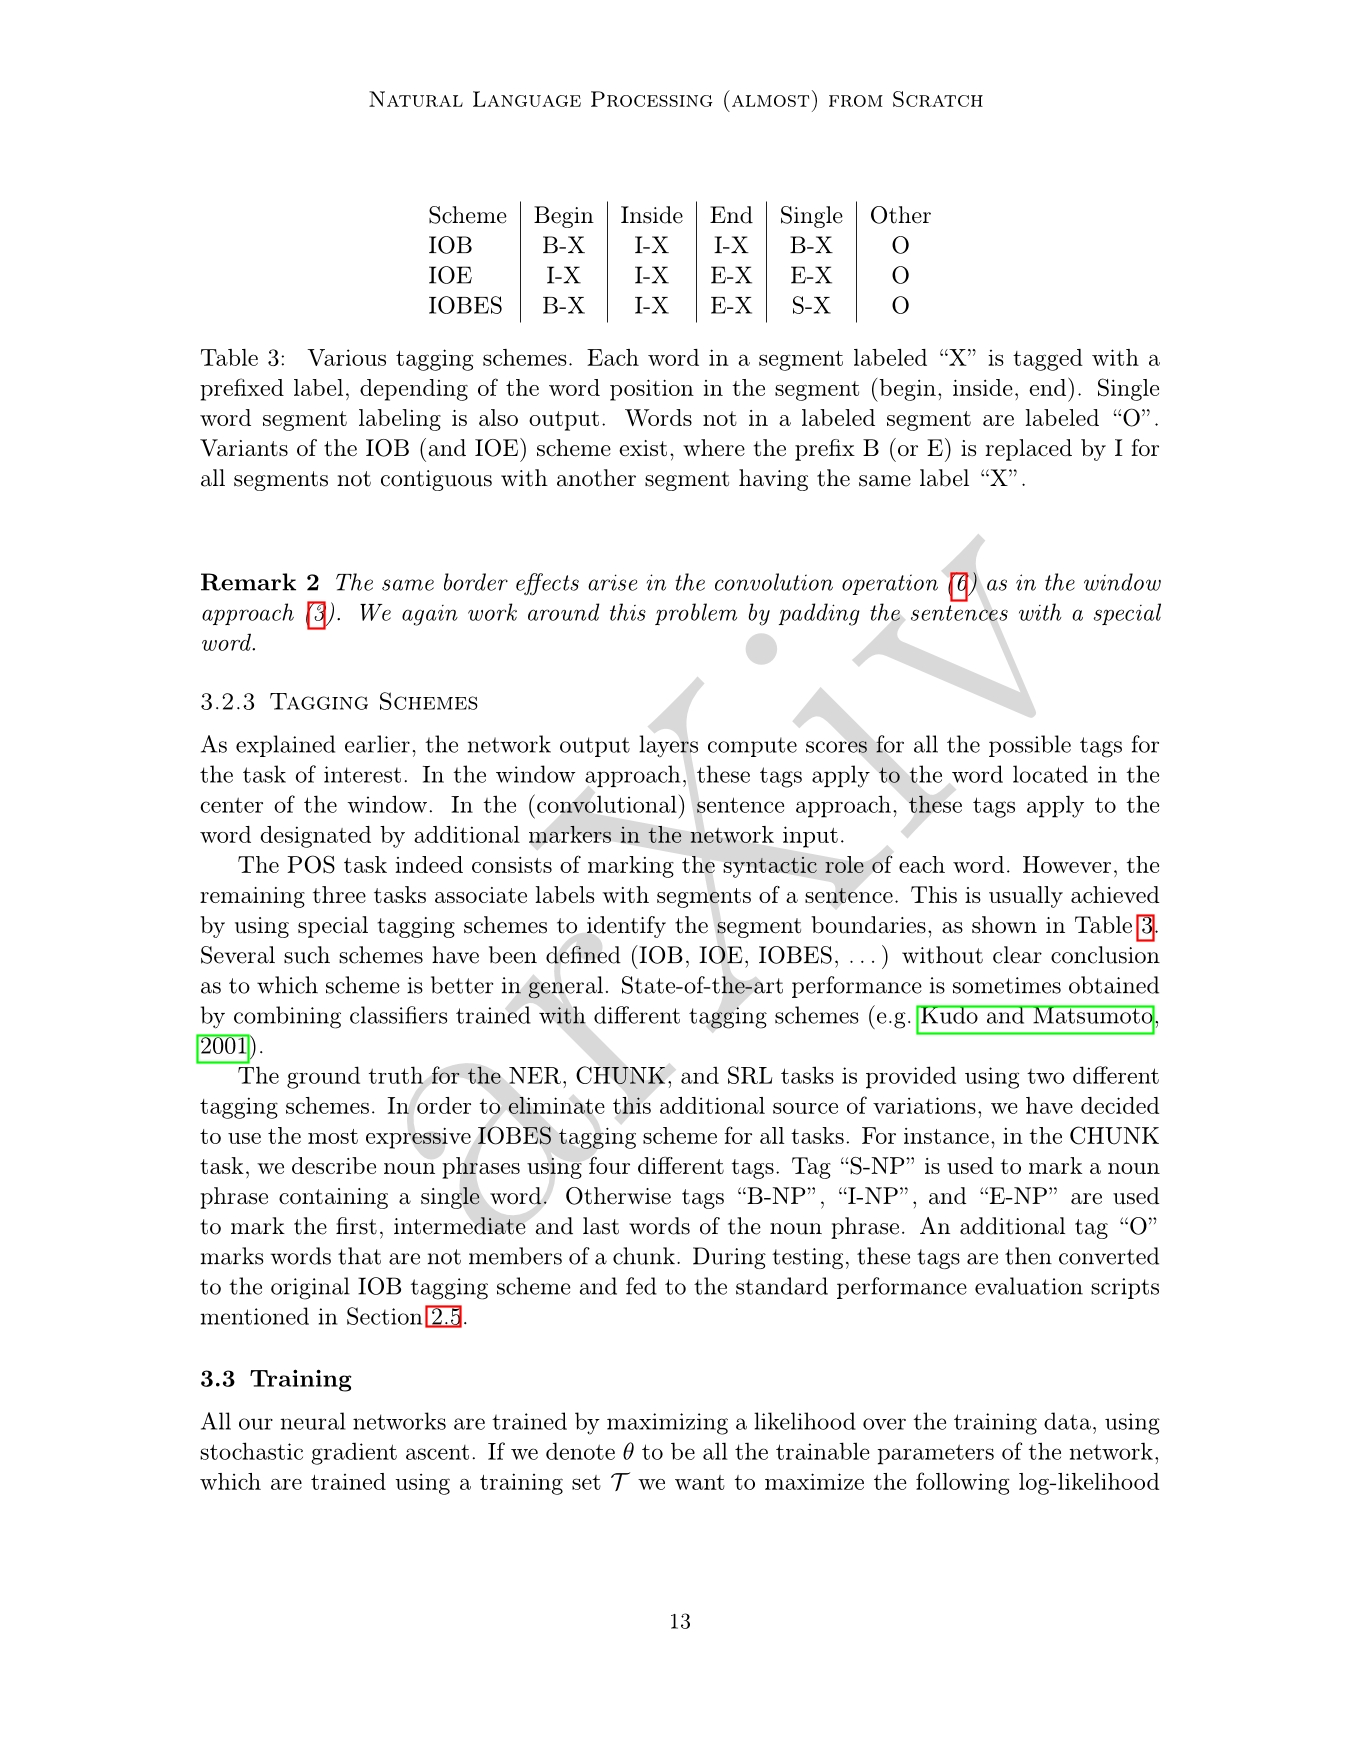
\includegraphics[width=\textwidth]{translations/collobert_2011-13.jpg}
\end{center}
\begin{center}
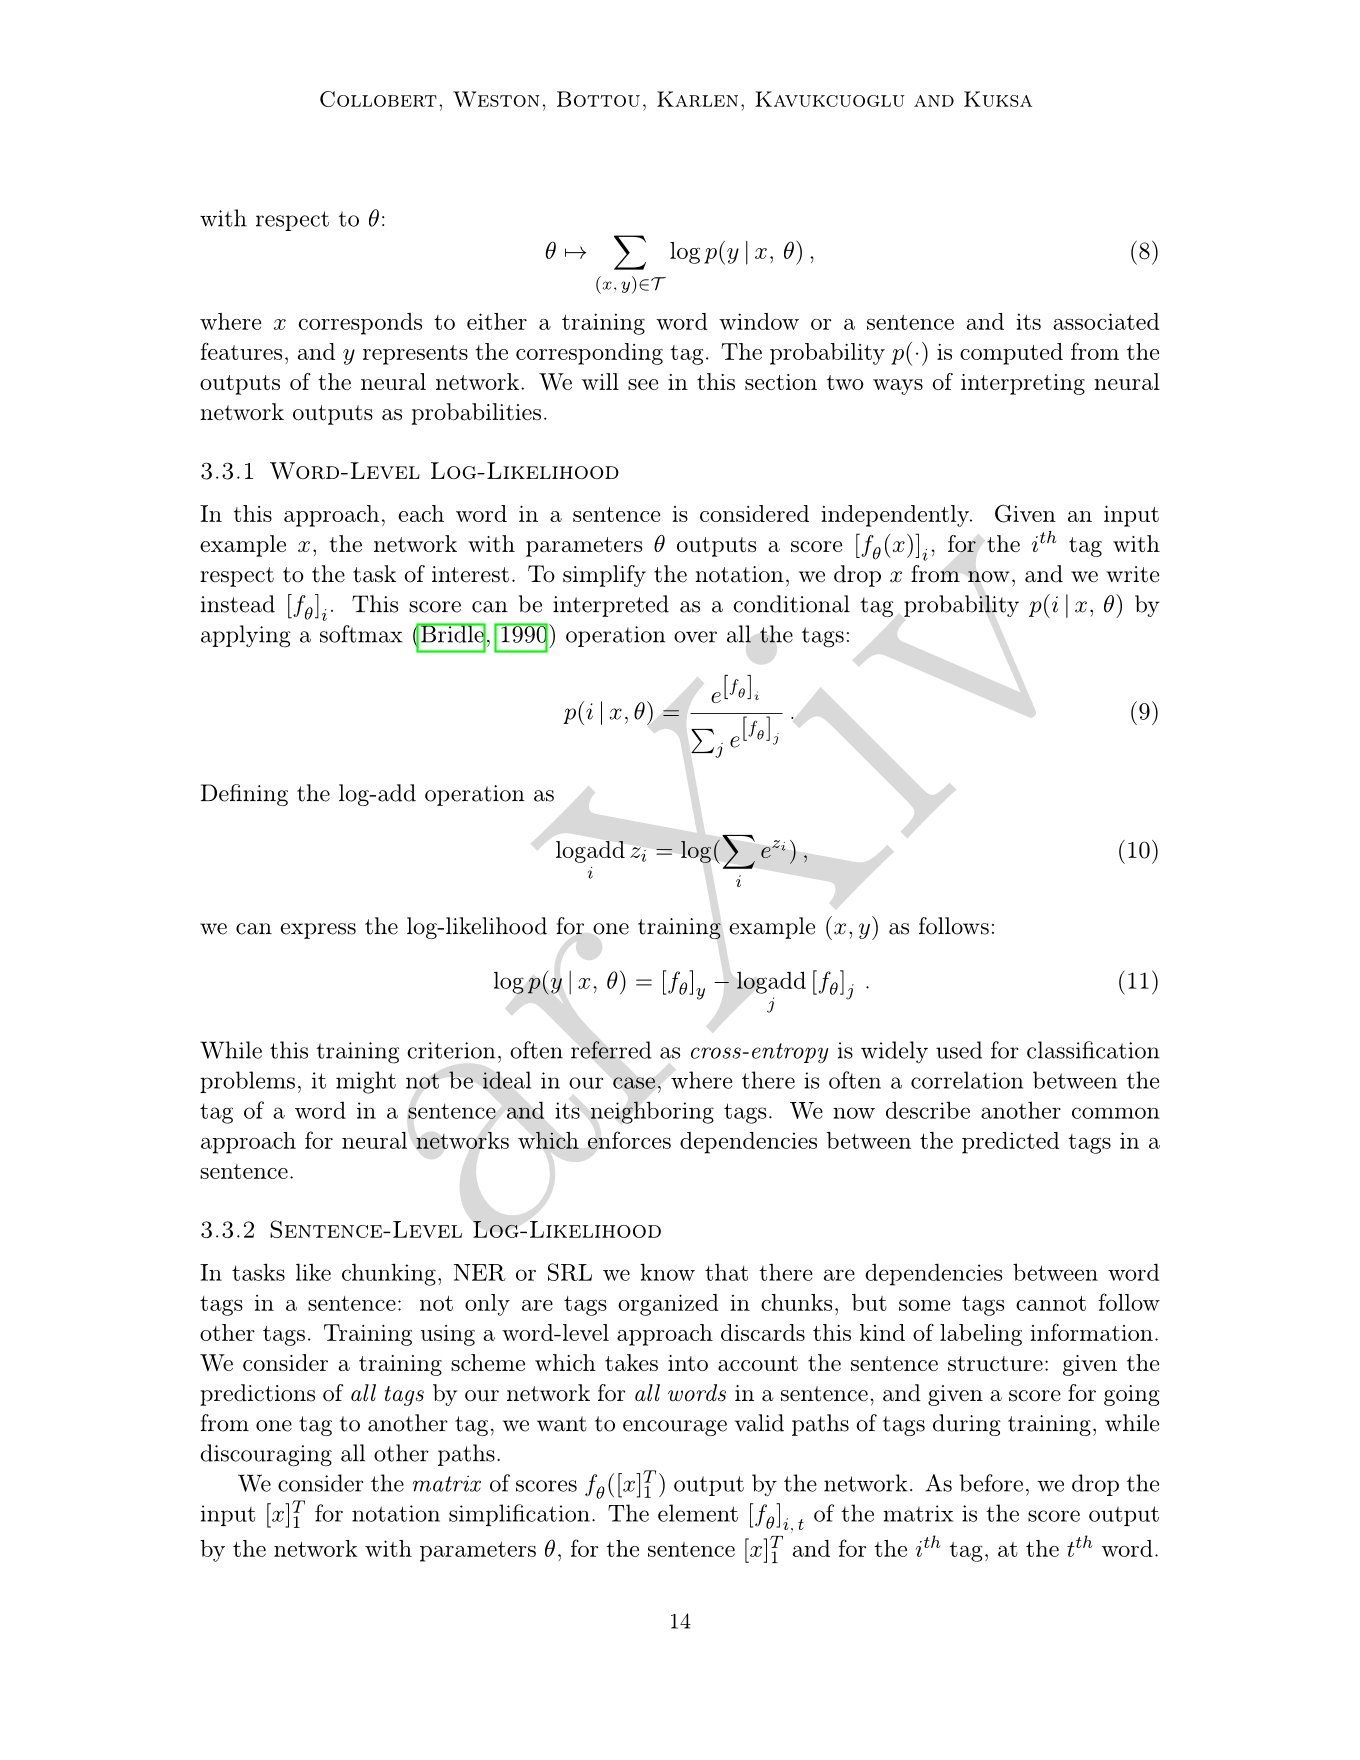
\includegraphics[width=\textwidth]{translations/collobert_2011-14.jpg}
\end{center}
\begin{center}
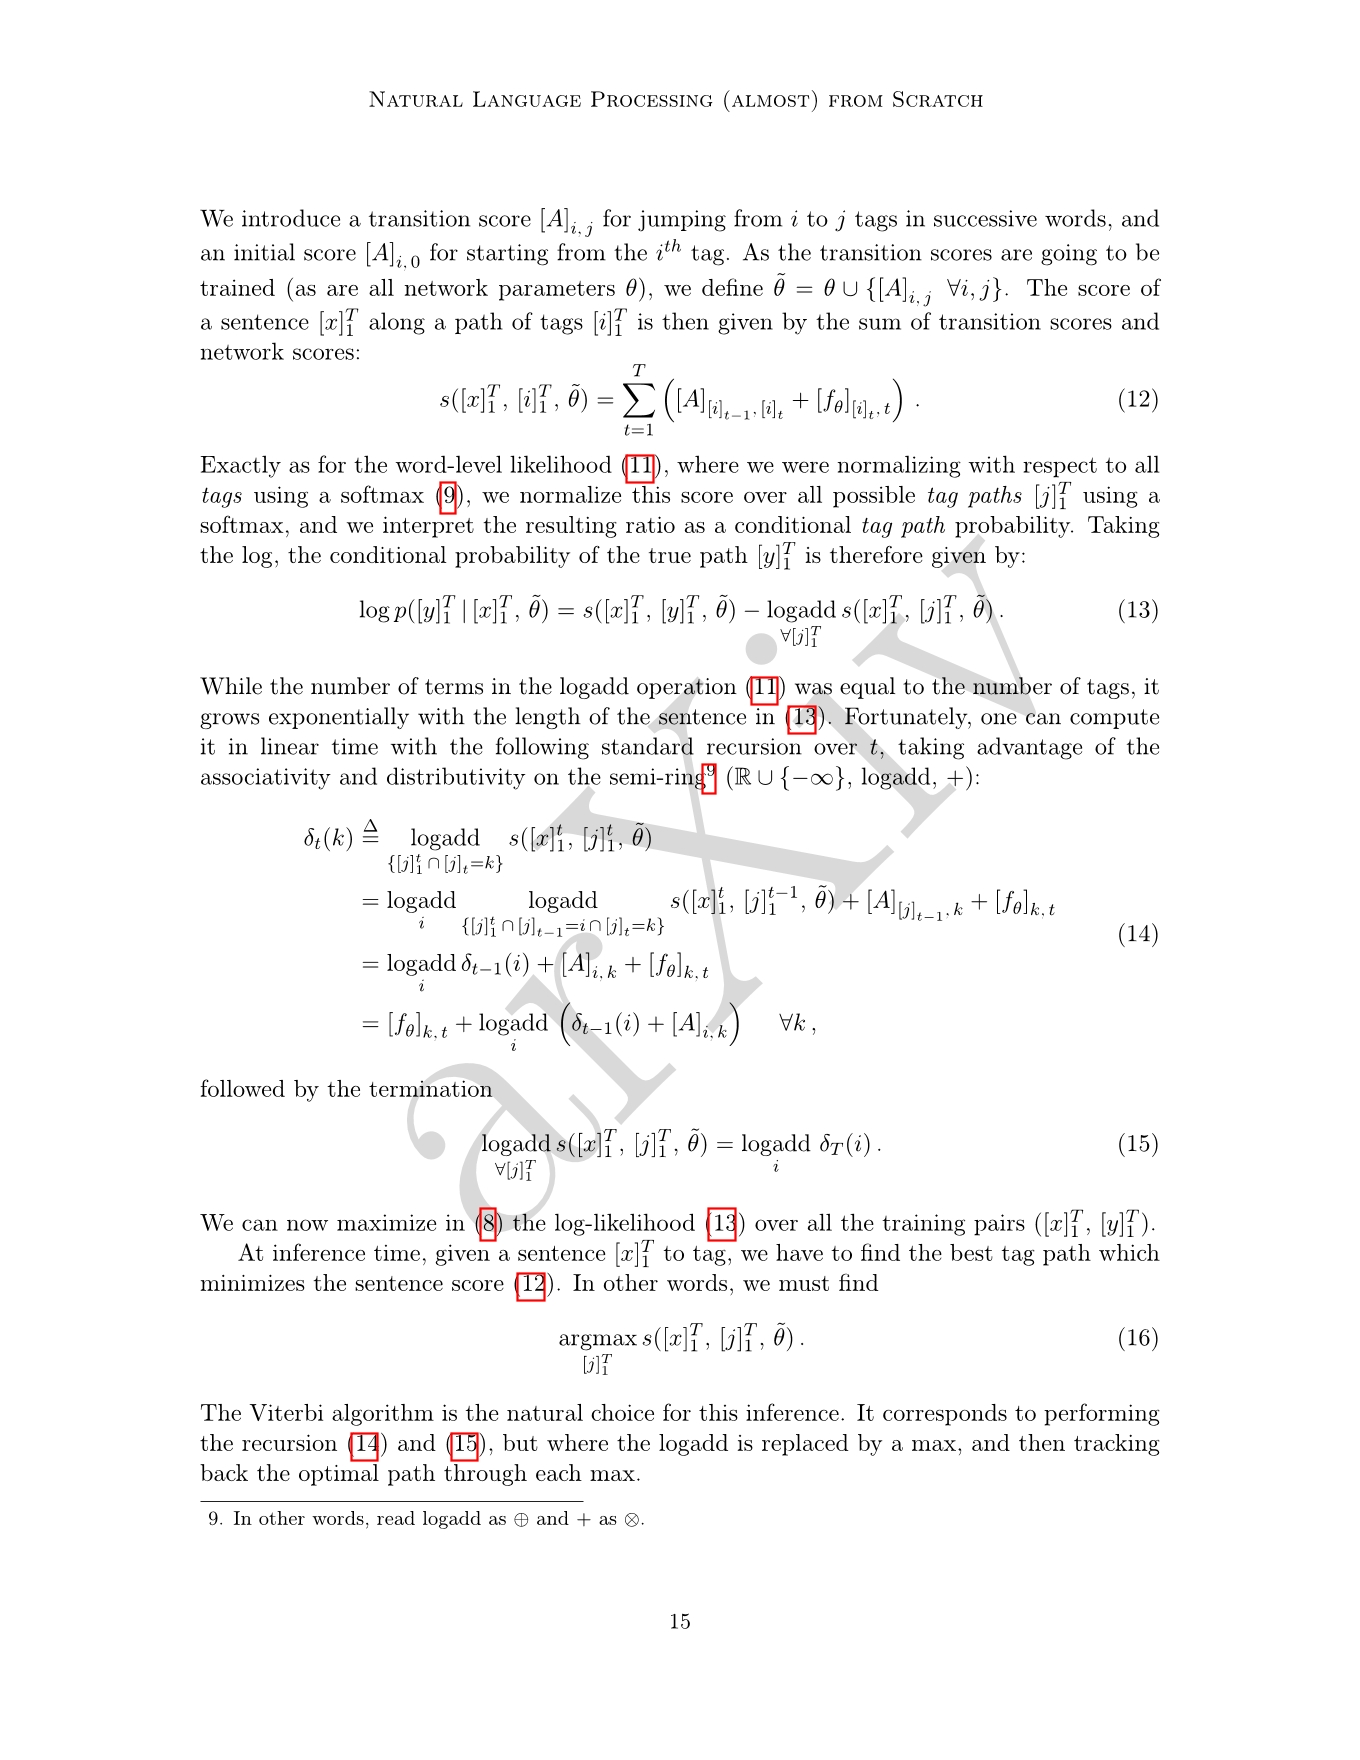
\includegraphics[width=\textwidth]{translations/collobert_2011-15.jpg}
\end{center}
\begin{center}
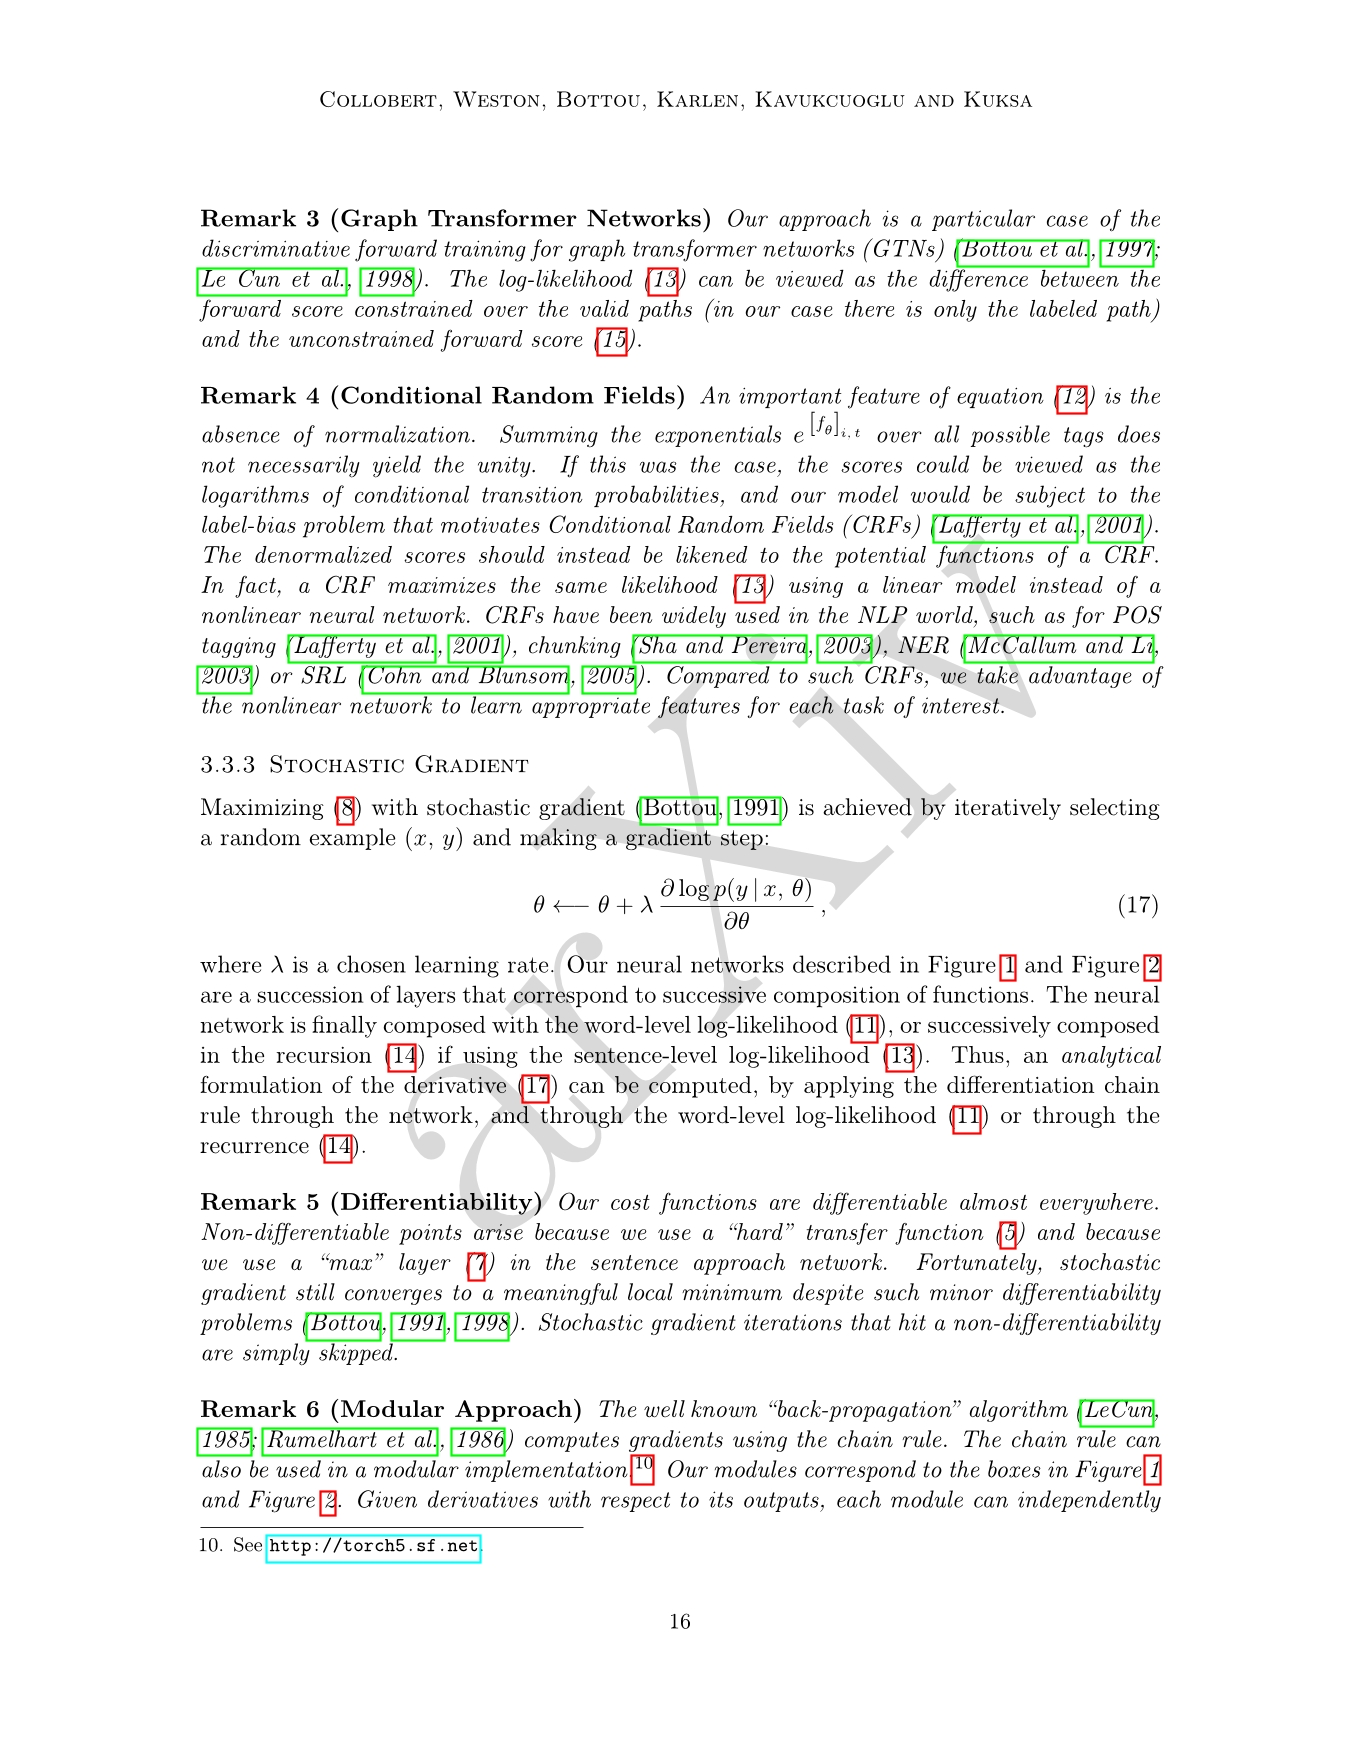
\includegraphics[width=\textwidth]{translations/collobert_2011-16.jpg}
\end{center}
\begin{center}
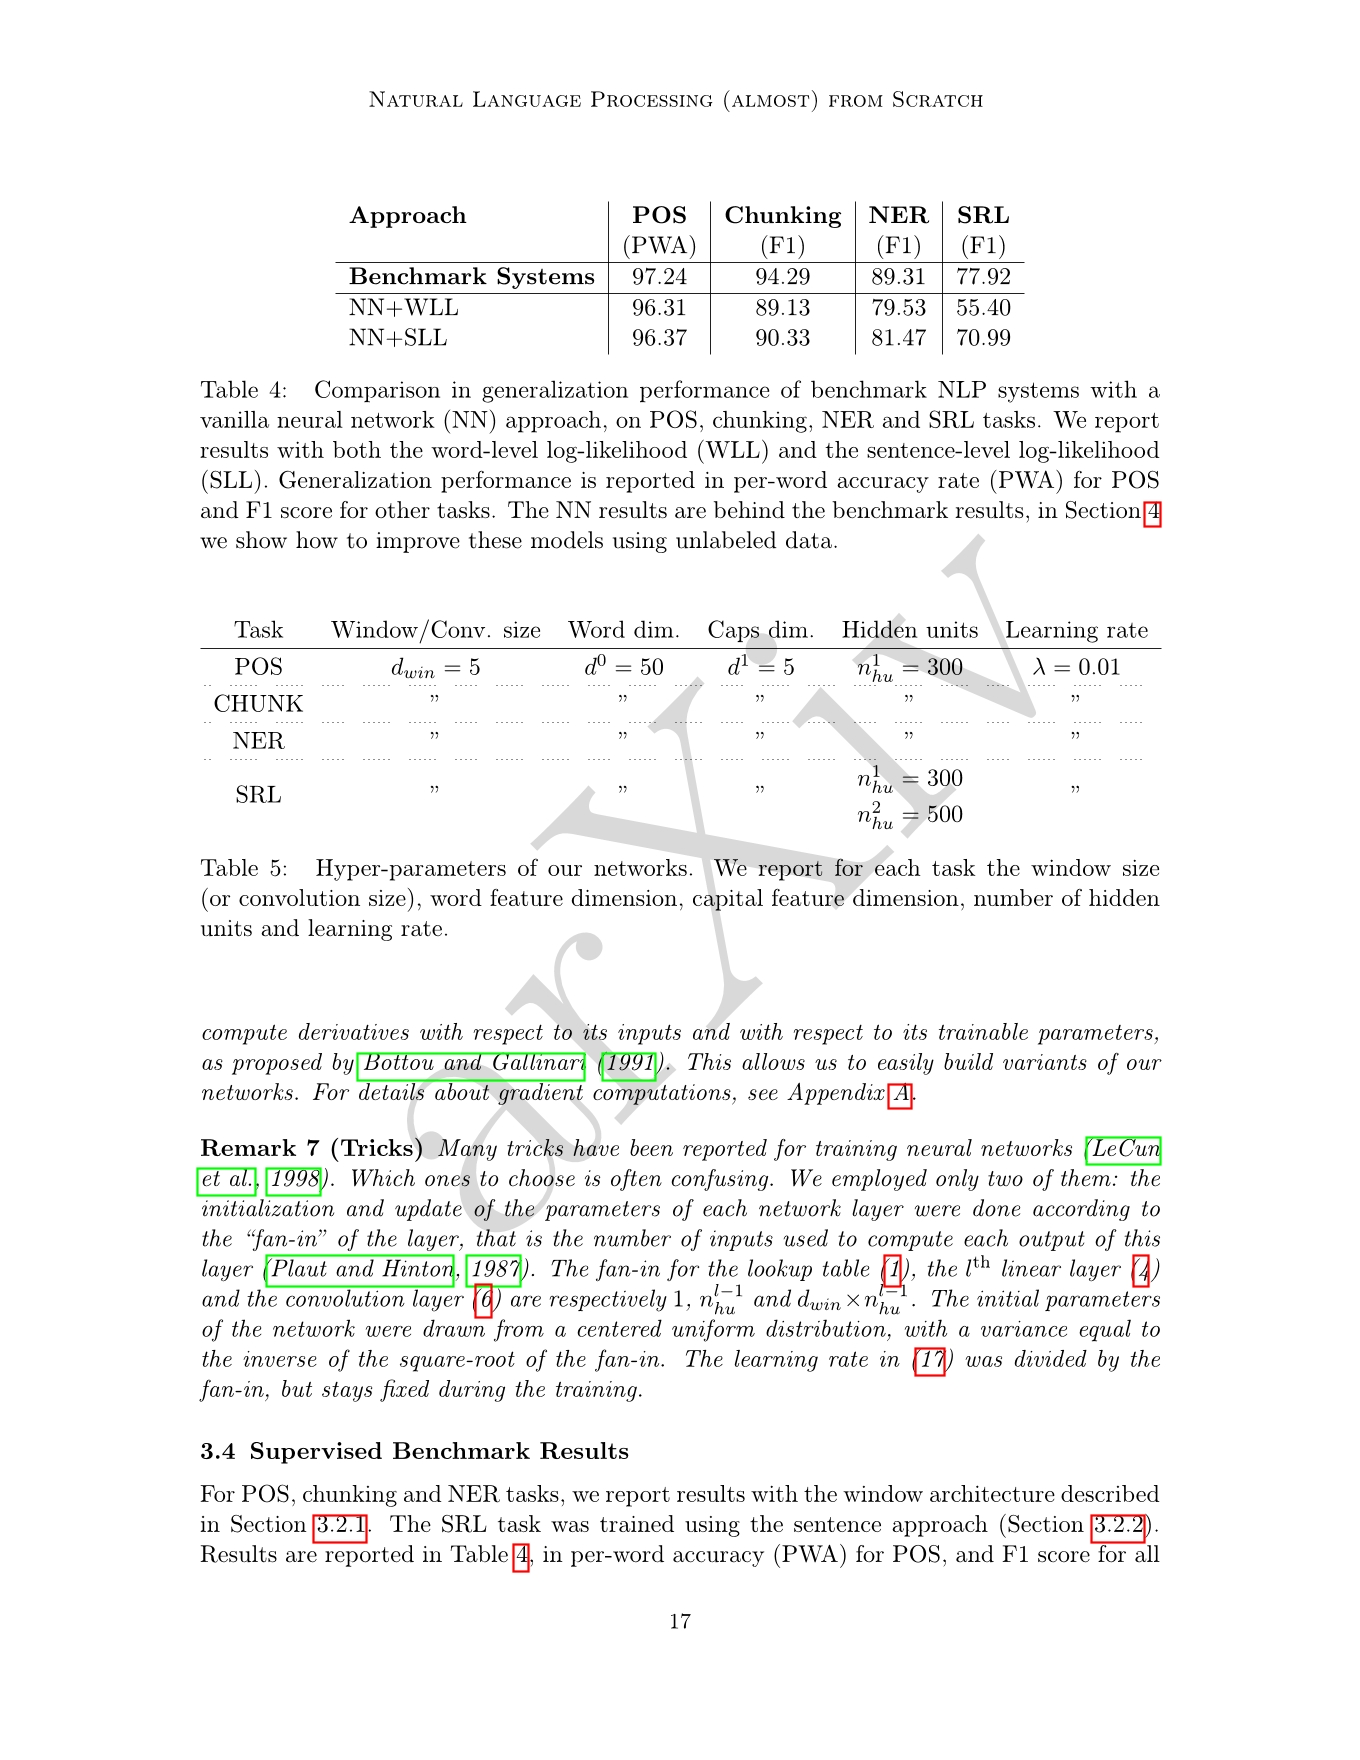
\includegraphics[width=\textwidth]{translations/collobert_2011-17.jpg}
\end{center}
\begin{center}
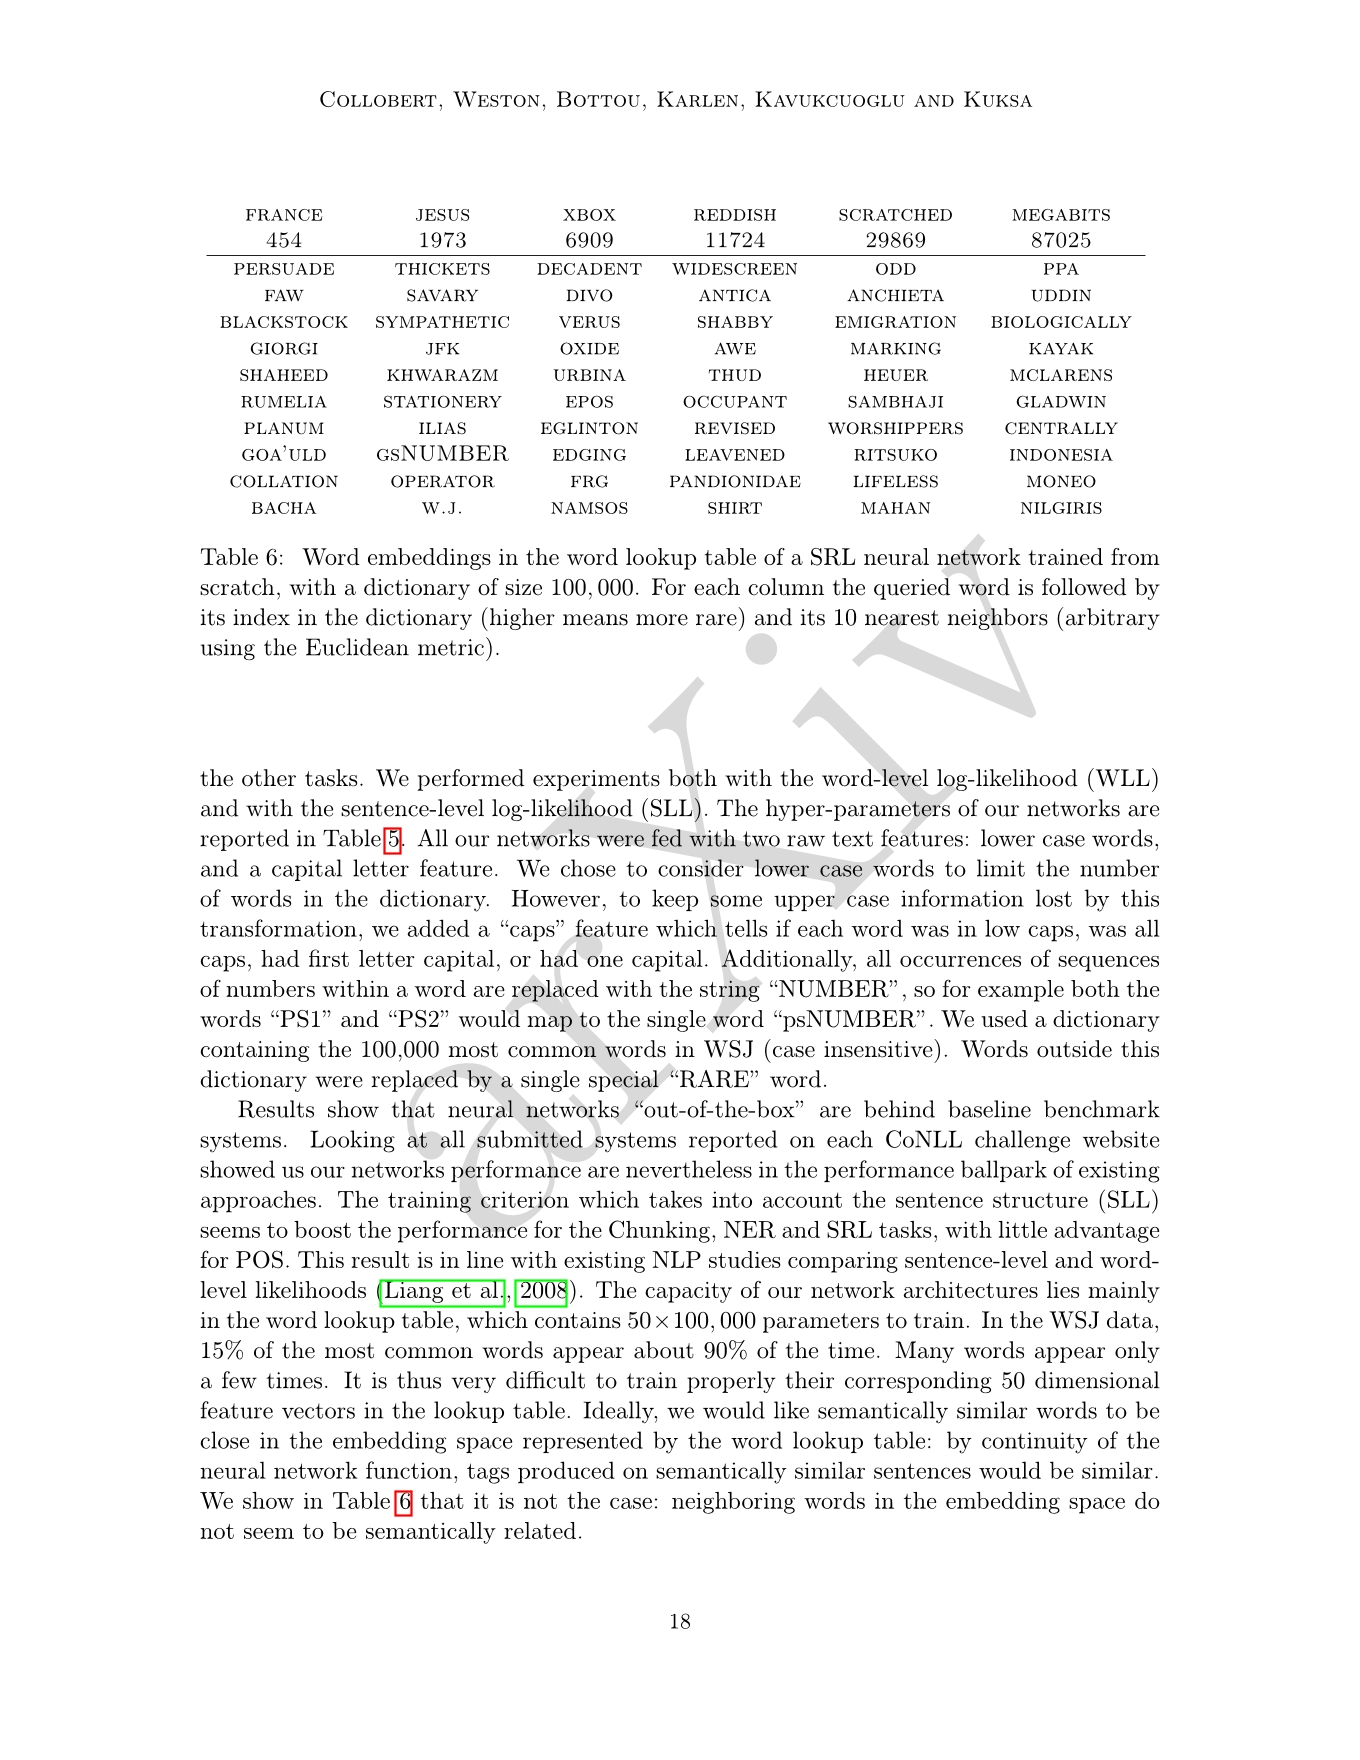
\includegraphics[width=\textwidth]{translations/collobert_2011-18.jpg}
\end{center}
\begin{center}
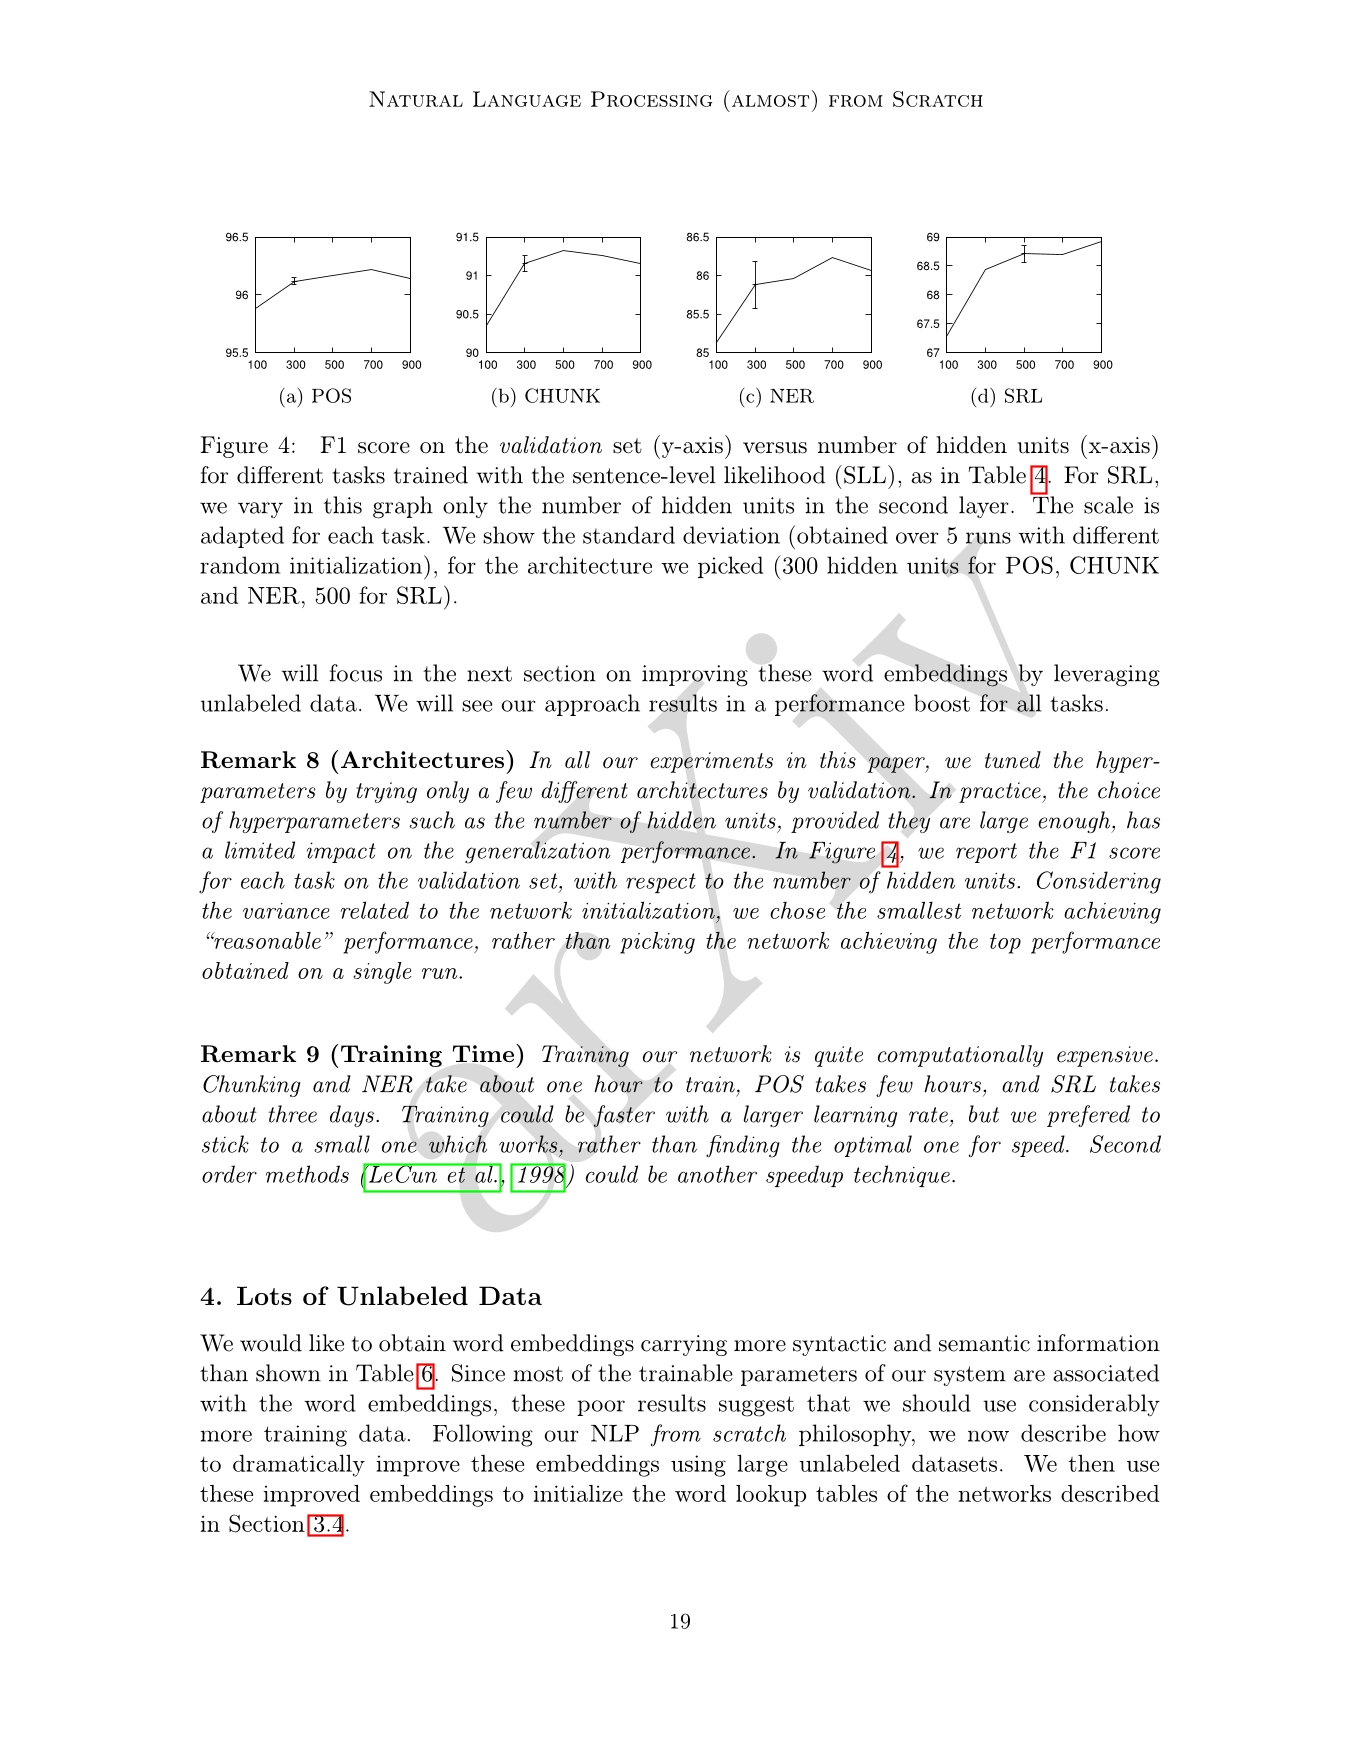
\includegraphics[width=\textwidth]{translations/collobert_2011-19.jpg}
\end{center}
\begin{center}
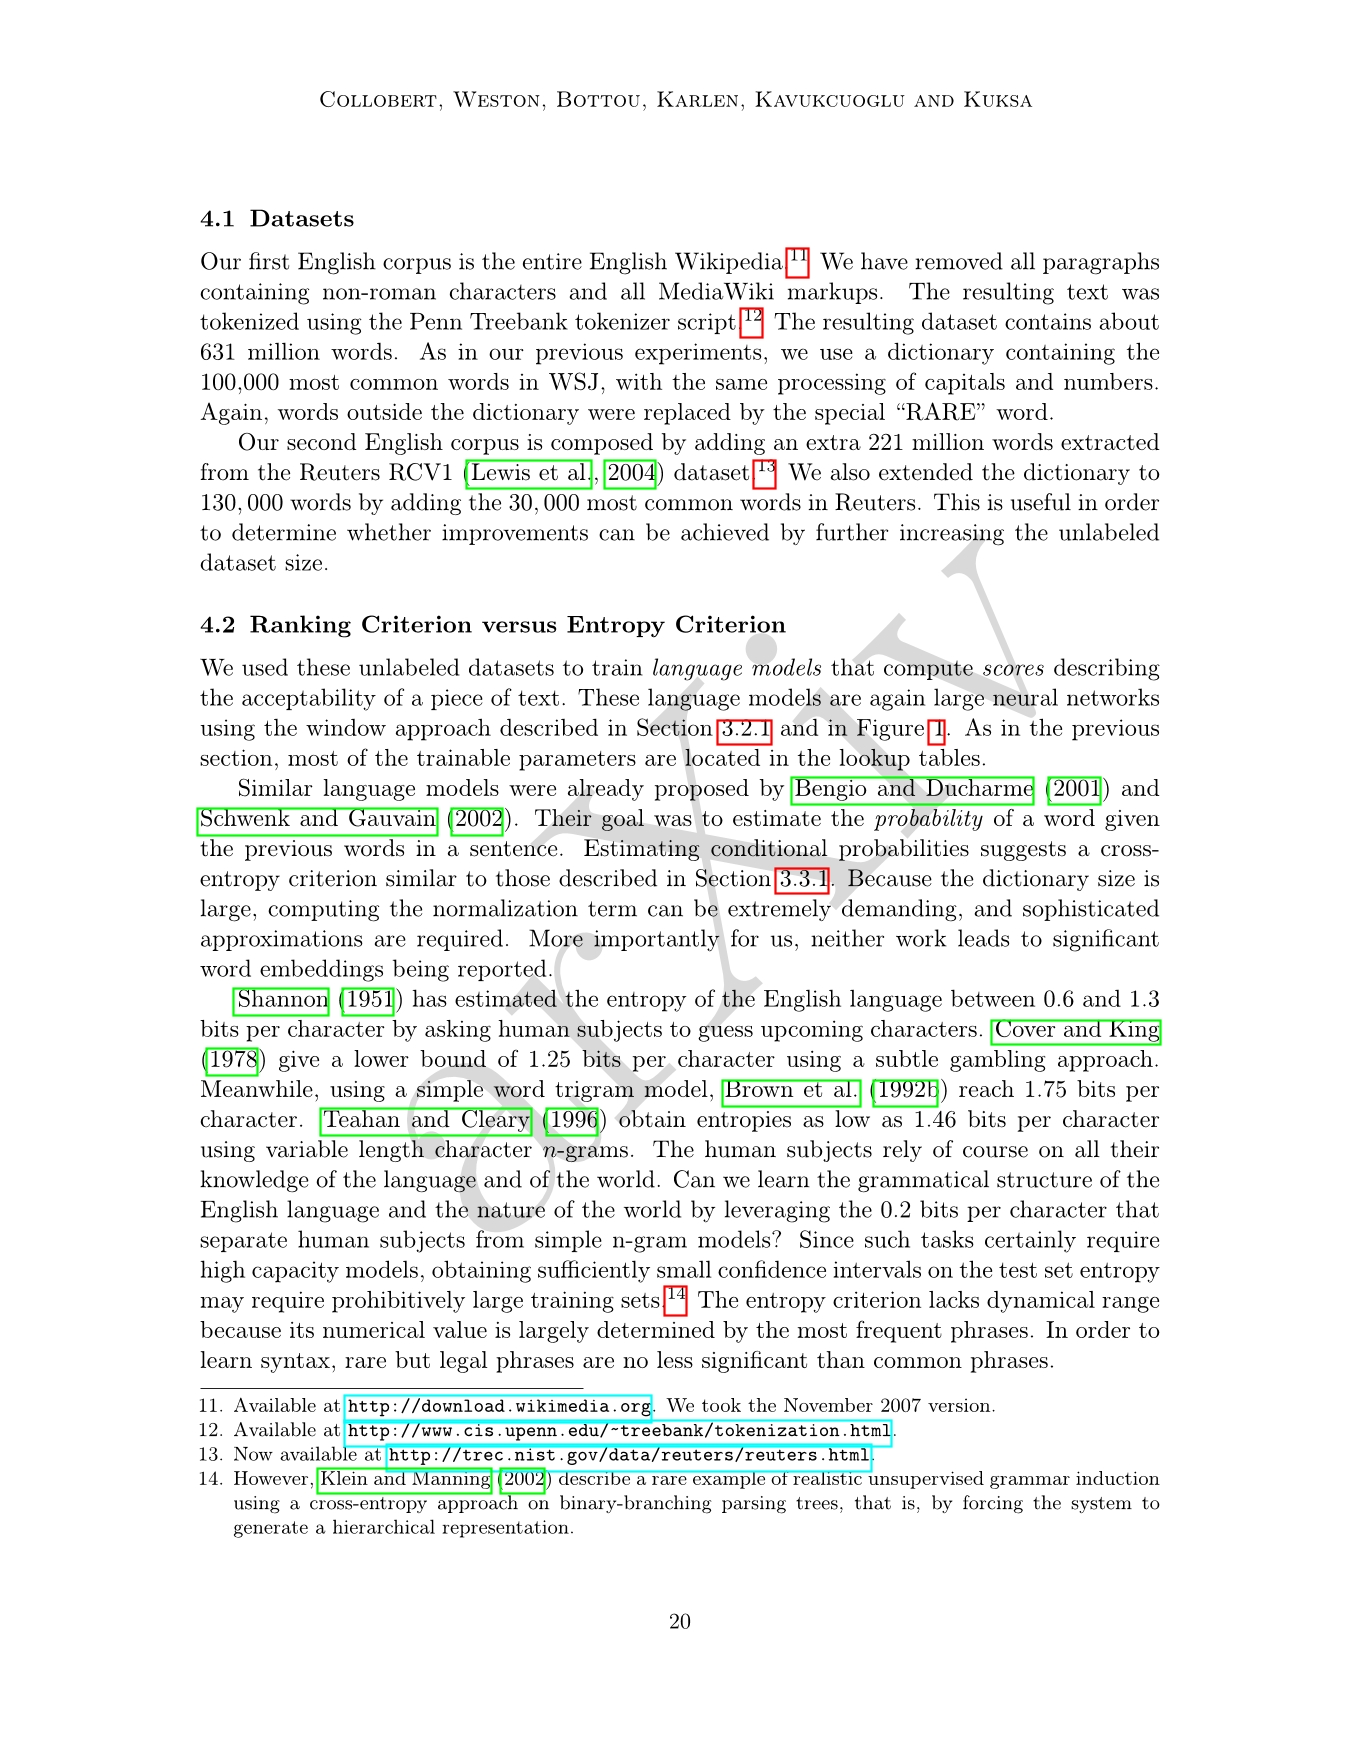
\includegraphics[width=\textwidth]{translations/collobert_2011-20.jpg}
\end{center}
\begin{center}
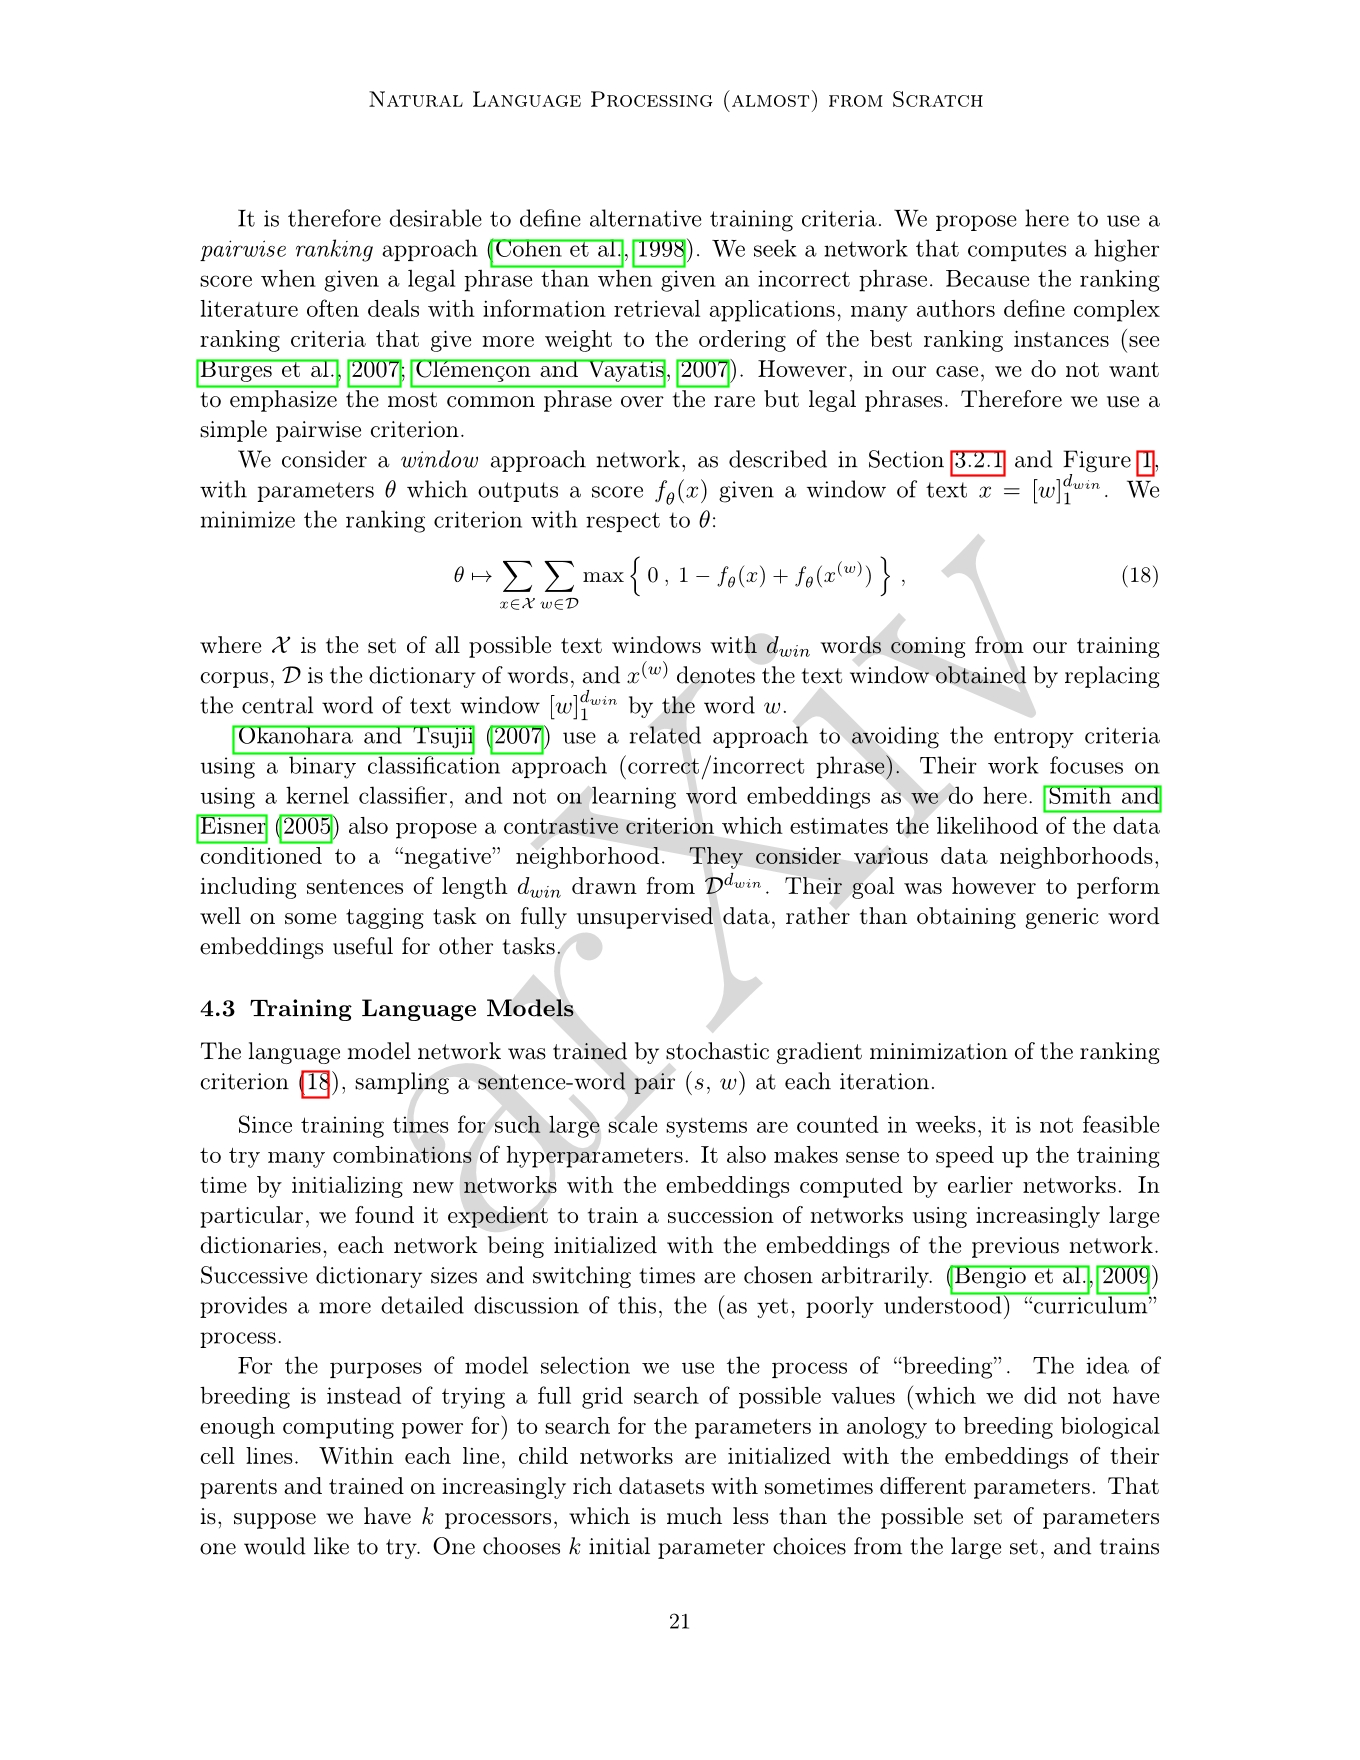
\includegraphics[width=\textwidth]{translations/collobert_2011-21.jpg}
\end{center}
\begin{center}
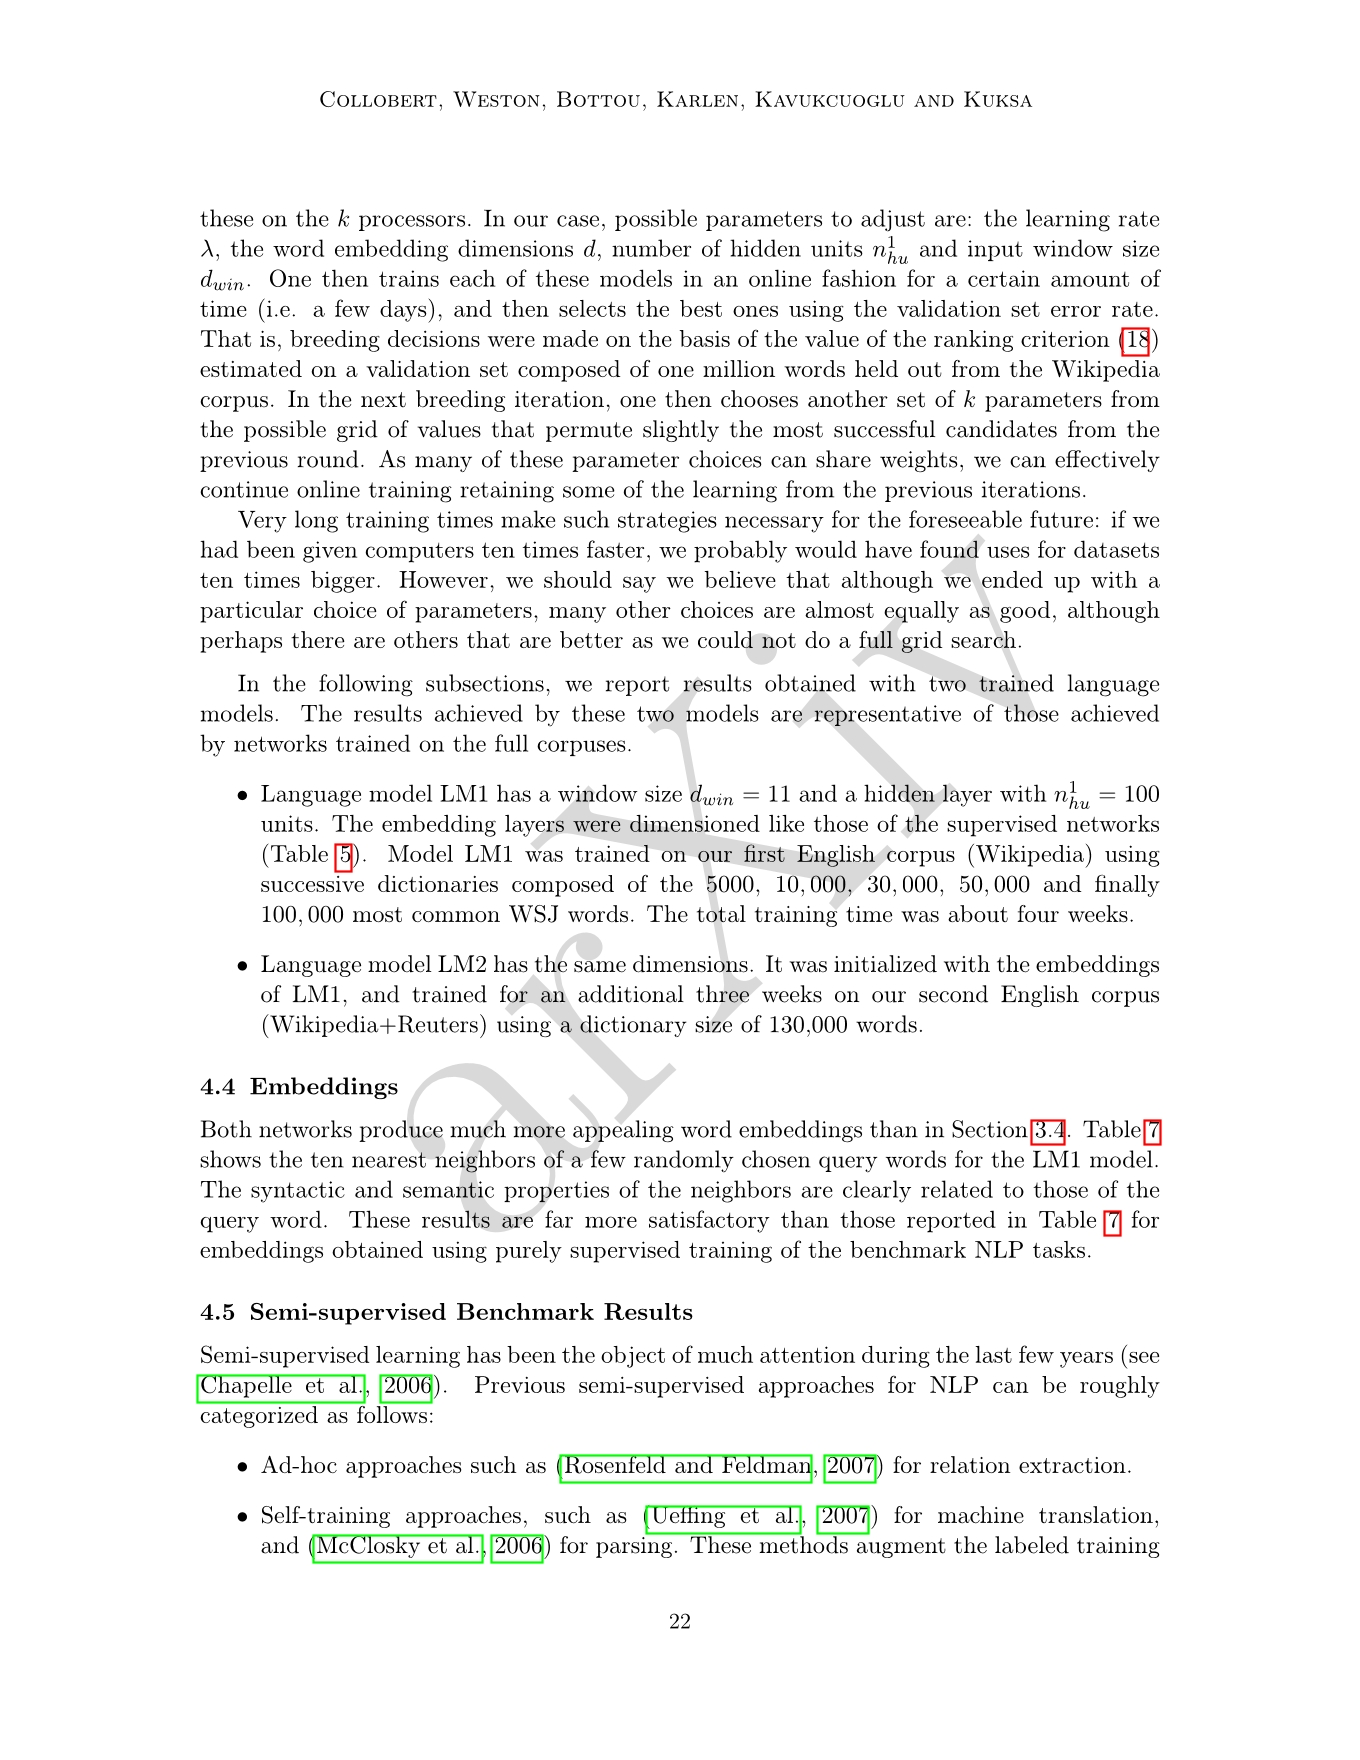
\includegraphics[width=\textwidth]{translations/collobert_2011-22.jpg}
\end{center}
\begin{center}
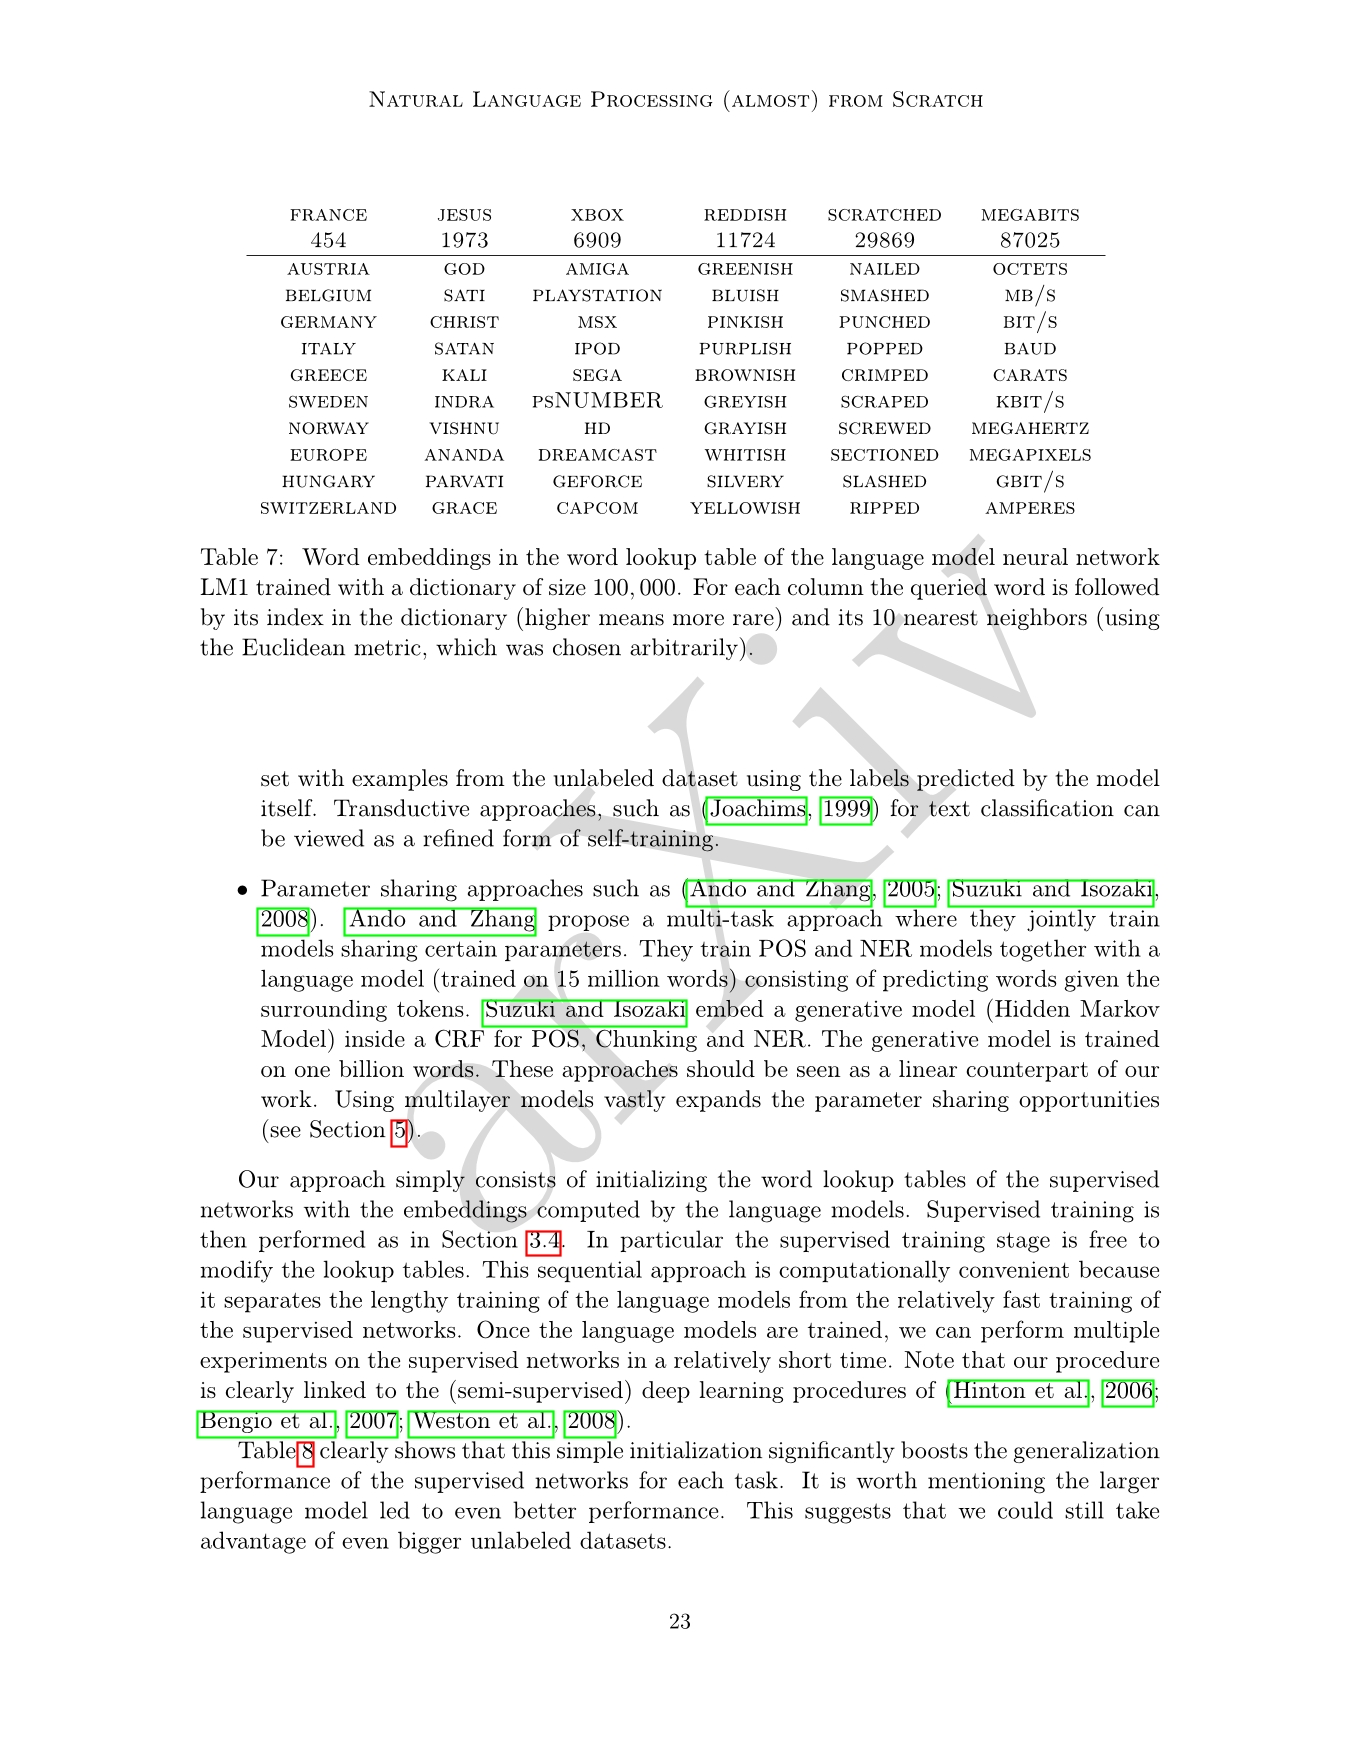
\includegraphics[width=\textwidth]{translations/collobert_2011-23.jpg}
\end{center}
\begin{center}
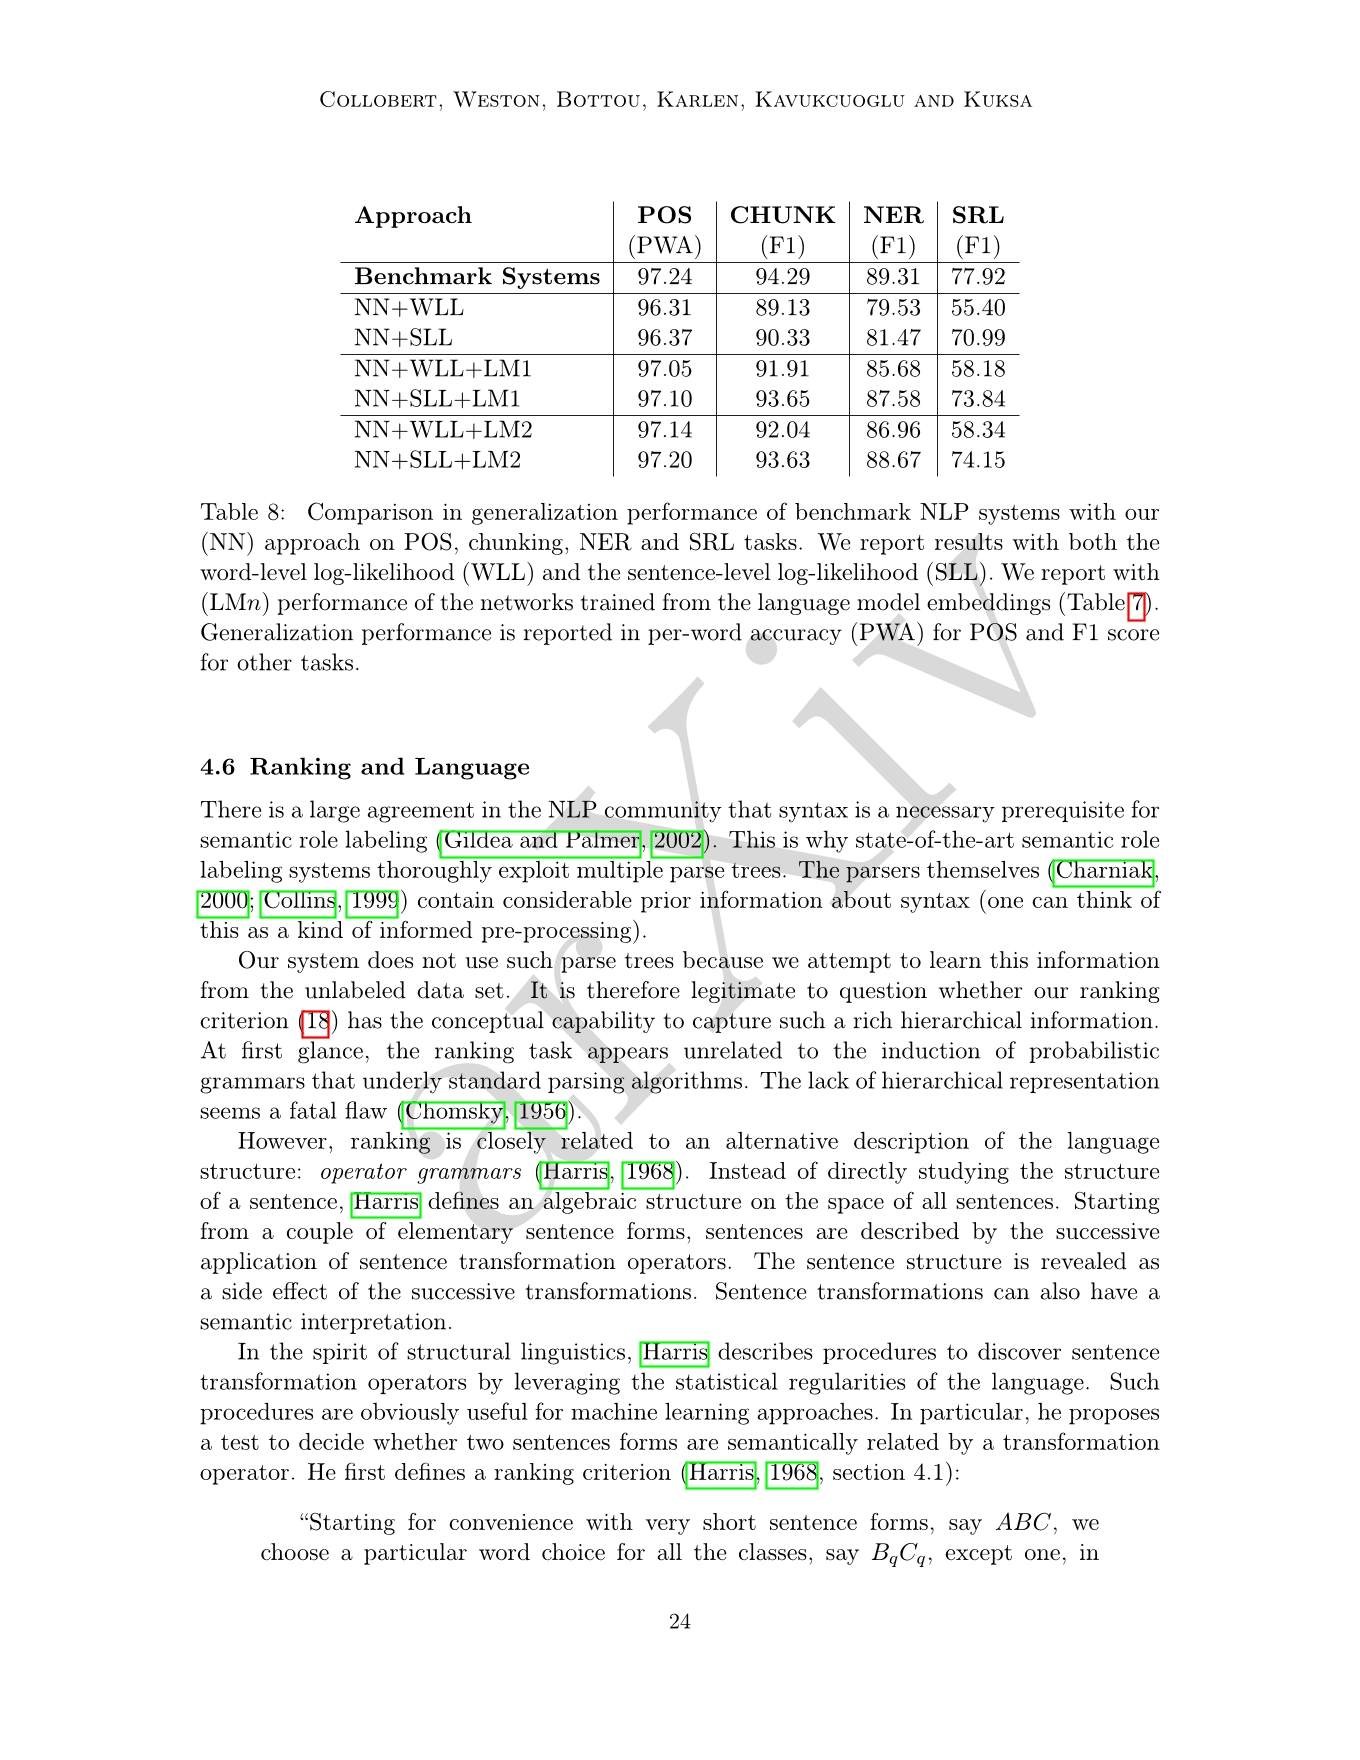
\includegraphics[width=\textwidth]{translations/collobert_2011-24.jpg}
\end{center}
\begin{center}
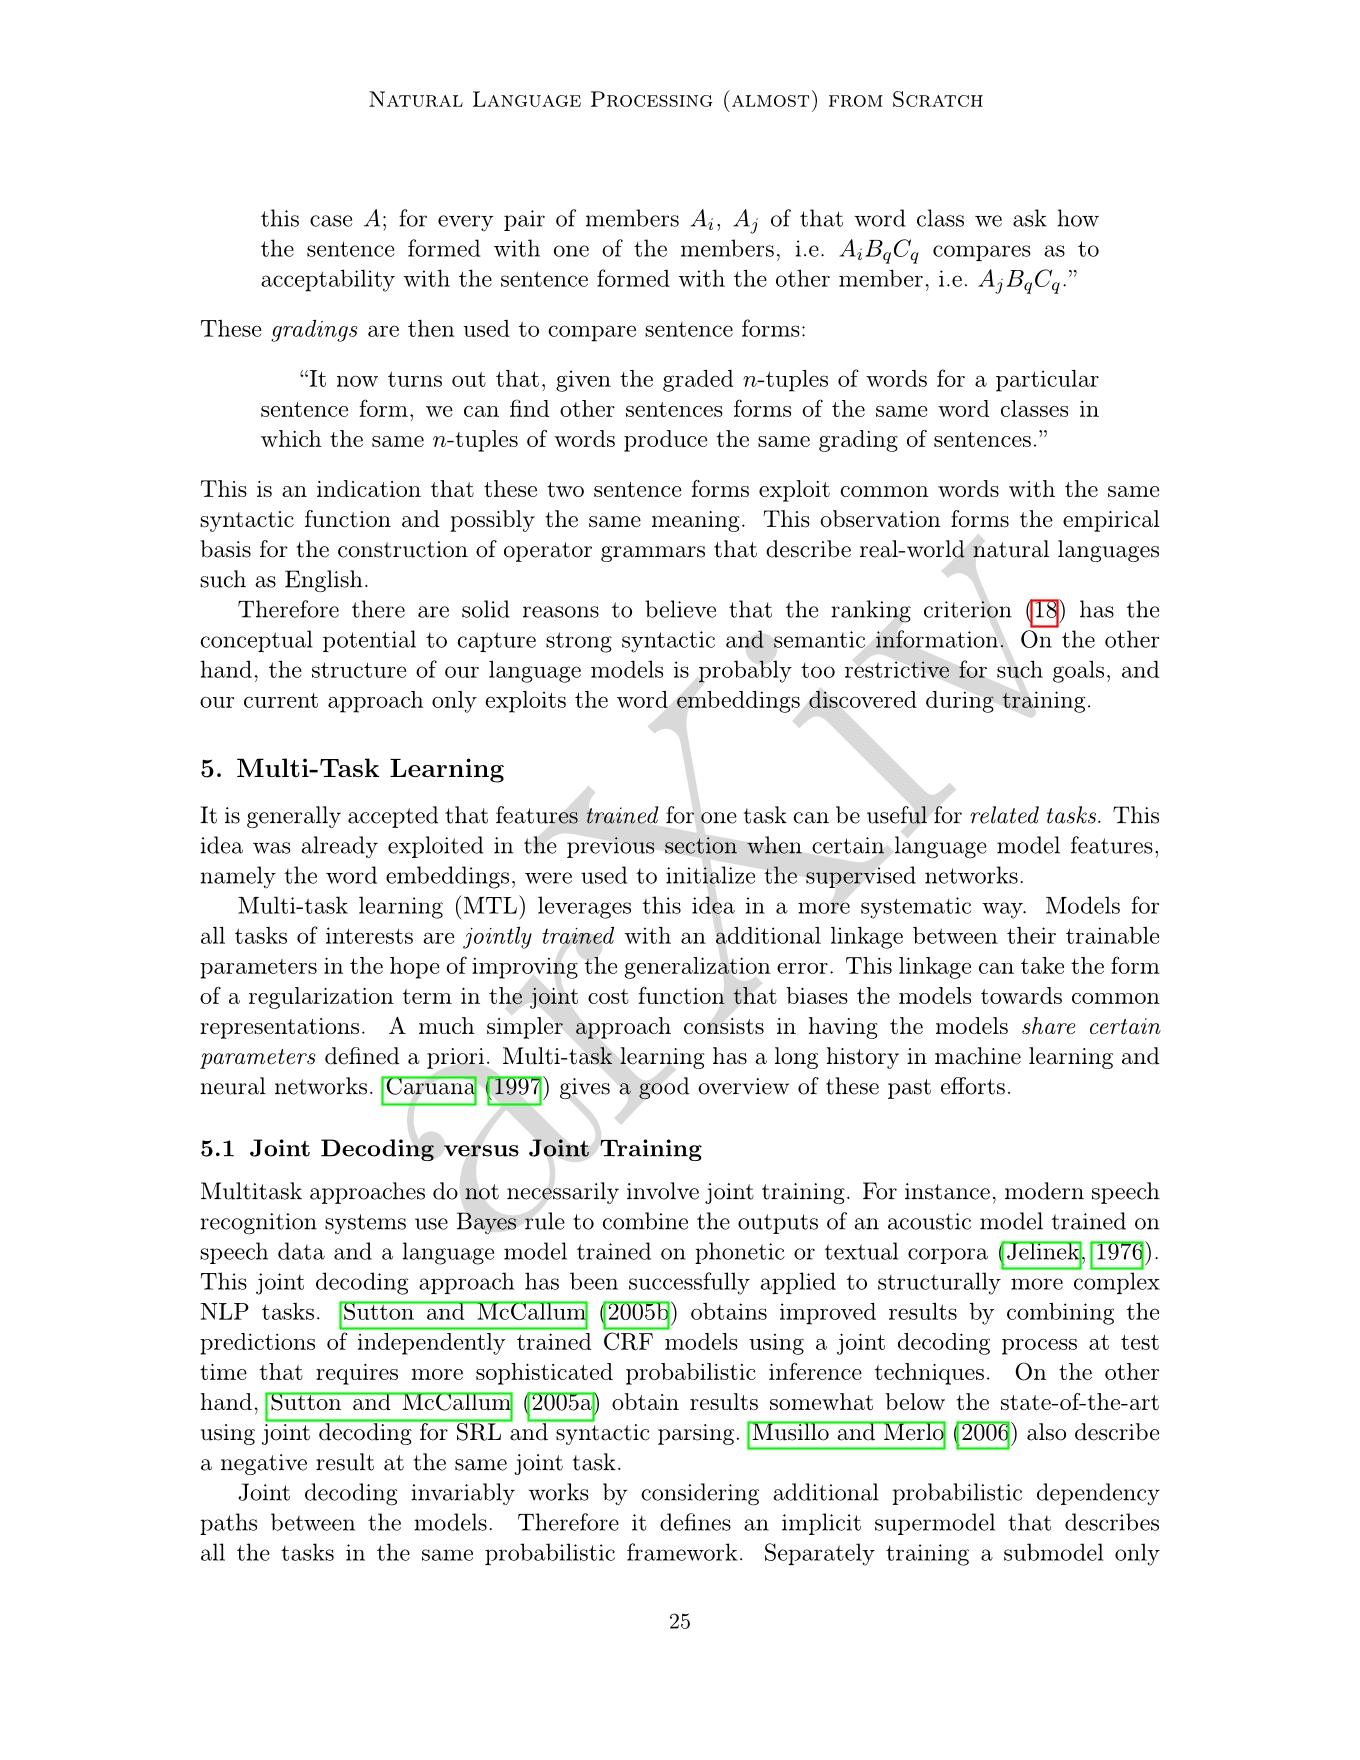
\includegraphics[width=\textwidth]{translations/collobert_2011-25.jpg}
\end{center}
\begin{center}
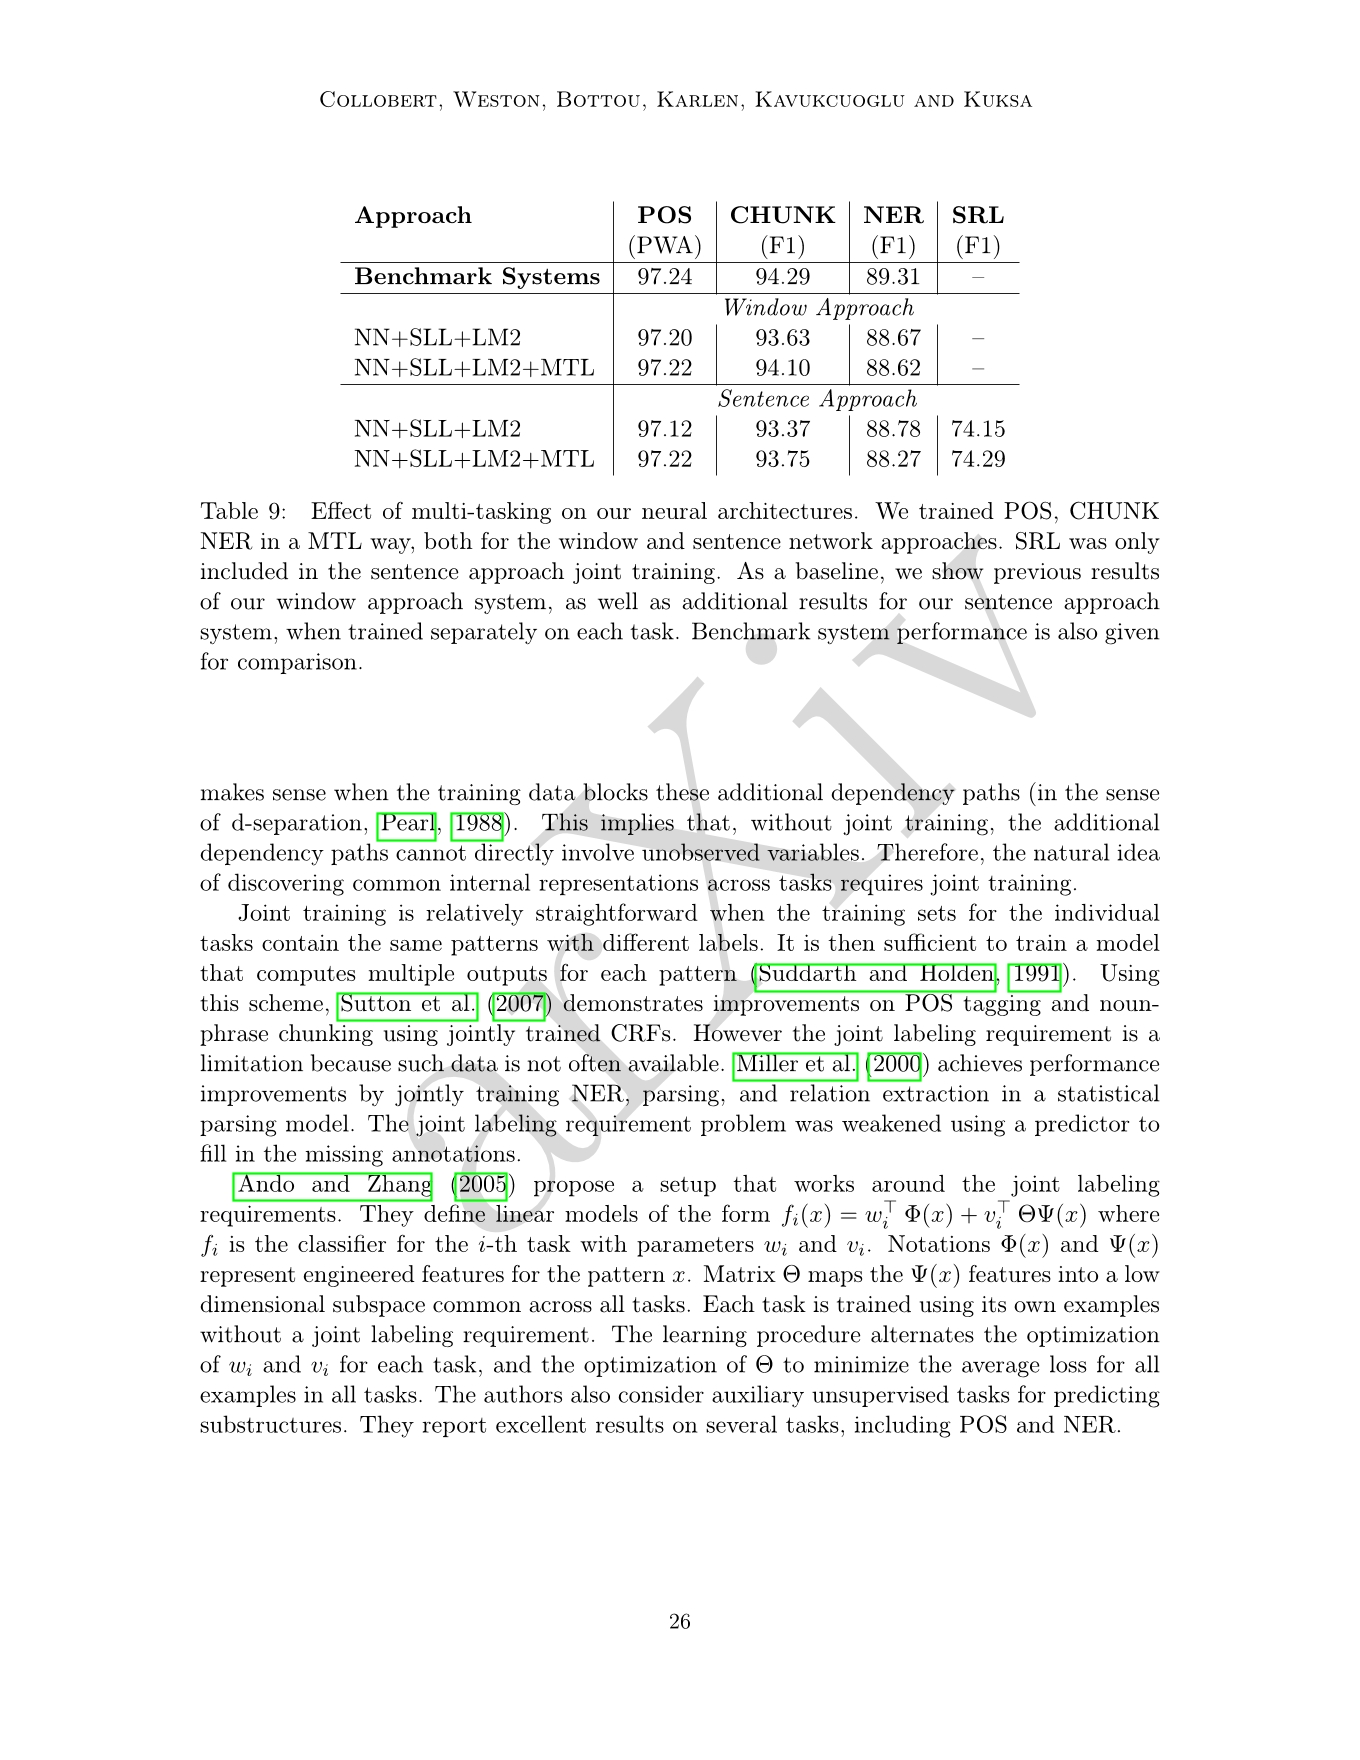
\includegraphics[width=\textwidth]{translations/collobert_2011-26.jpg}
\end{center}
\begin{center}
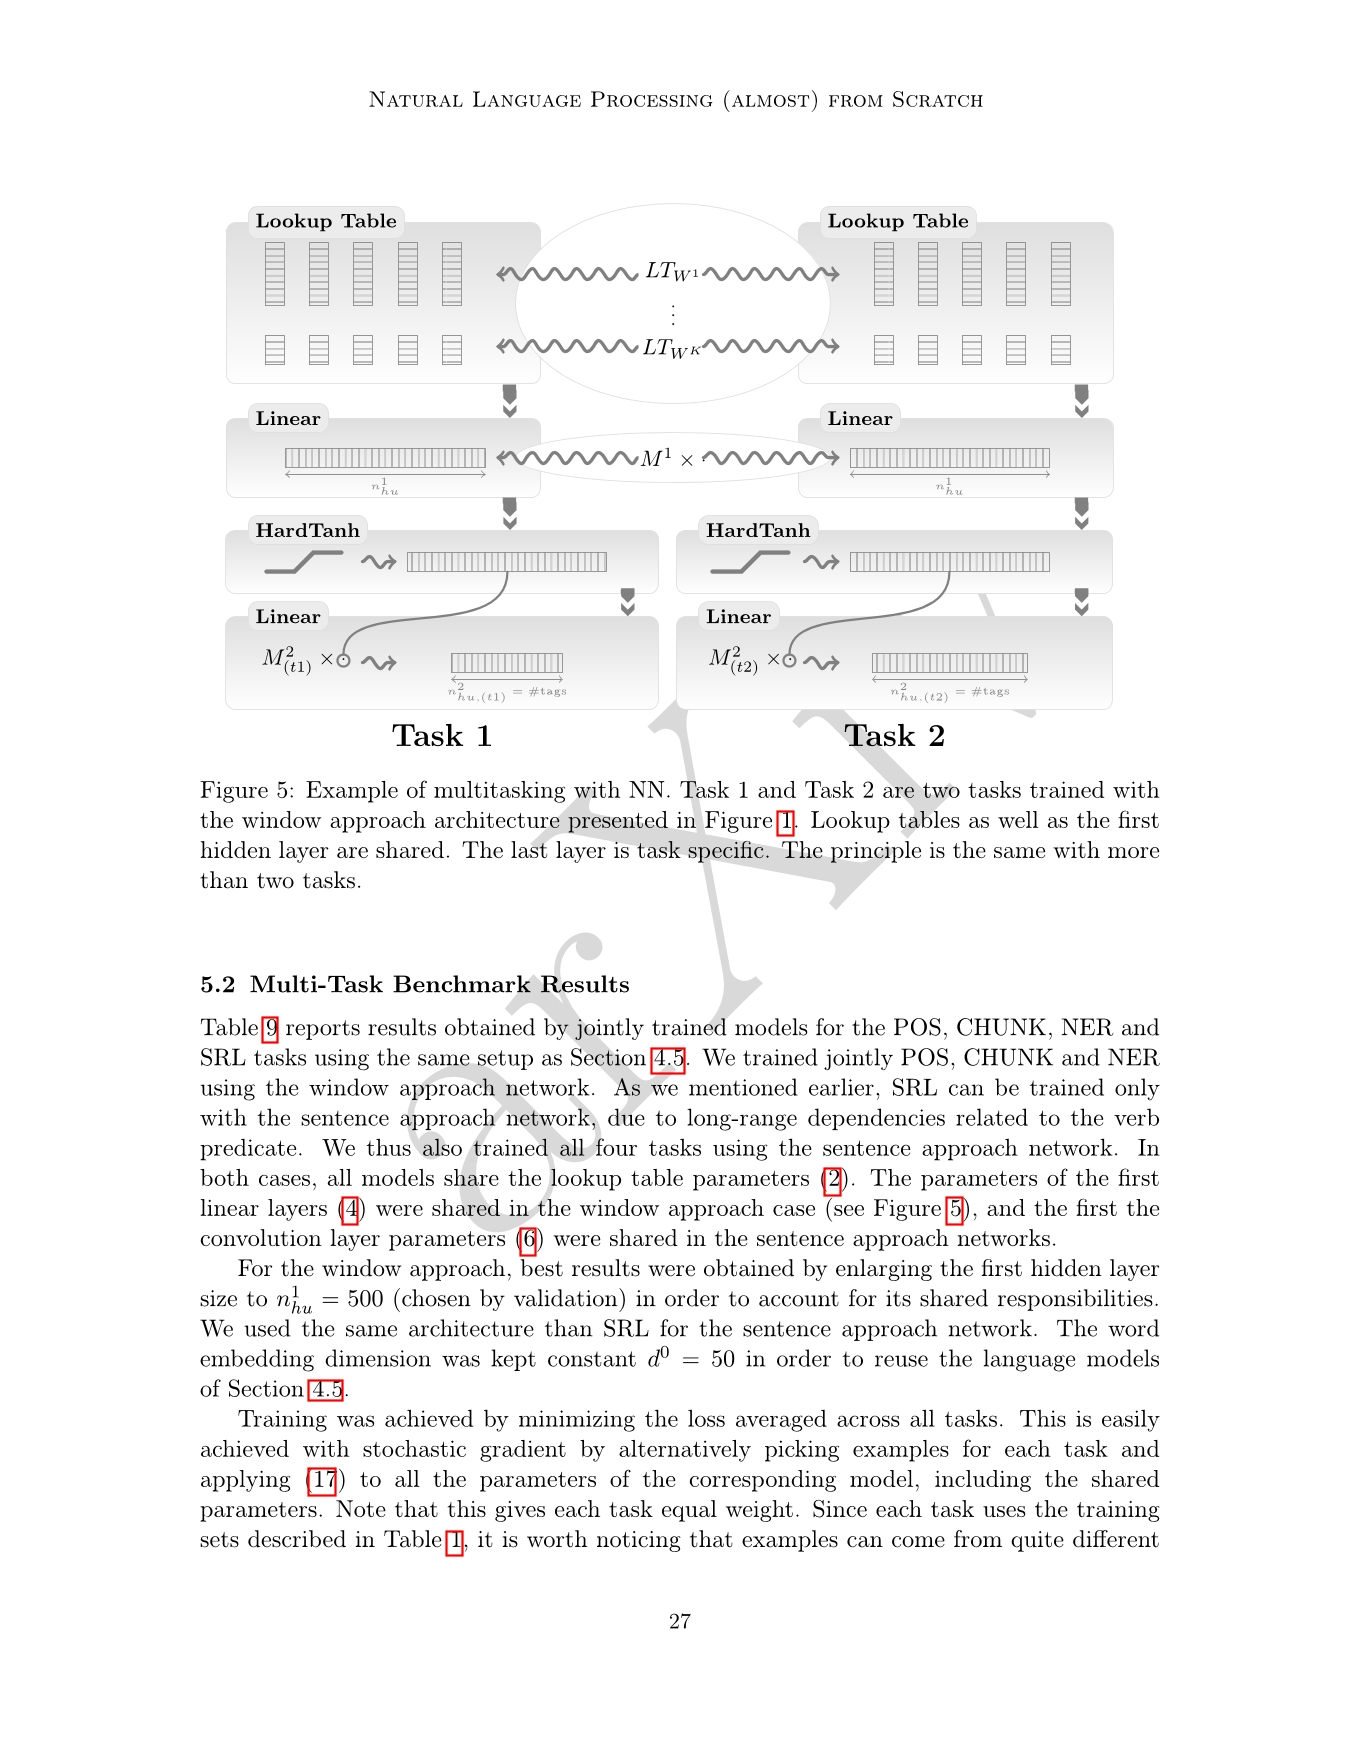
\includegraphics[width=\textwidth]{translations/collobert_2011-27.jpg}
\end{center}
\begin{center}
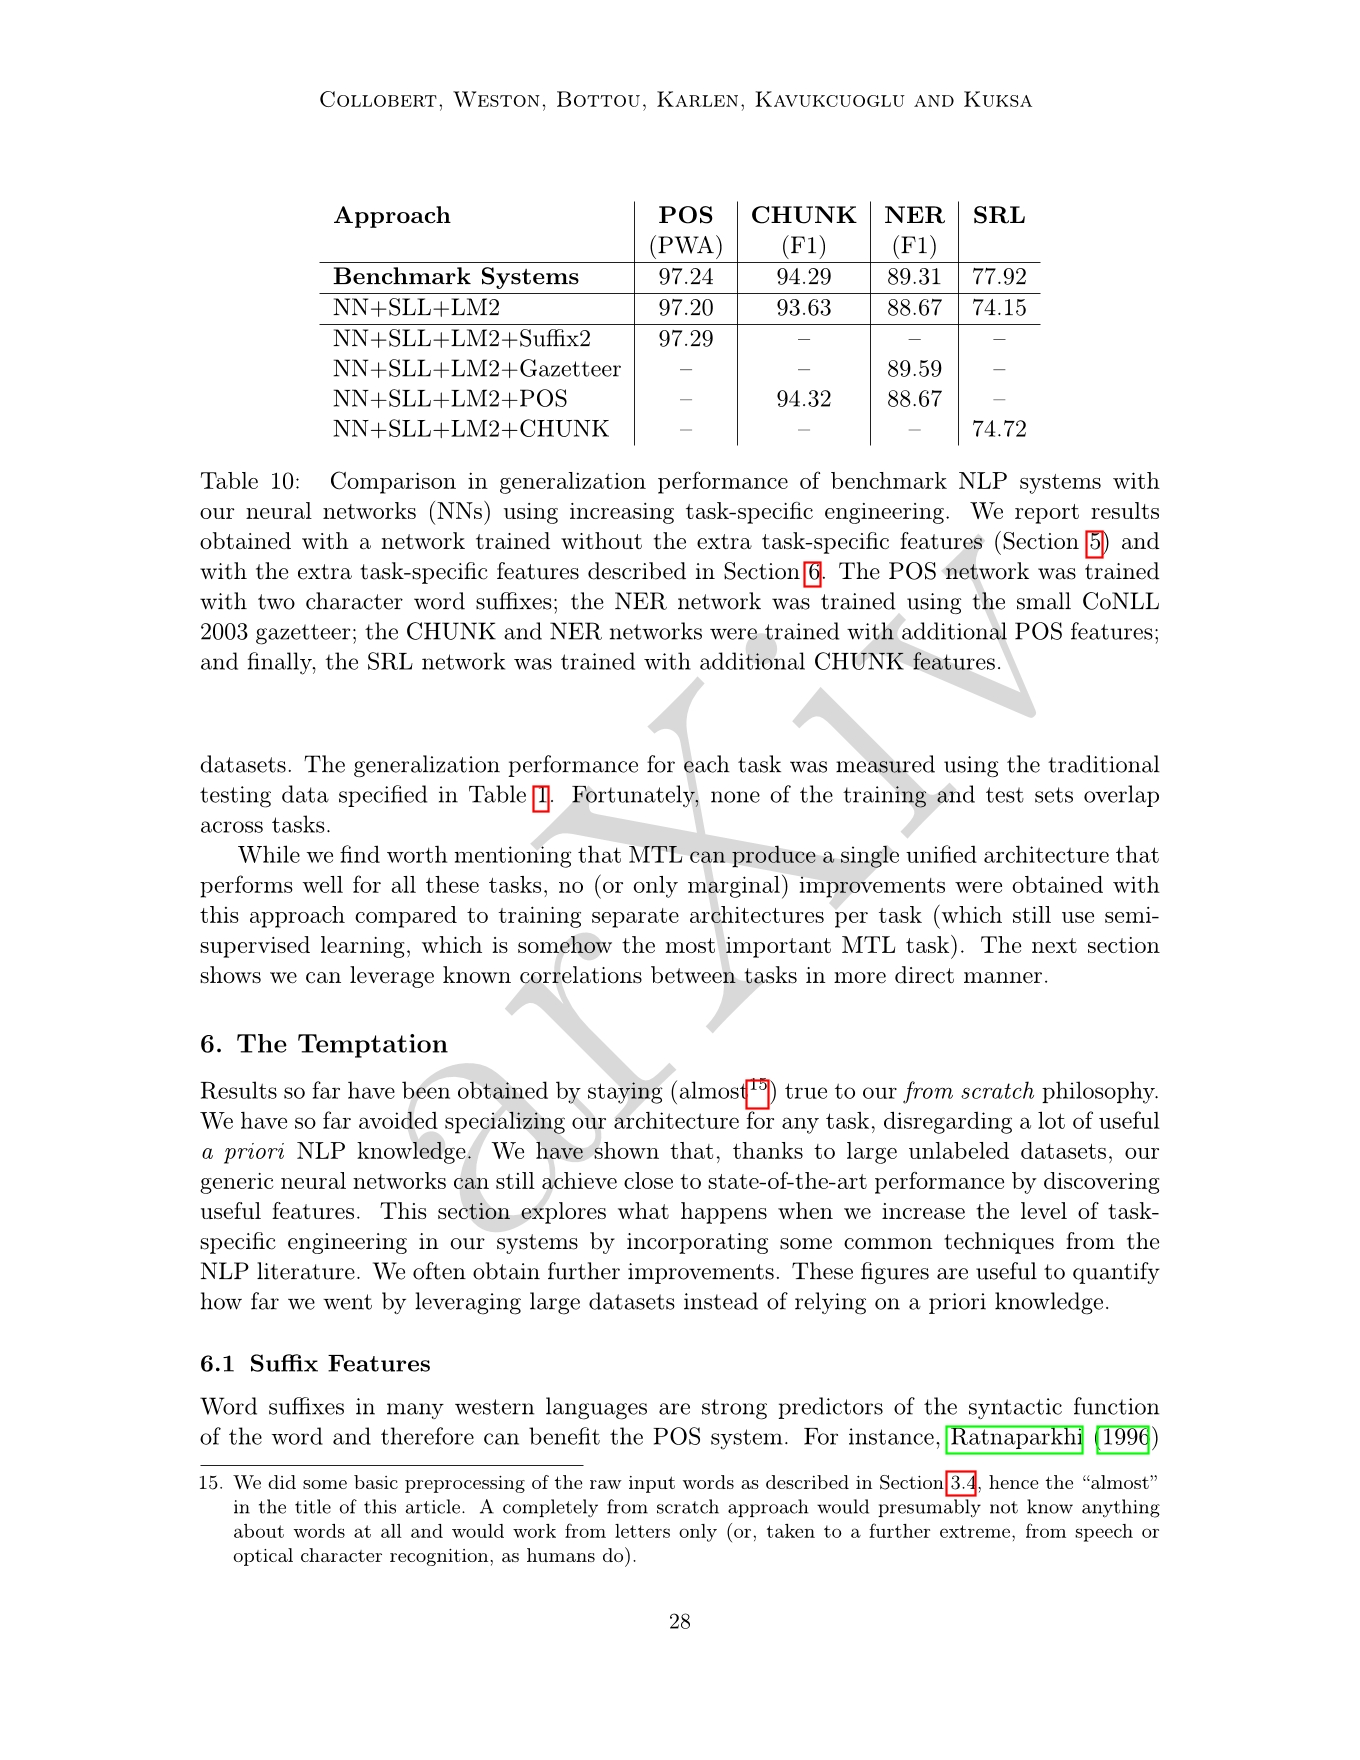
\includegraphics[width=\textwidth]{translations/collobert_2011-28.jpg}
\end{center}
\begin{center}
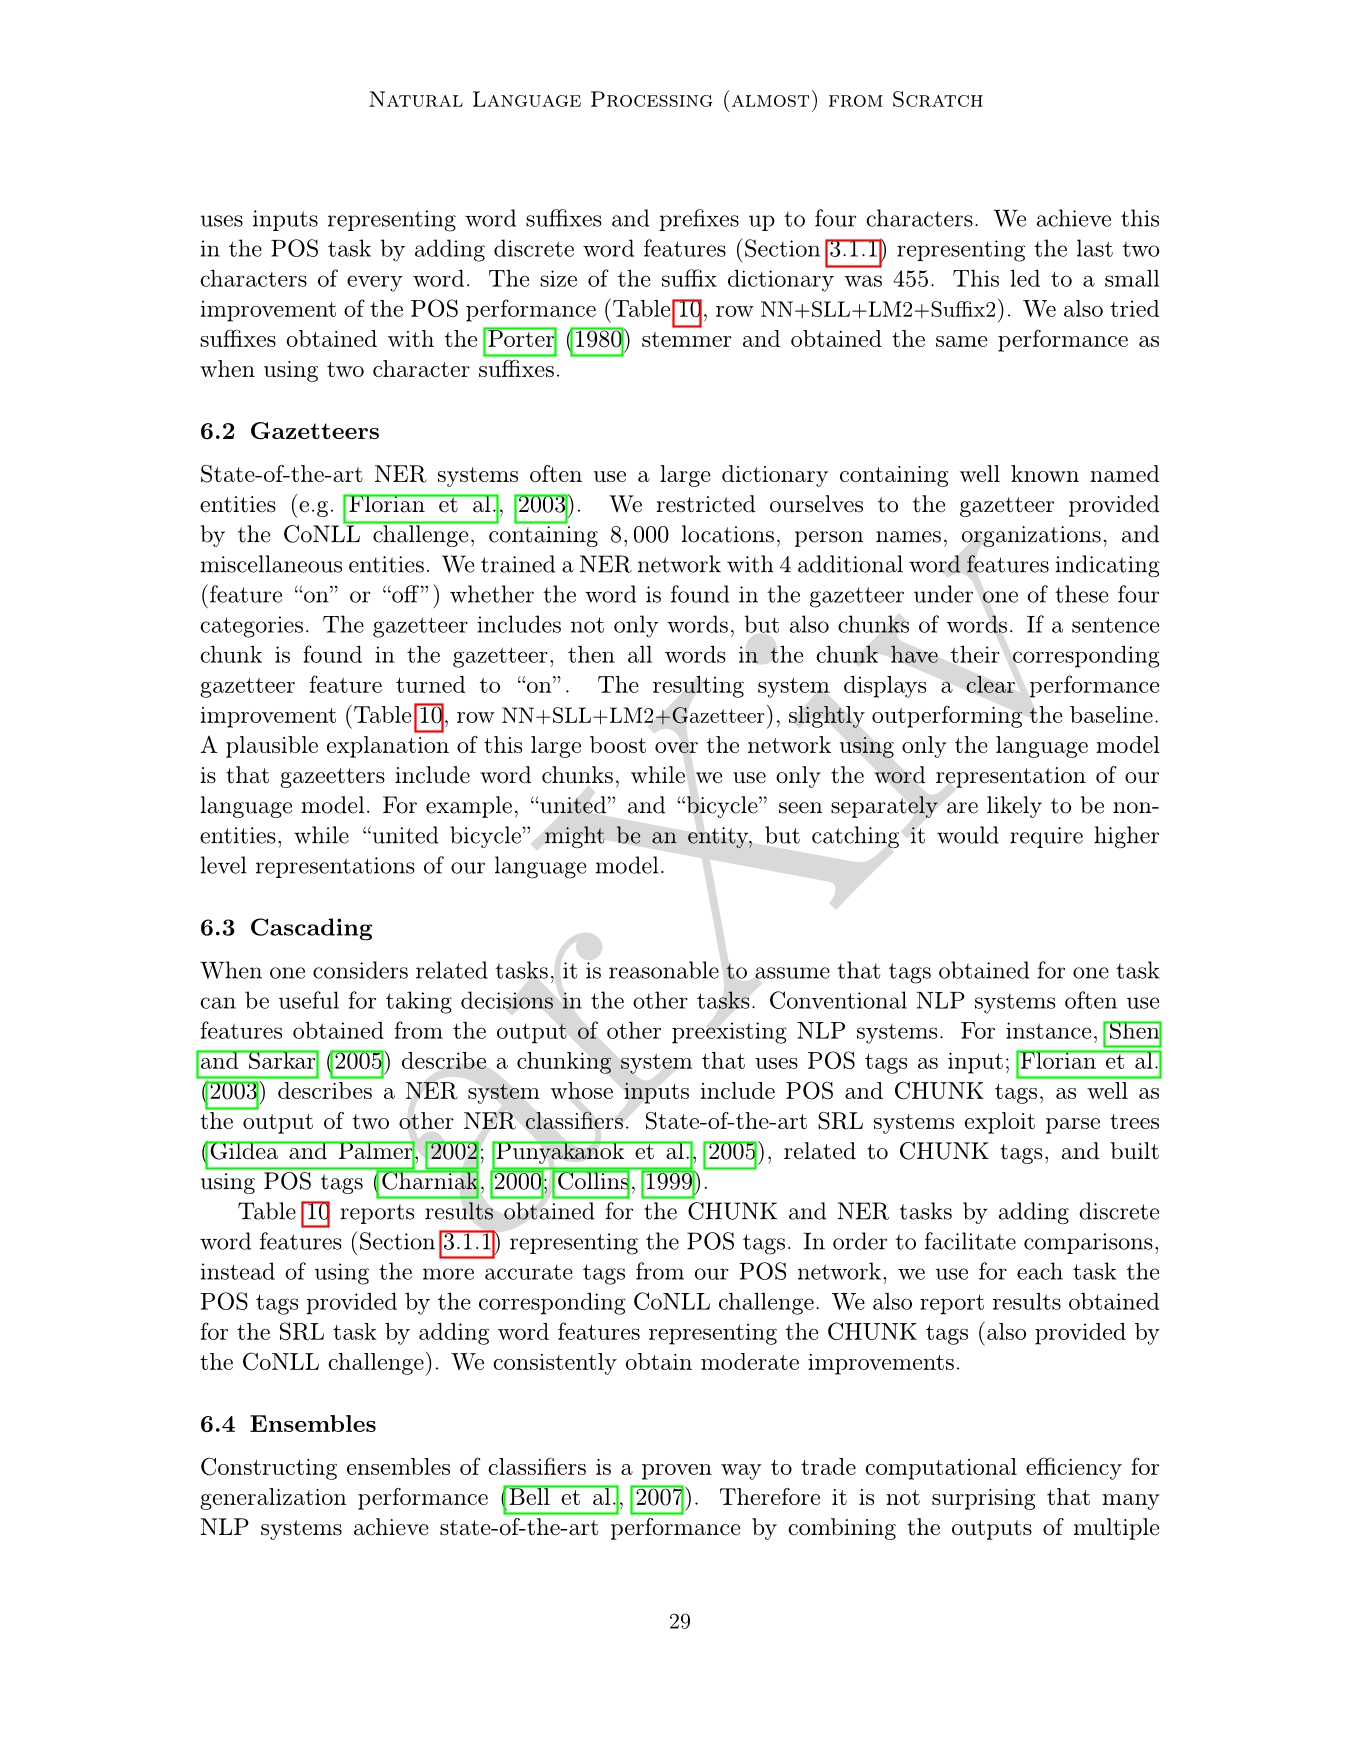
\includegraphics[width=\textwidth]{translations/collobert_2011-29.jpg}
\end{center}
\begin{center}
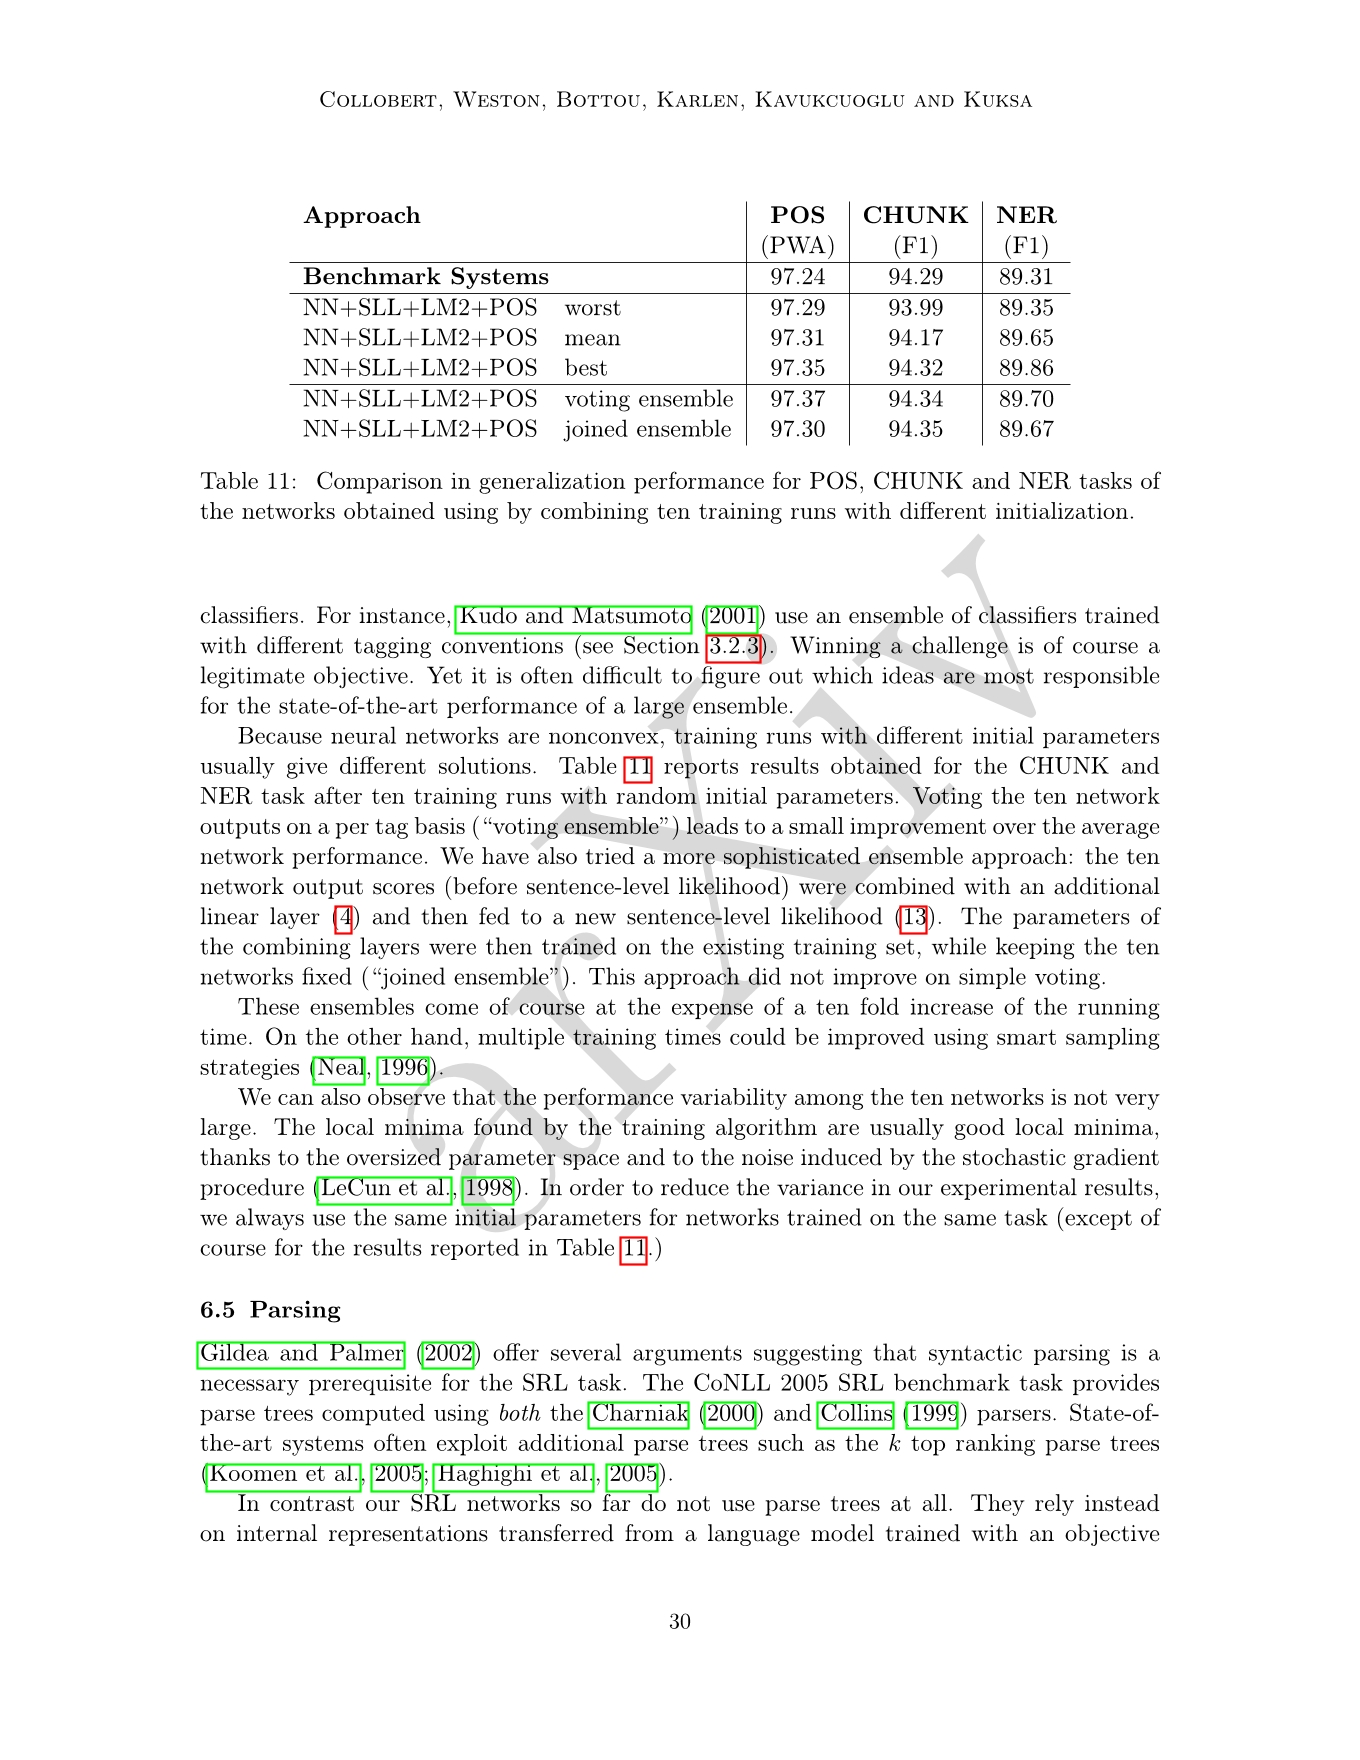
\includegraphics[width=\textwidth]{translations/collobert_2011-30.jpg}
\end{center}
\begin{center}
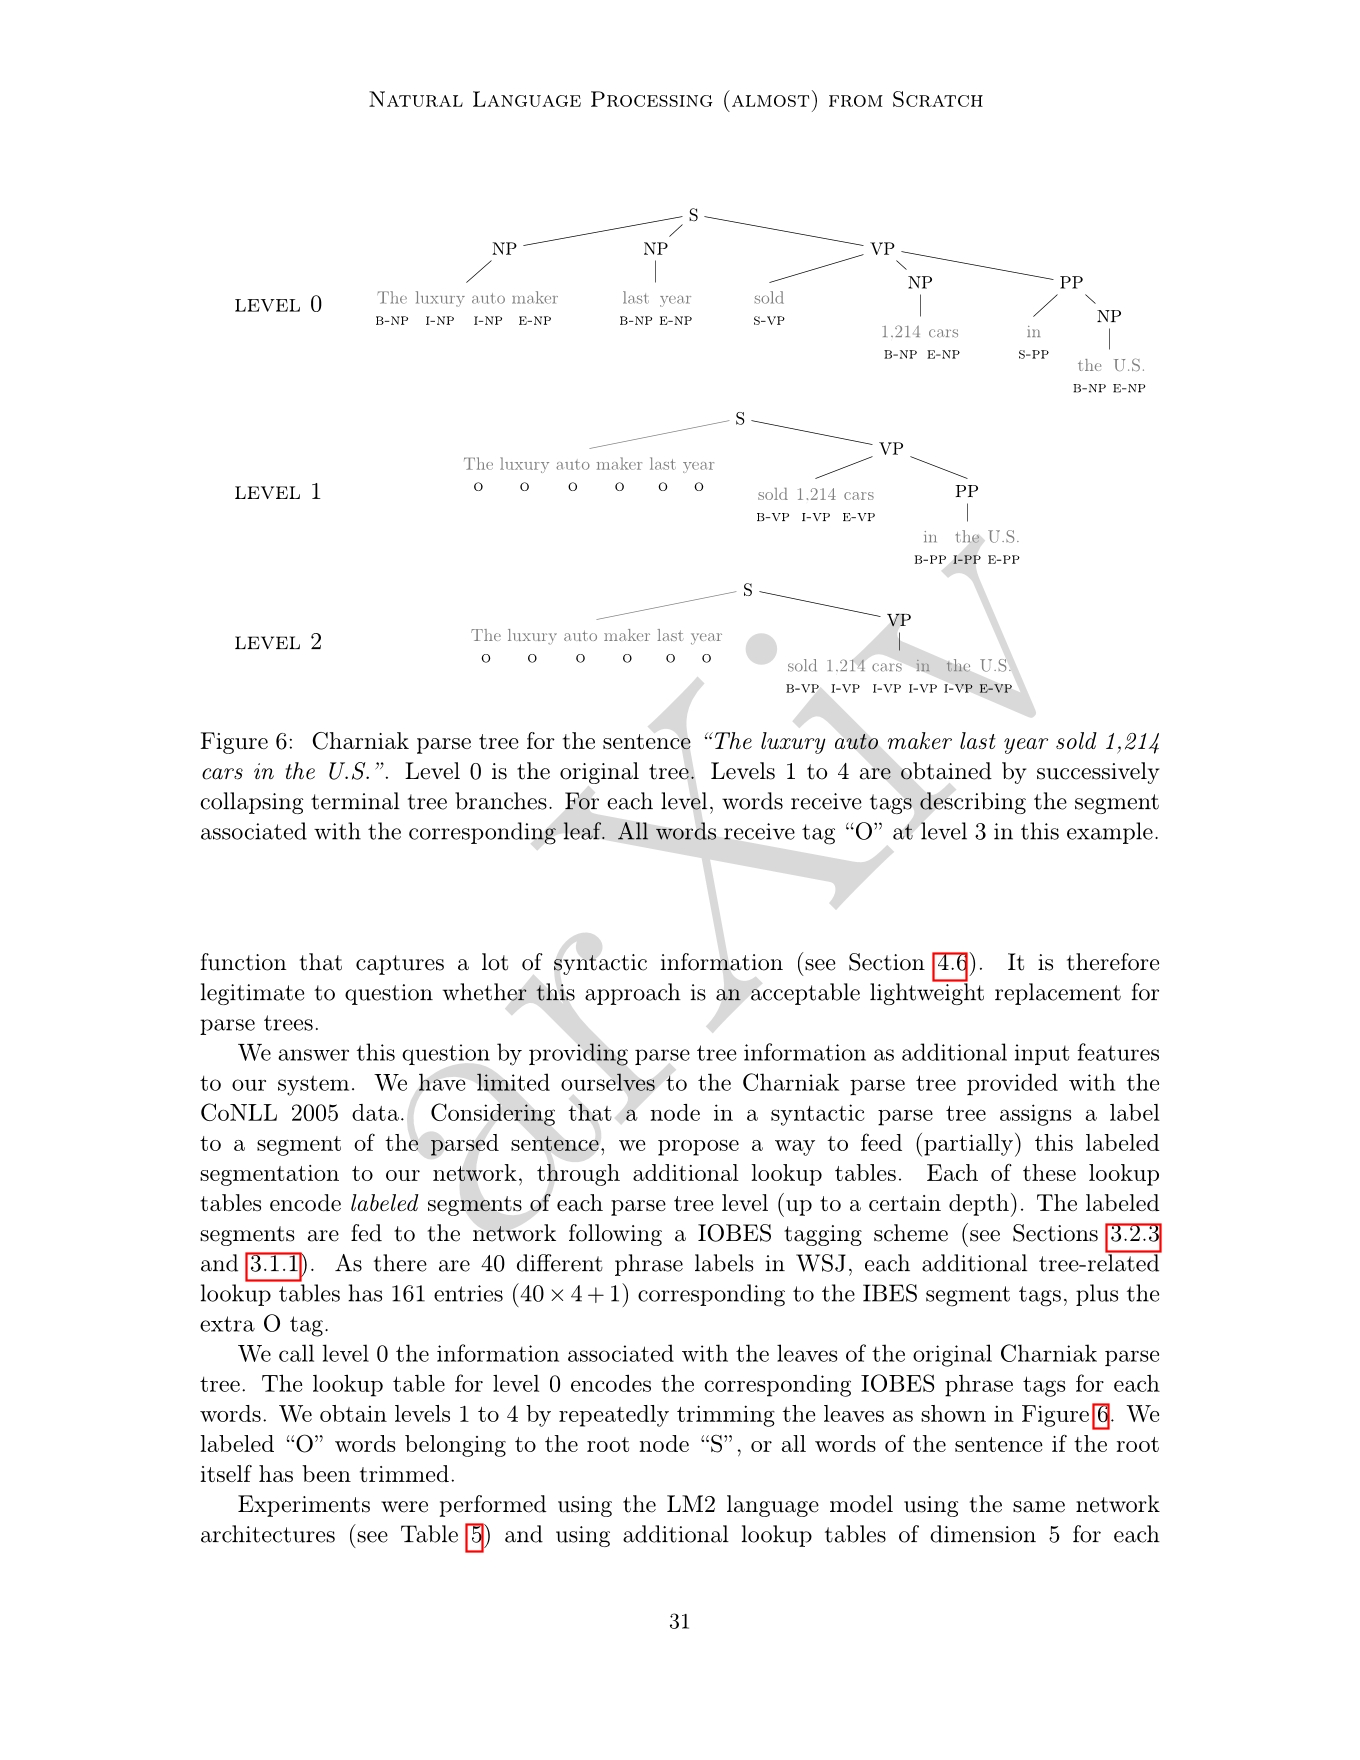
\includegraphics[width=\textwidth]{translations/collobert_2011-31.jpg}
\end{center}
\begin{center}
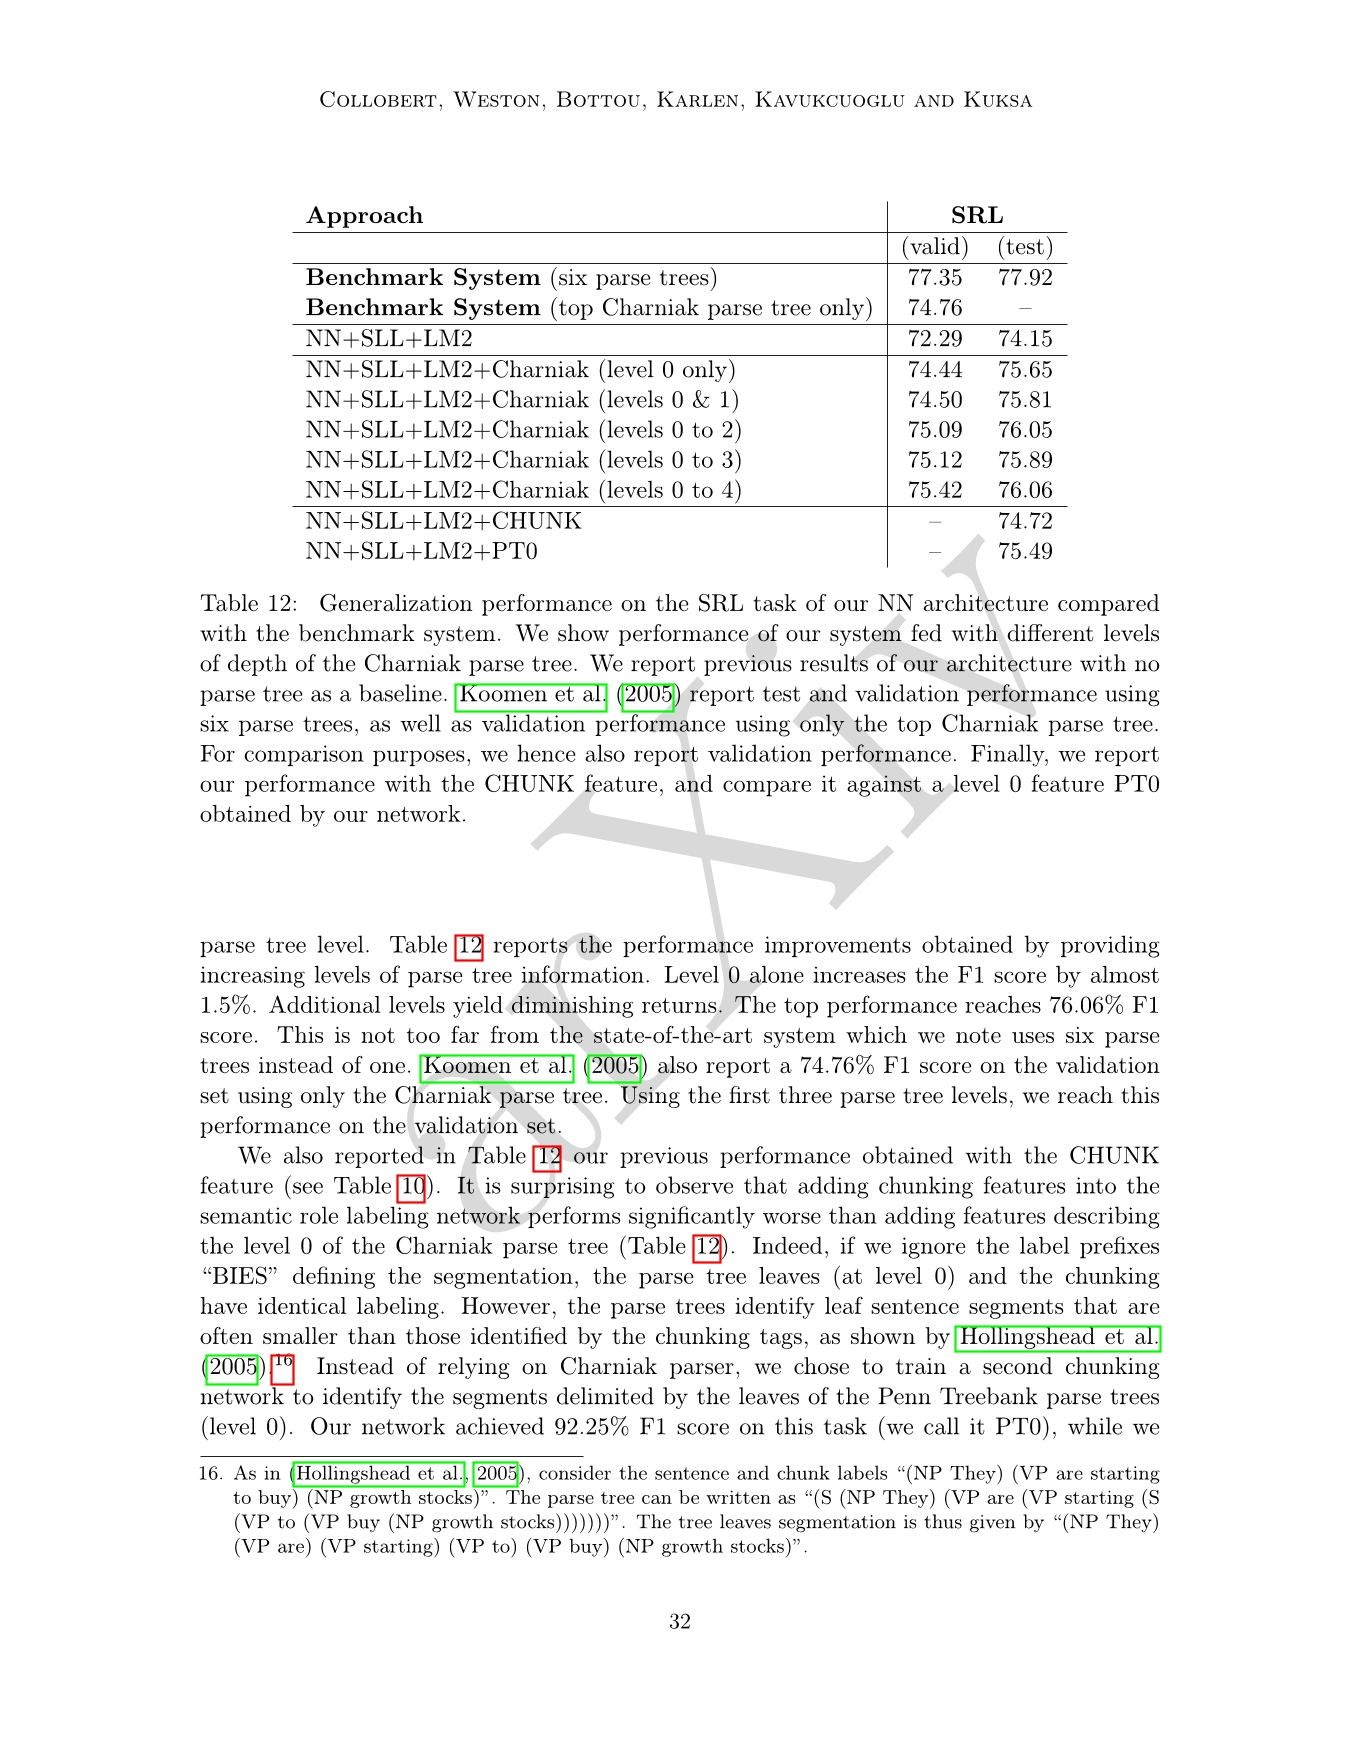
\includegraphics[width=\textwidth]{translations/collobert_2011-32.jpg}
\end{center}
\begin{center}
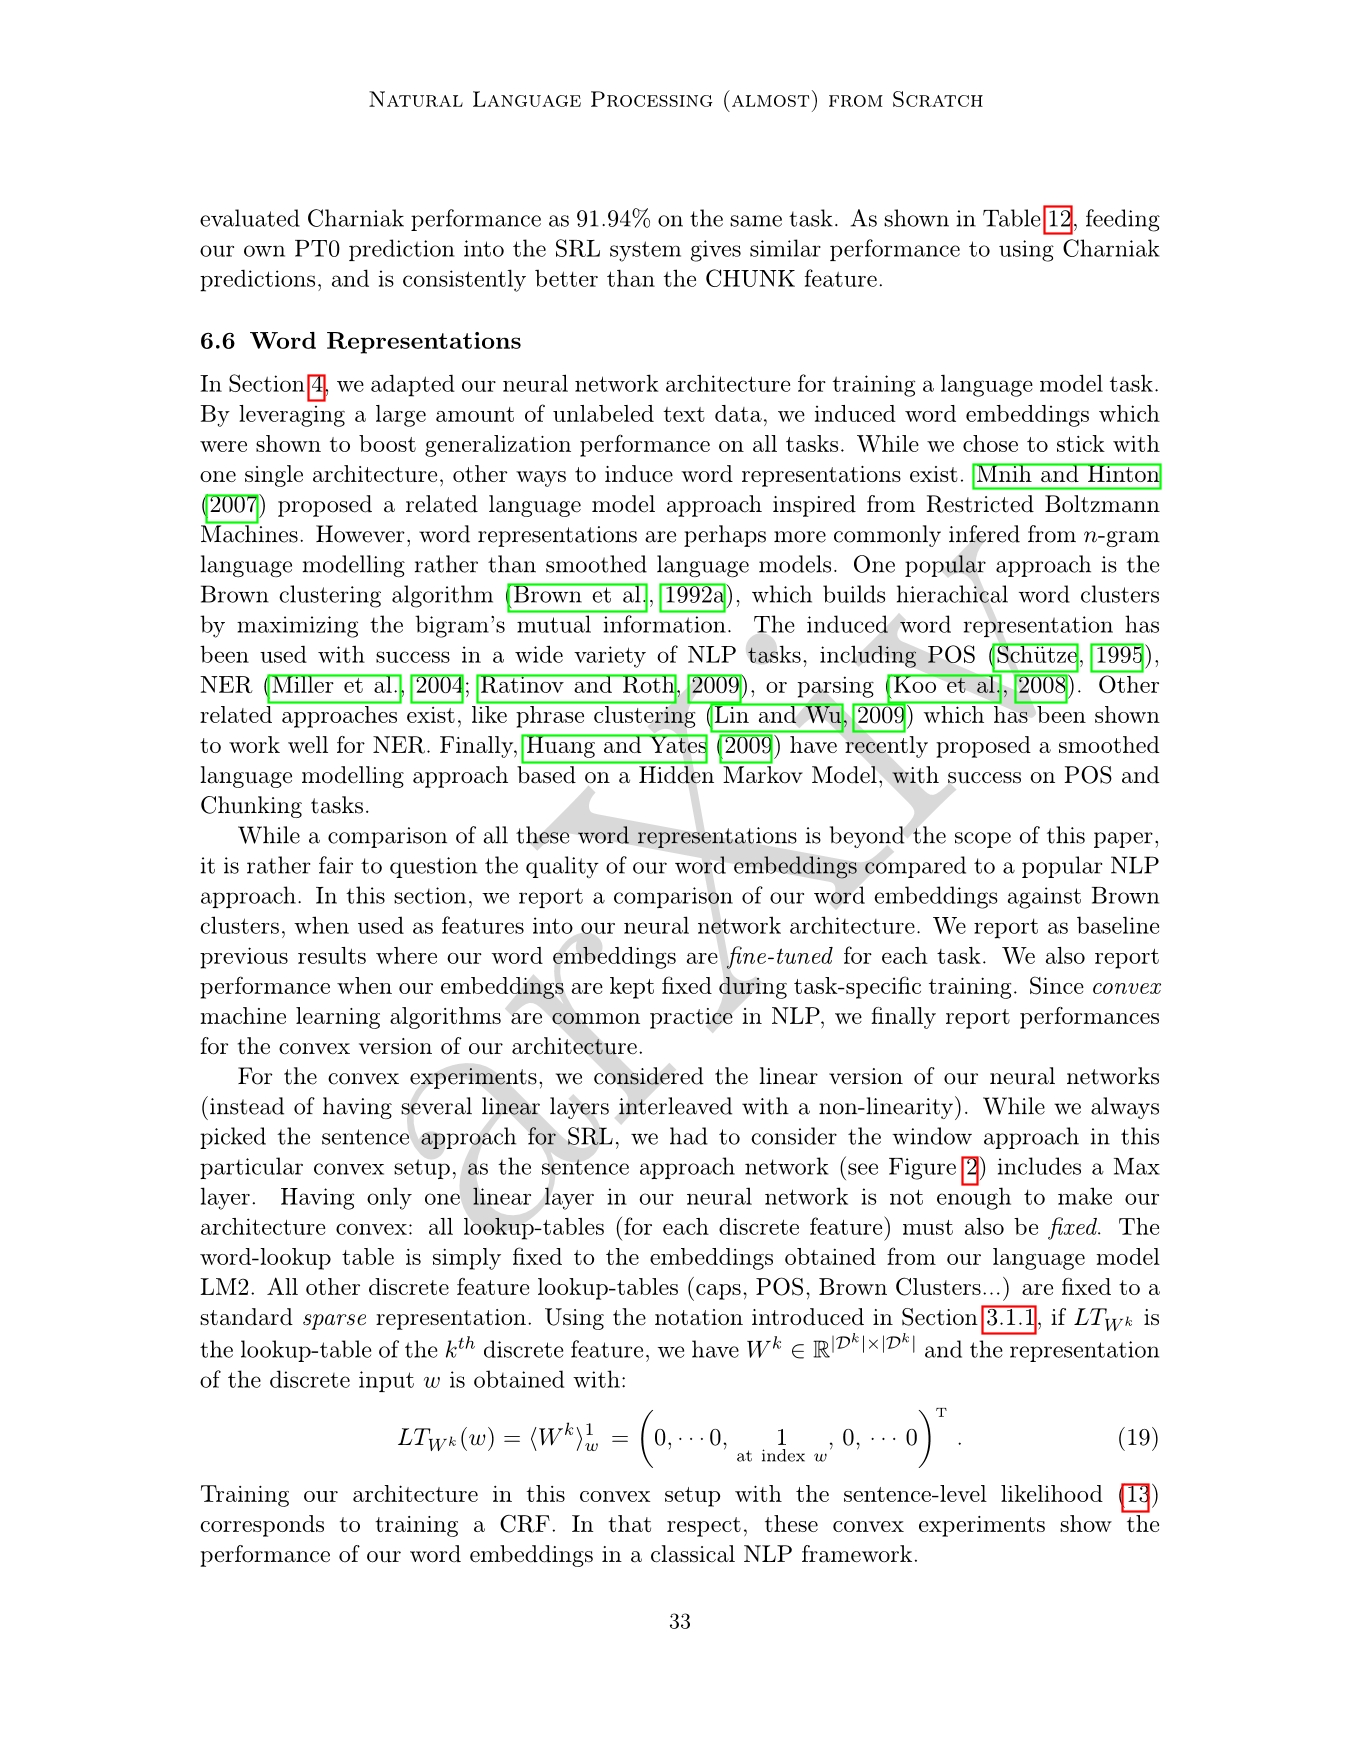
\includegraphics[width=\textwidth]{translations/collobert_2011-33.jpg}
\end{center}
\begin{center}
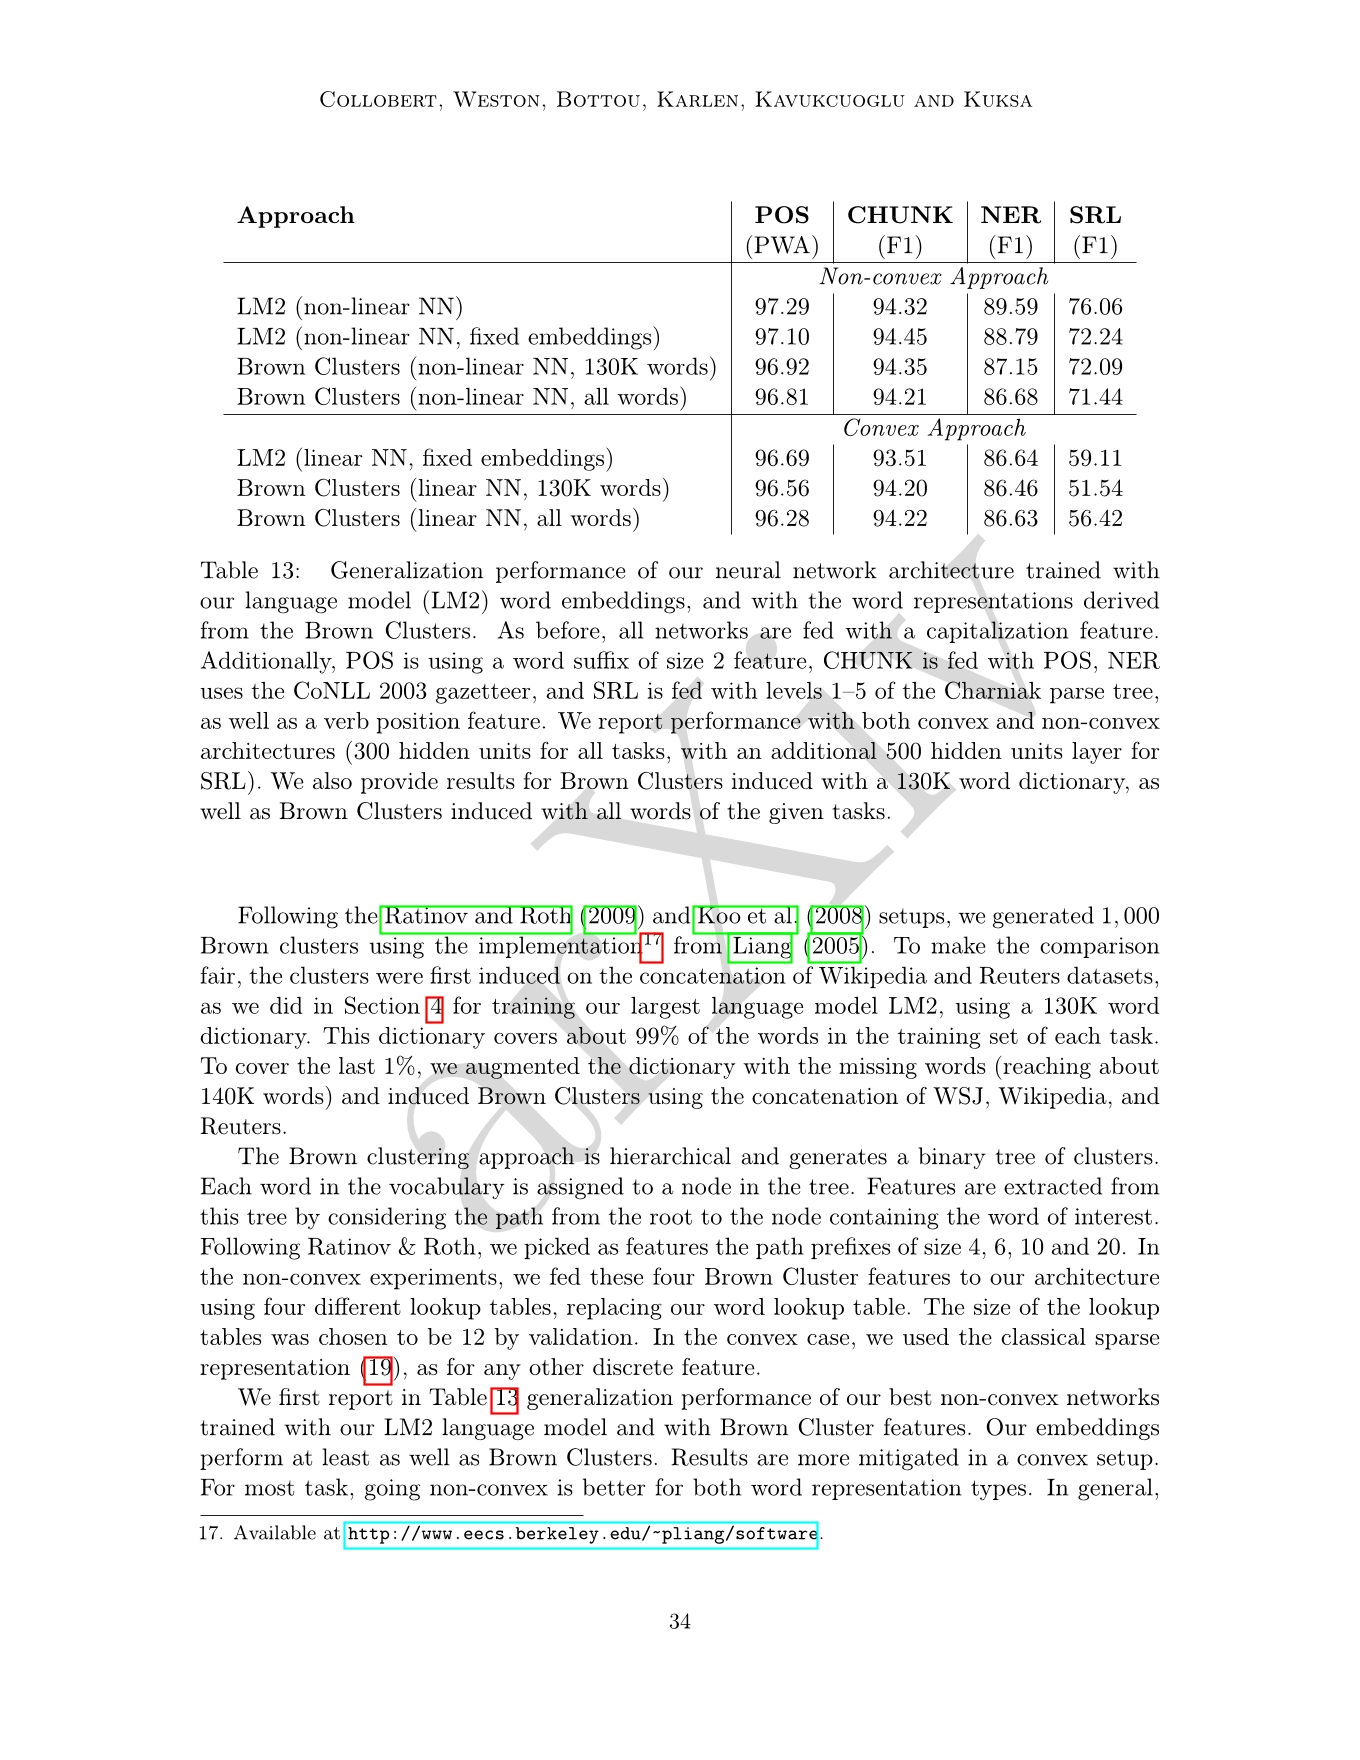
\includegraphics[width=\textwidth]{translations/collobert_2011-34.jpg}
\end{center}
\begin{center}
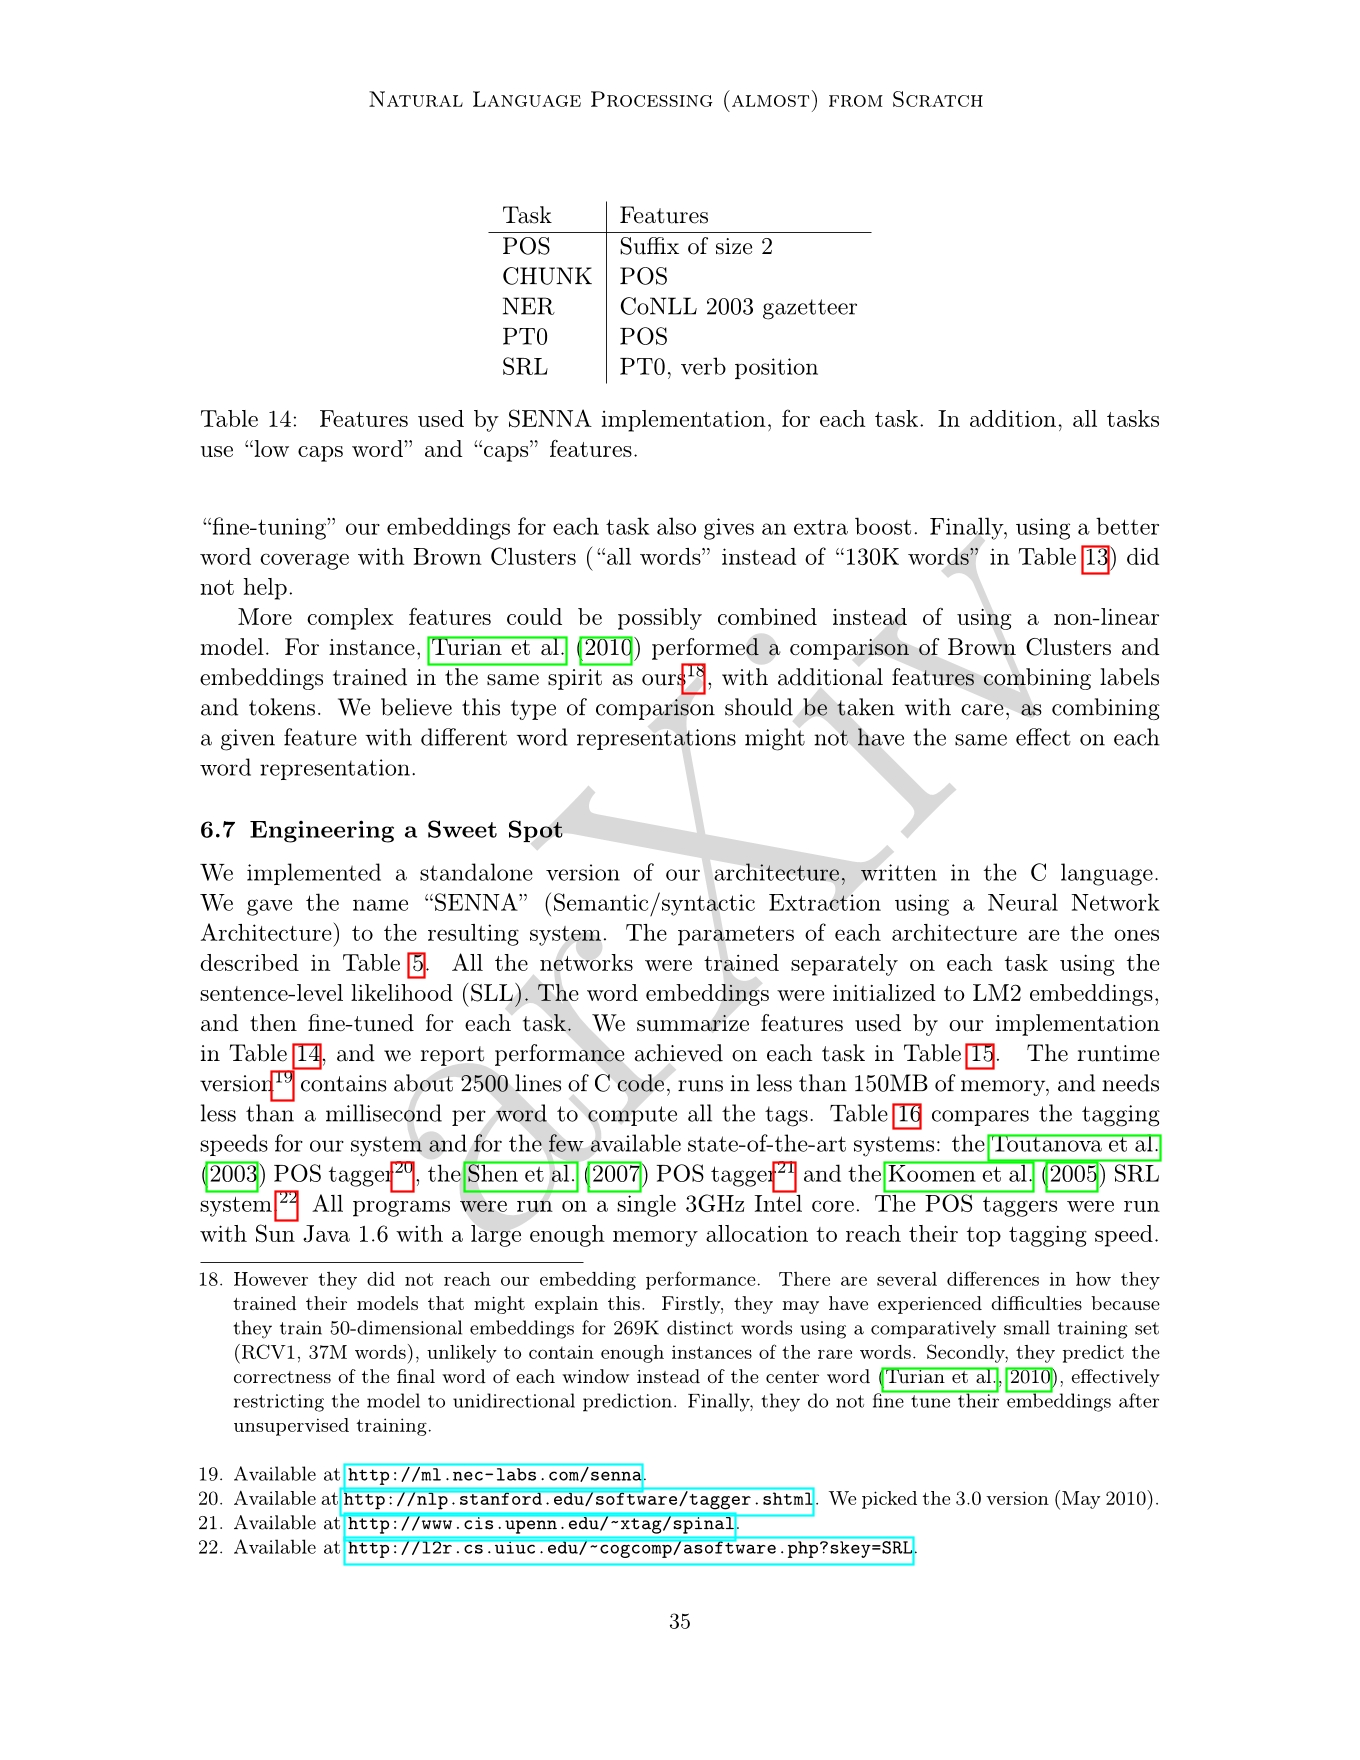
\includegraphics[width=\textwidth]{translations/collobert_2011-35.jpg}
\end{center}
\begin{center}
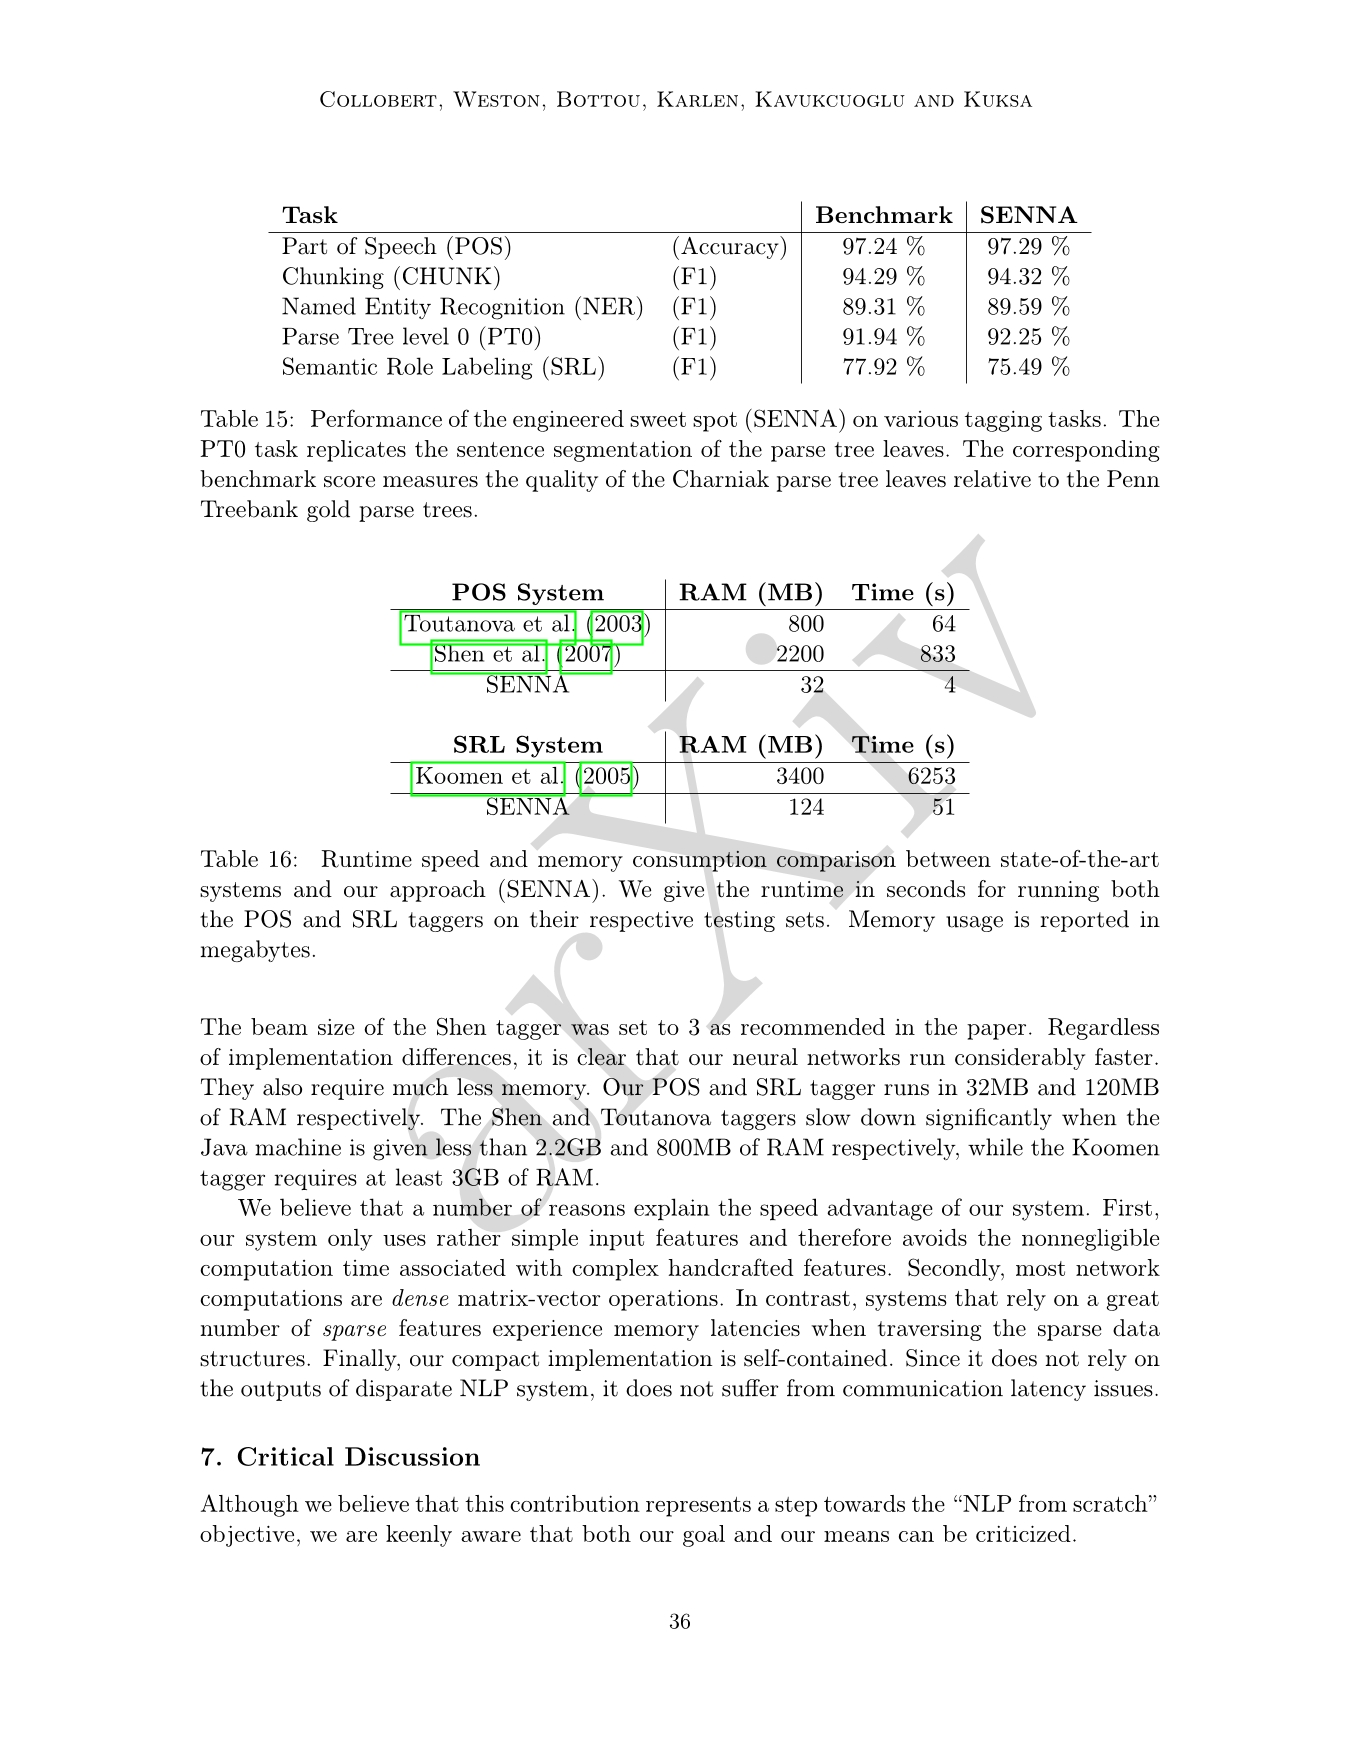
\includegraphics[width=\textwidth]{translations/collobert_2011-36.jpg}
\end{center}
\begin{center}
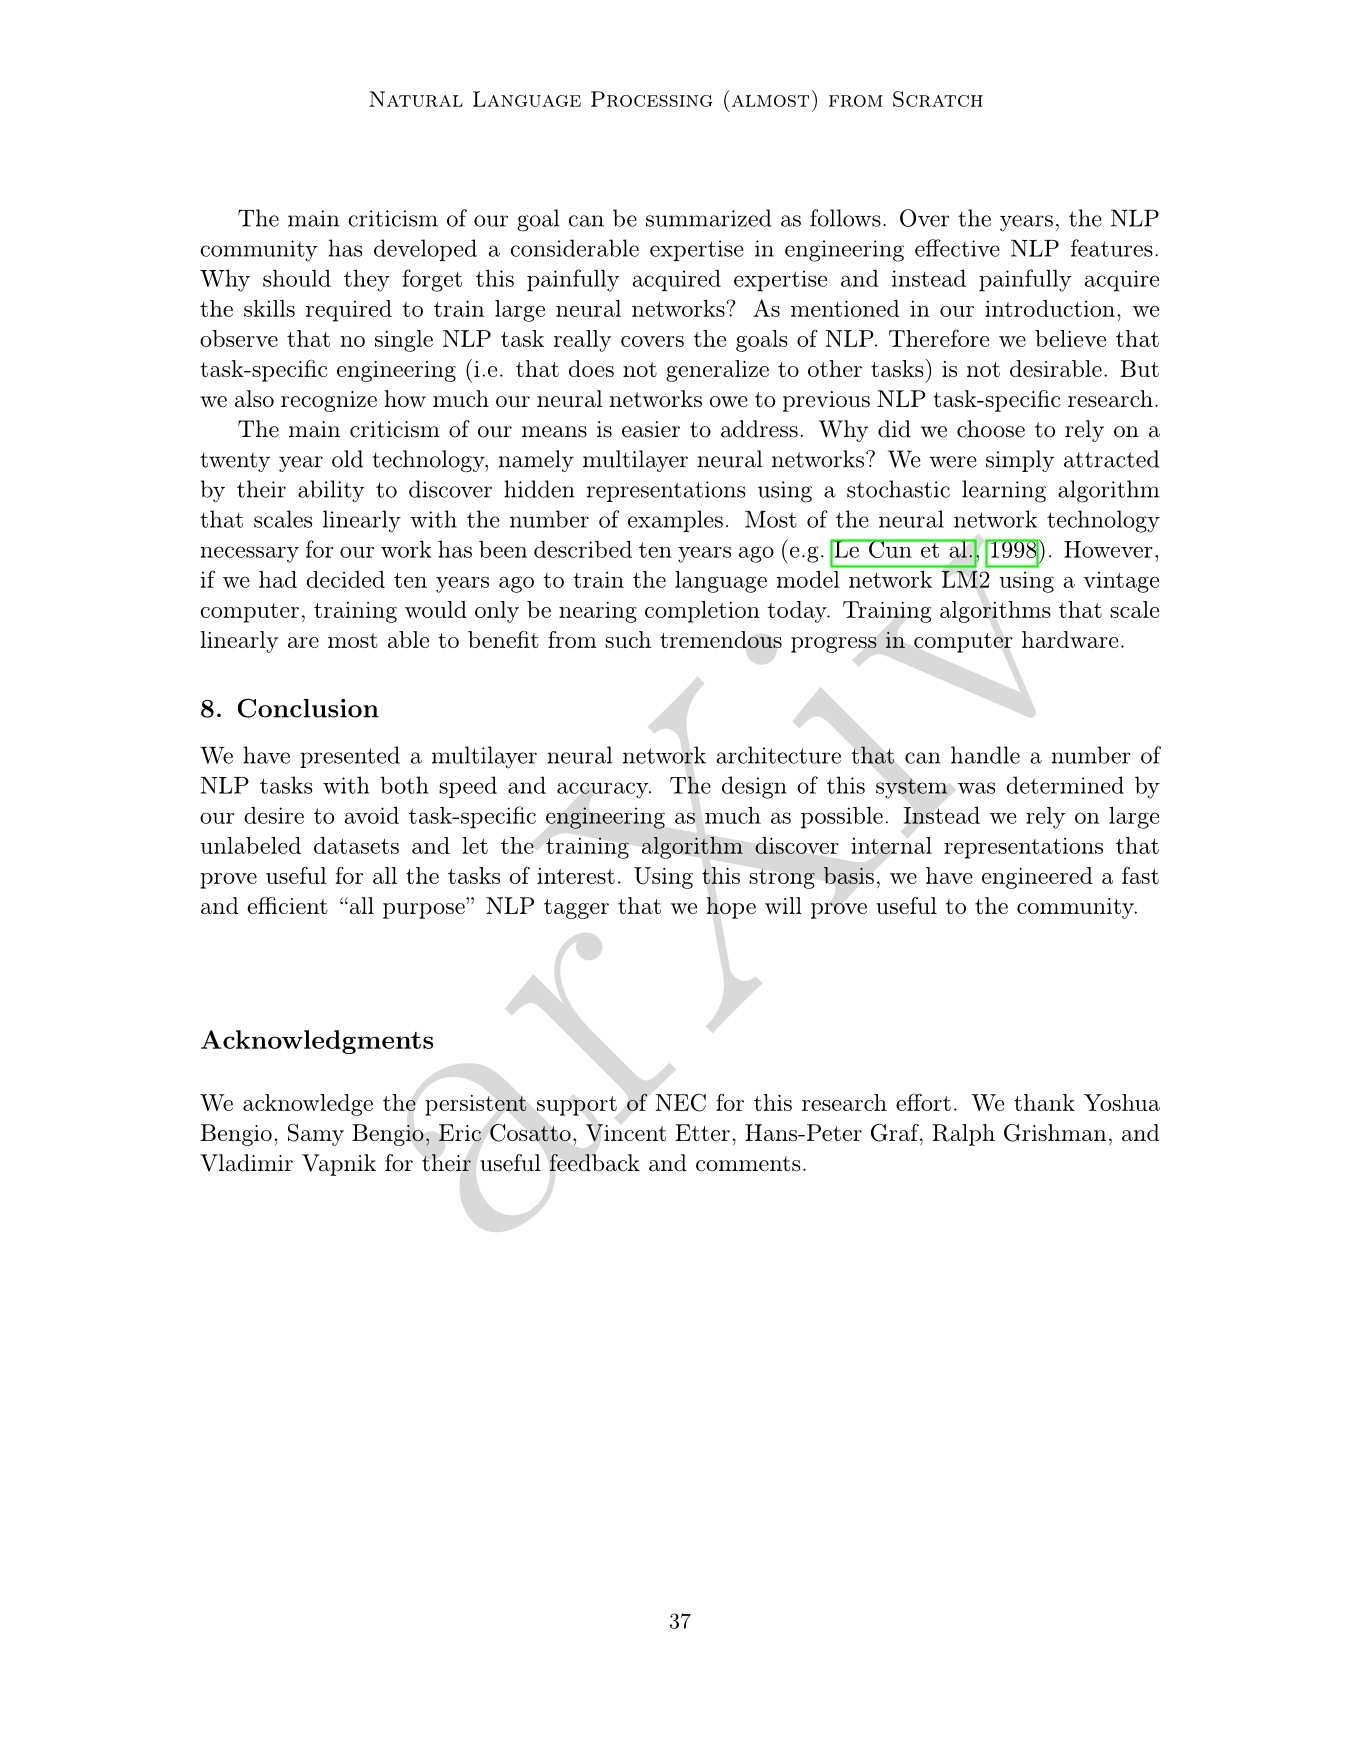
\includegraphics[width=\textwidth]{translations/collobert_2011-37.jpg}
\end{center}
\begin{center}
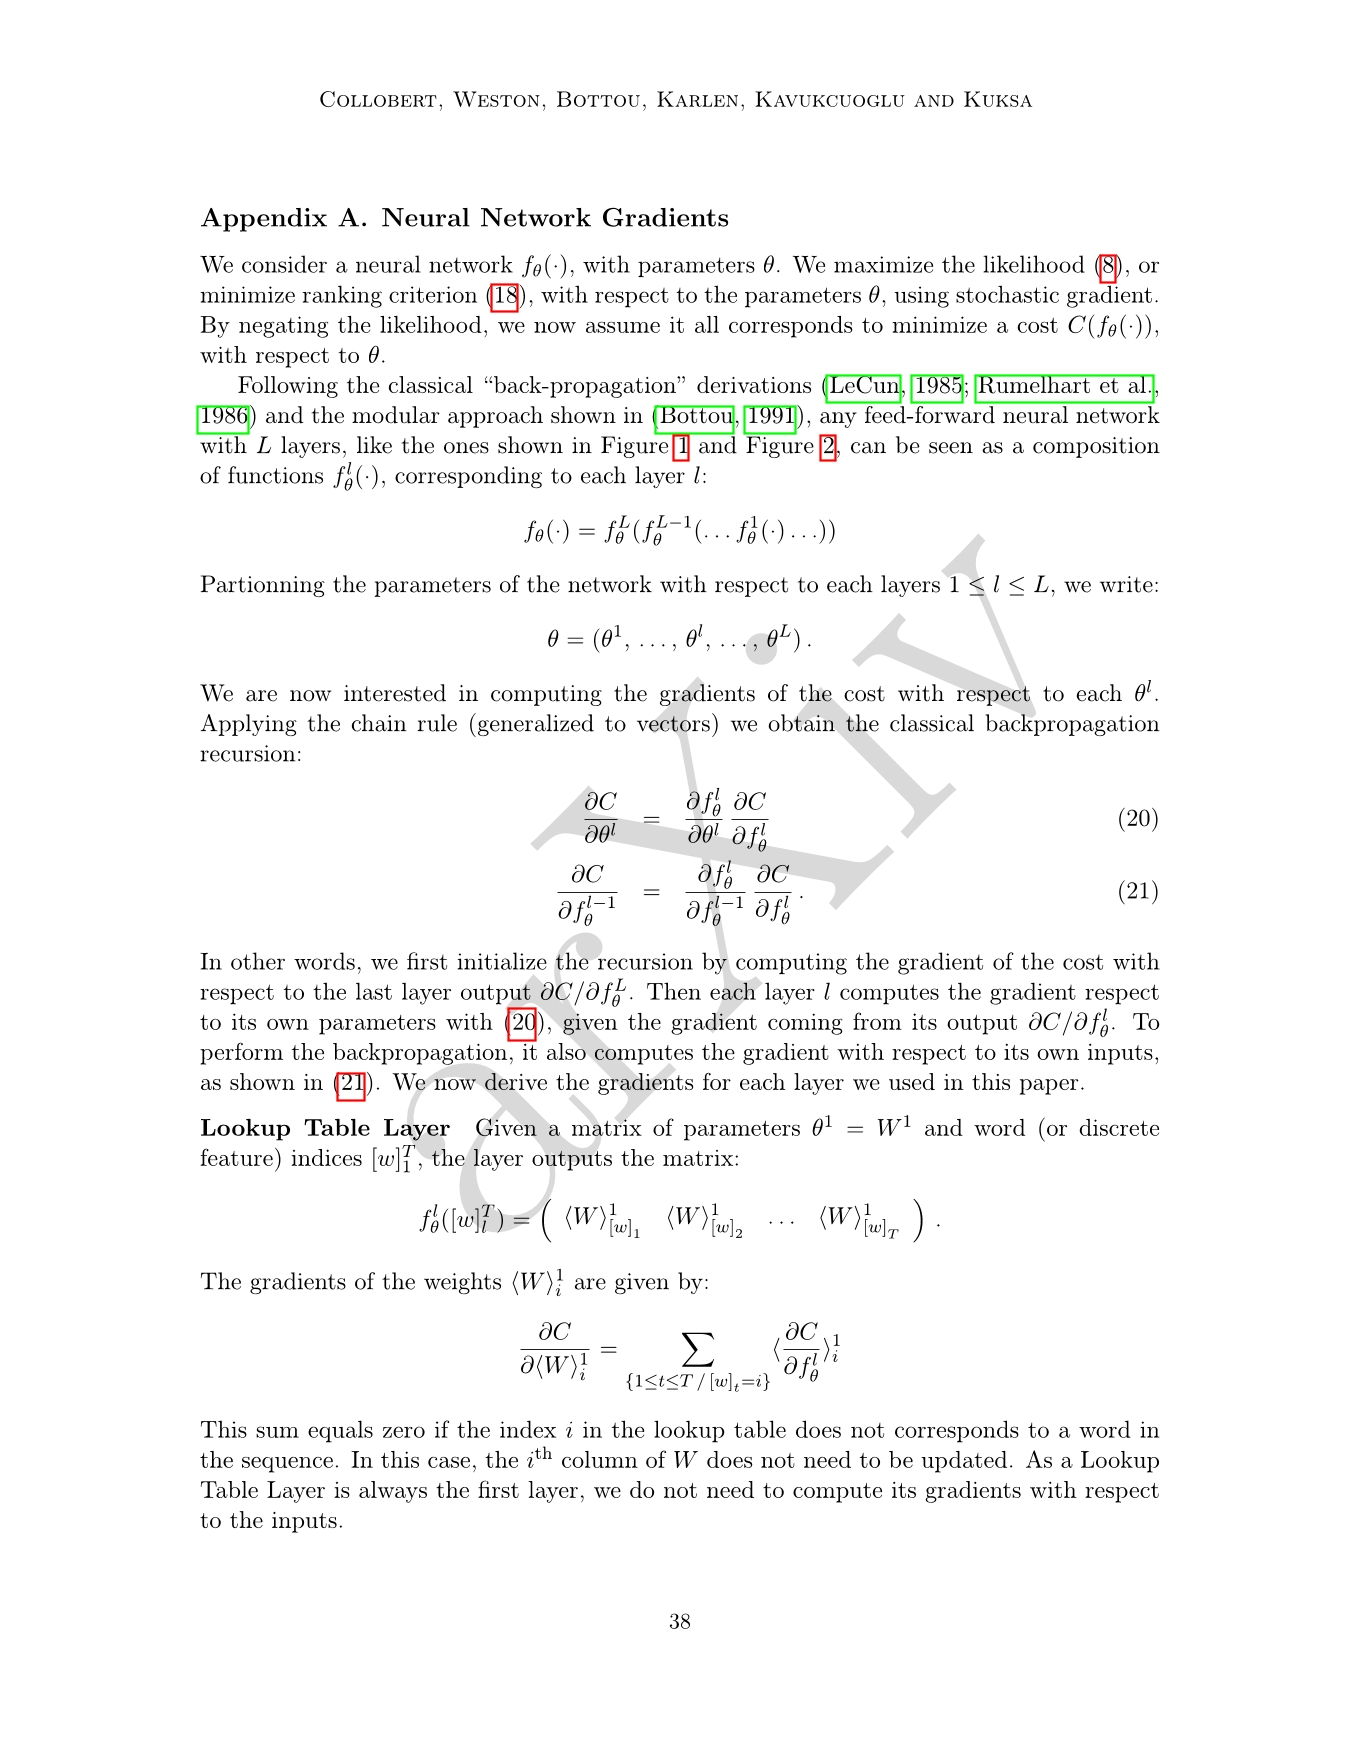
\includegraphics[width=\textwidth]{translations/collobert_2011-38.jpg}
\end{center}
\begin{center}
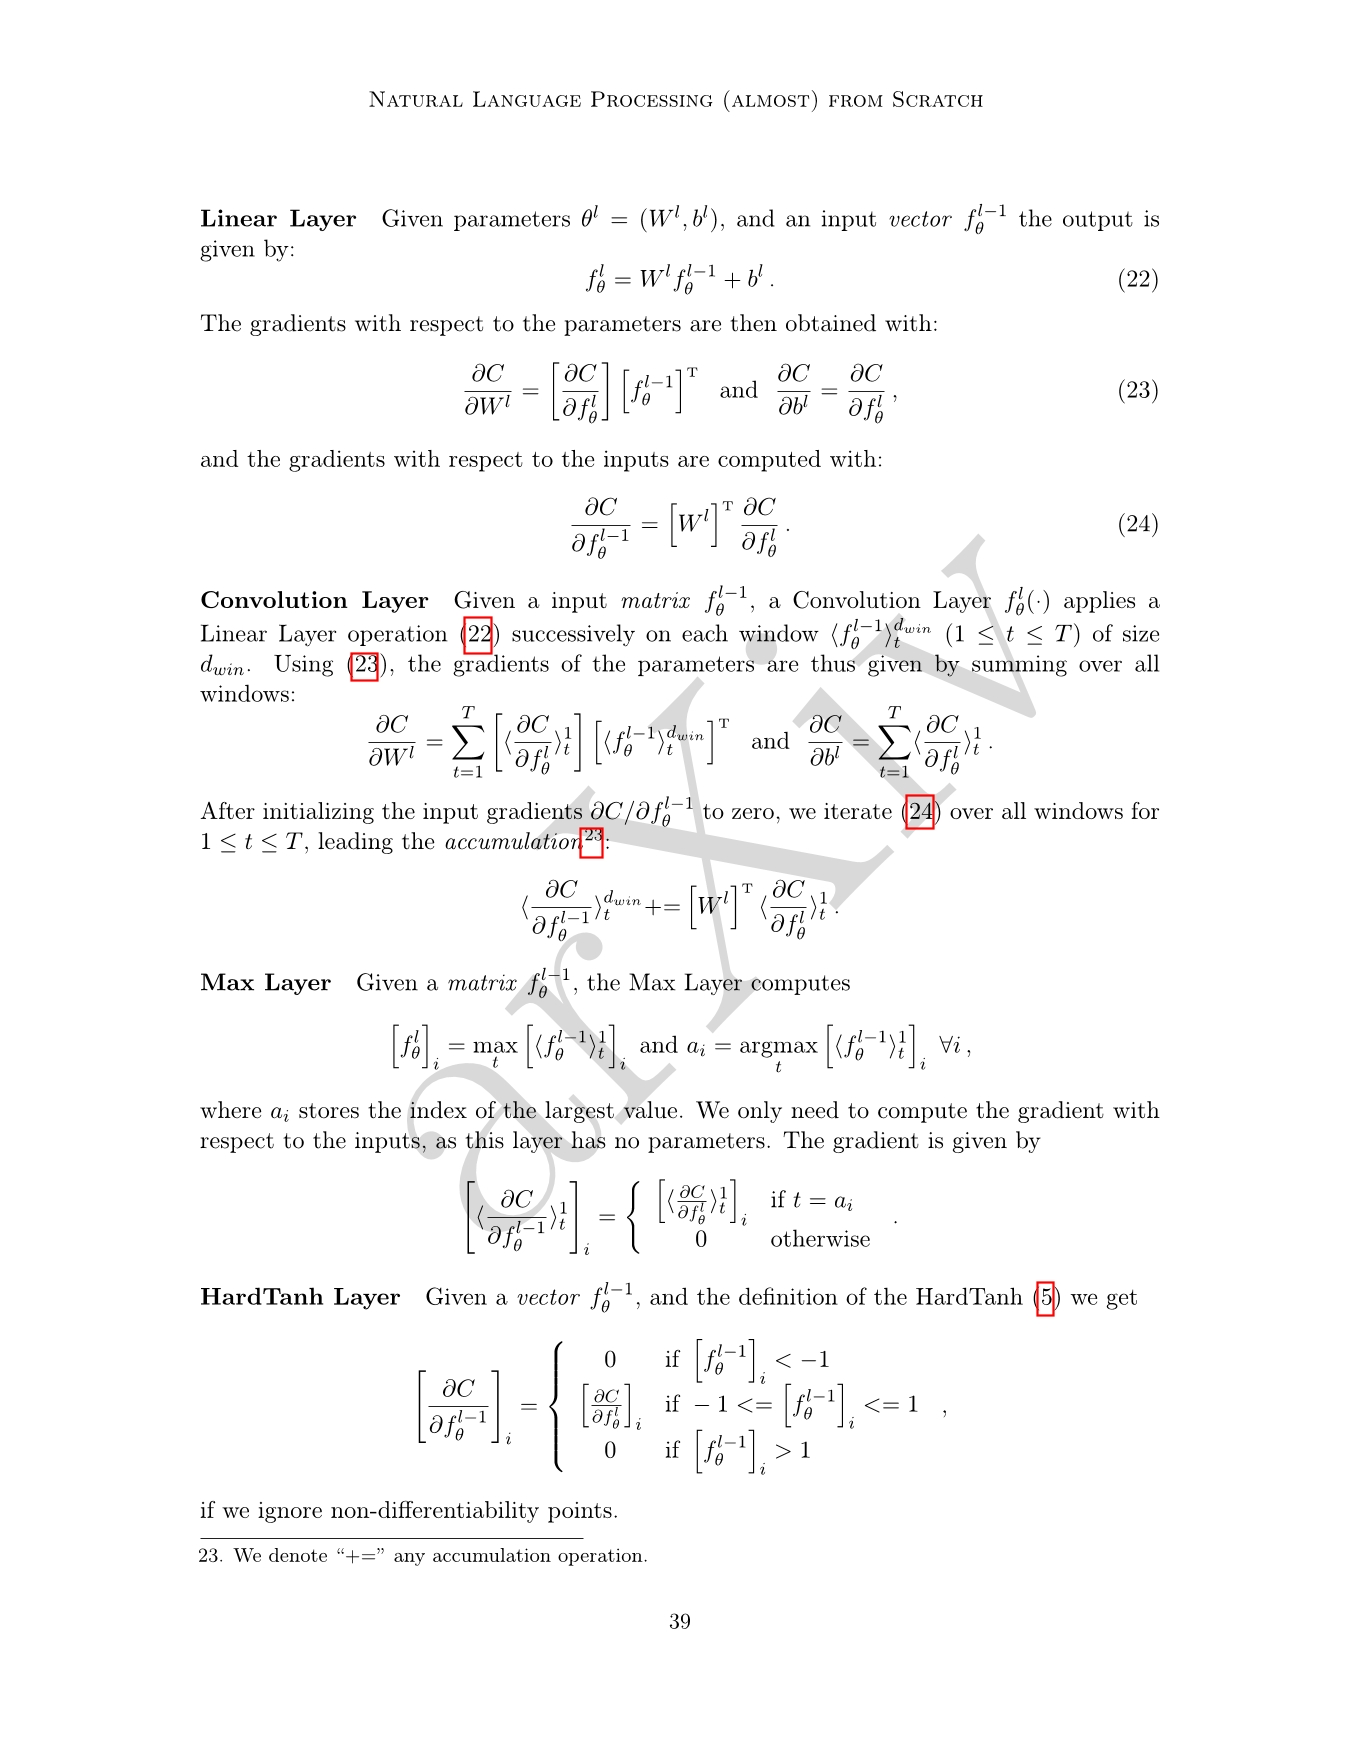
\includegraphics[width=\textwidth]{translations/collobert_2011-39.jpg}
\end{center}
\begin{center}
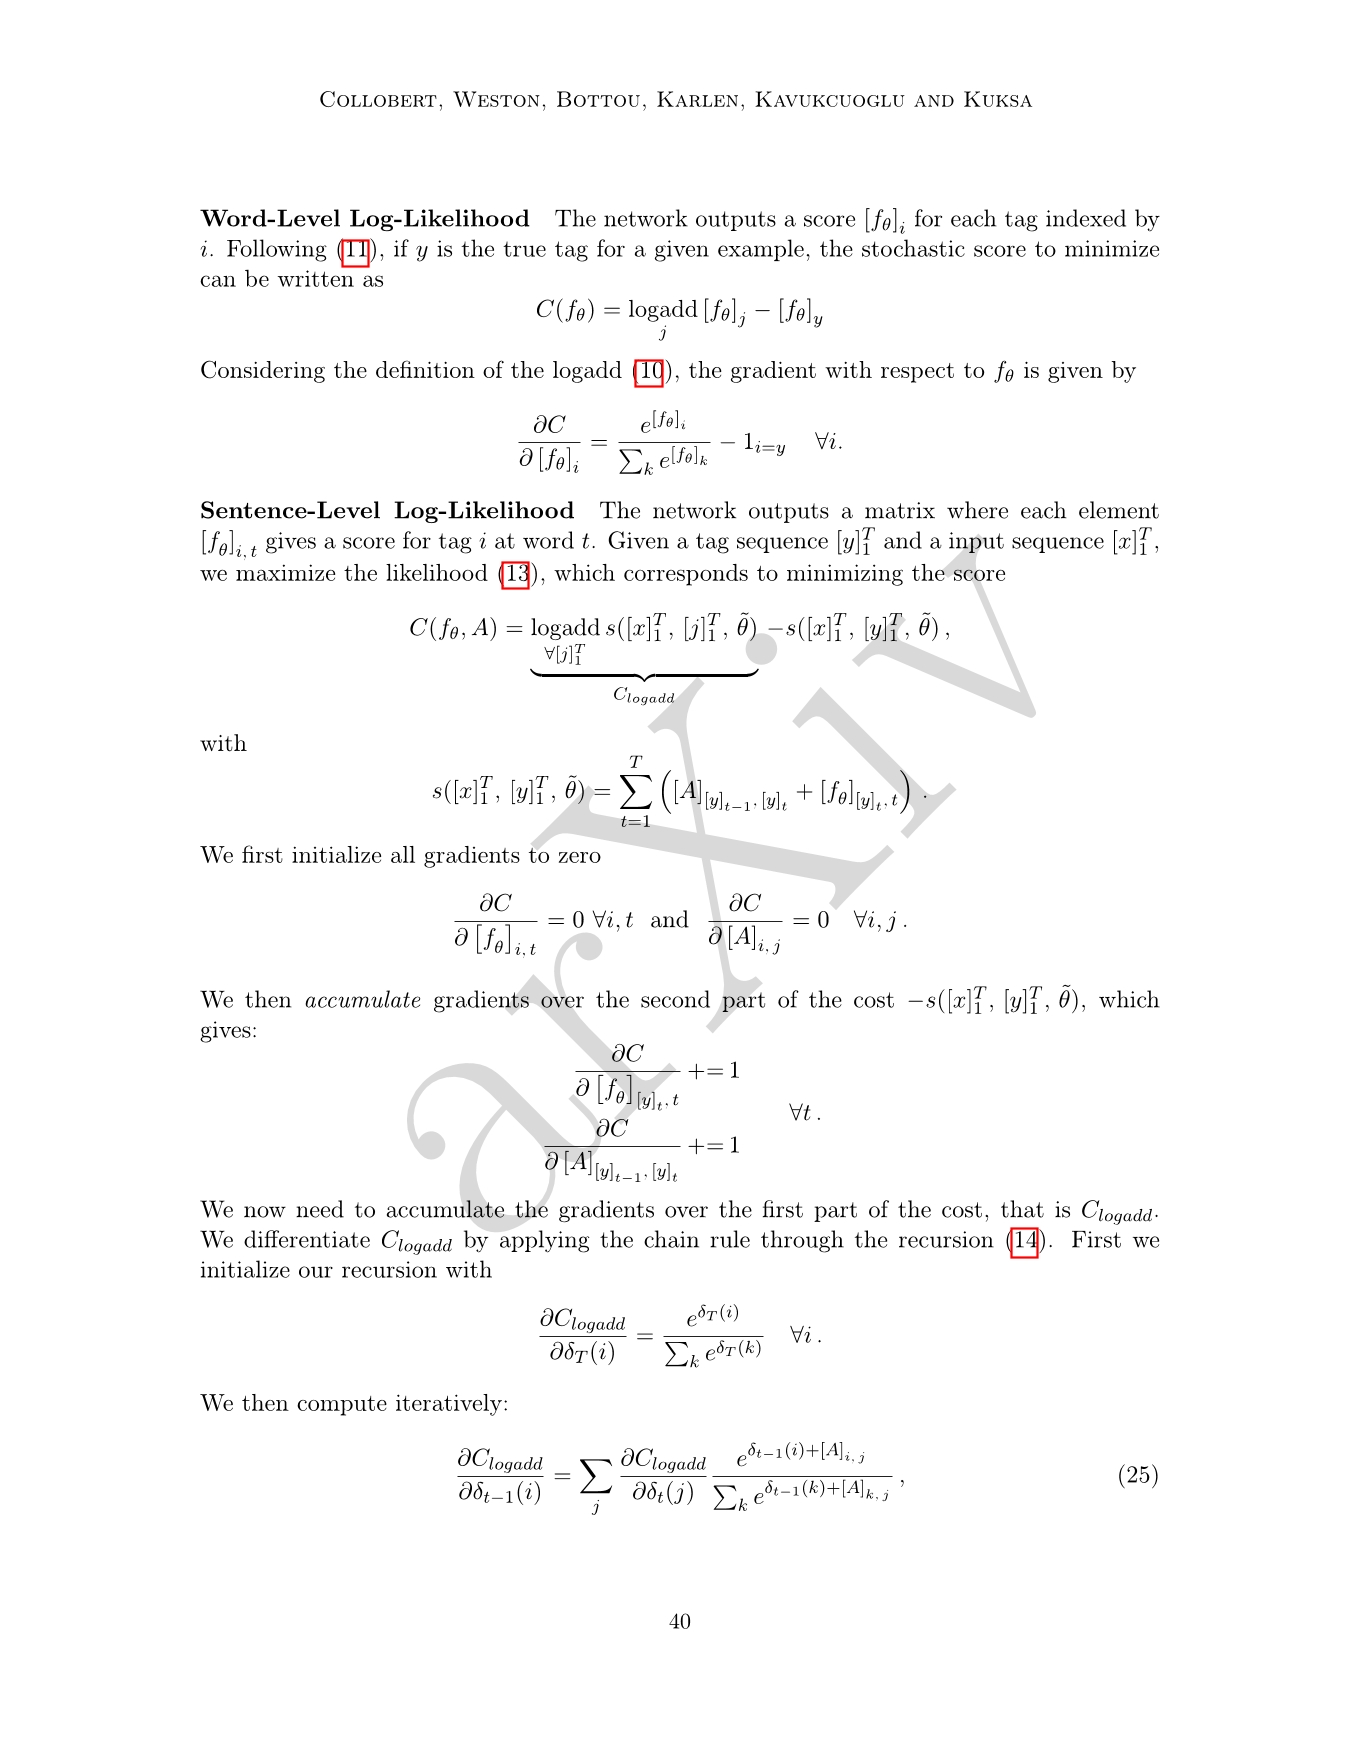
\includegraphics[width=\textwidth]{translations/collobert_2011-40.jpg}
\end{center}
\begin{center}
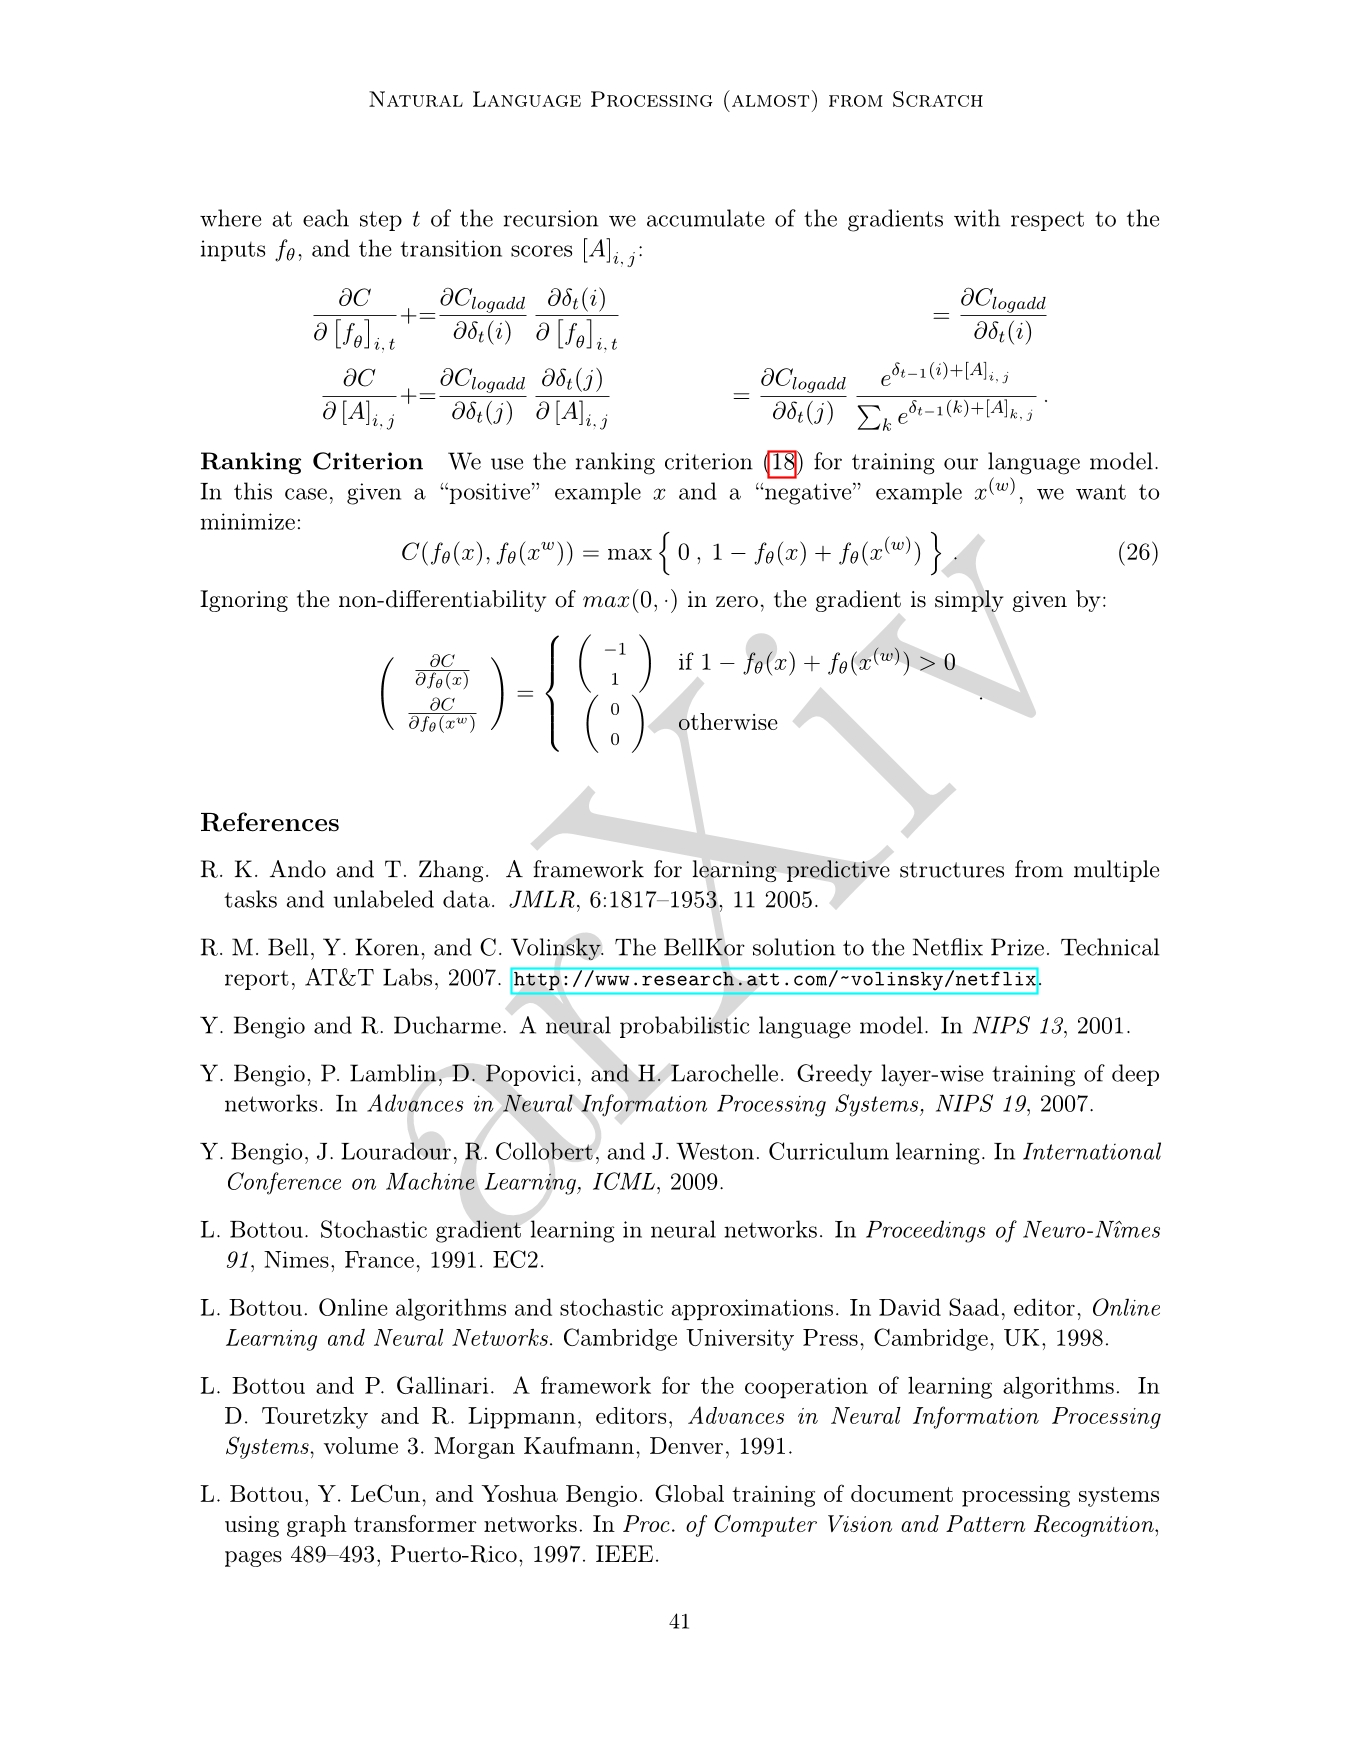
\includegraphics[width=\textwidth]{translations/collobert_2011-41.jpg}
\end{center}
\begin{center}
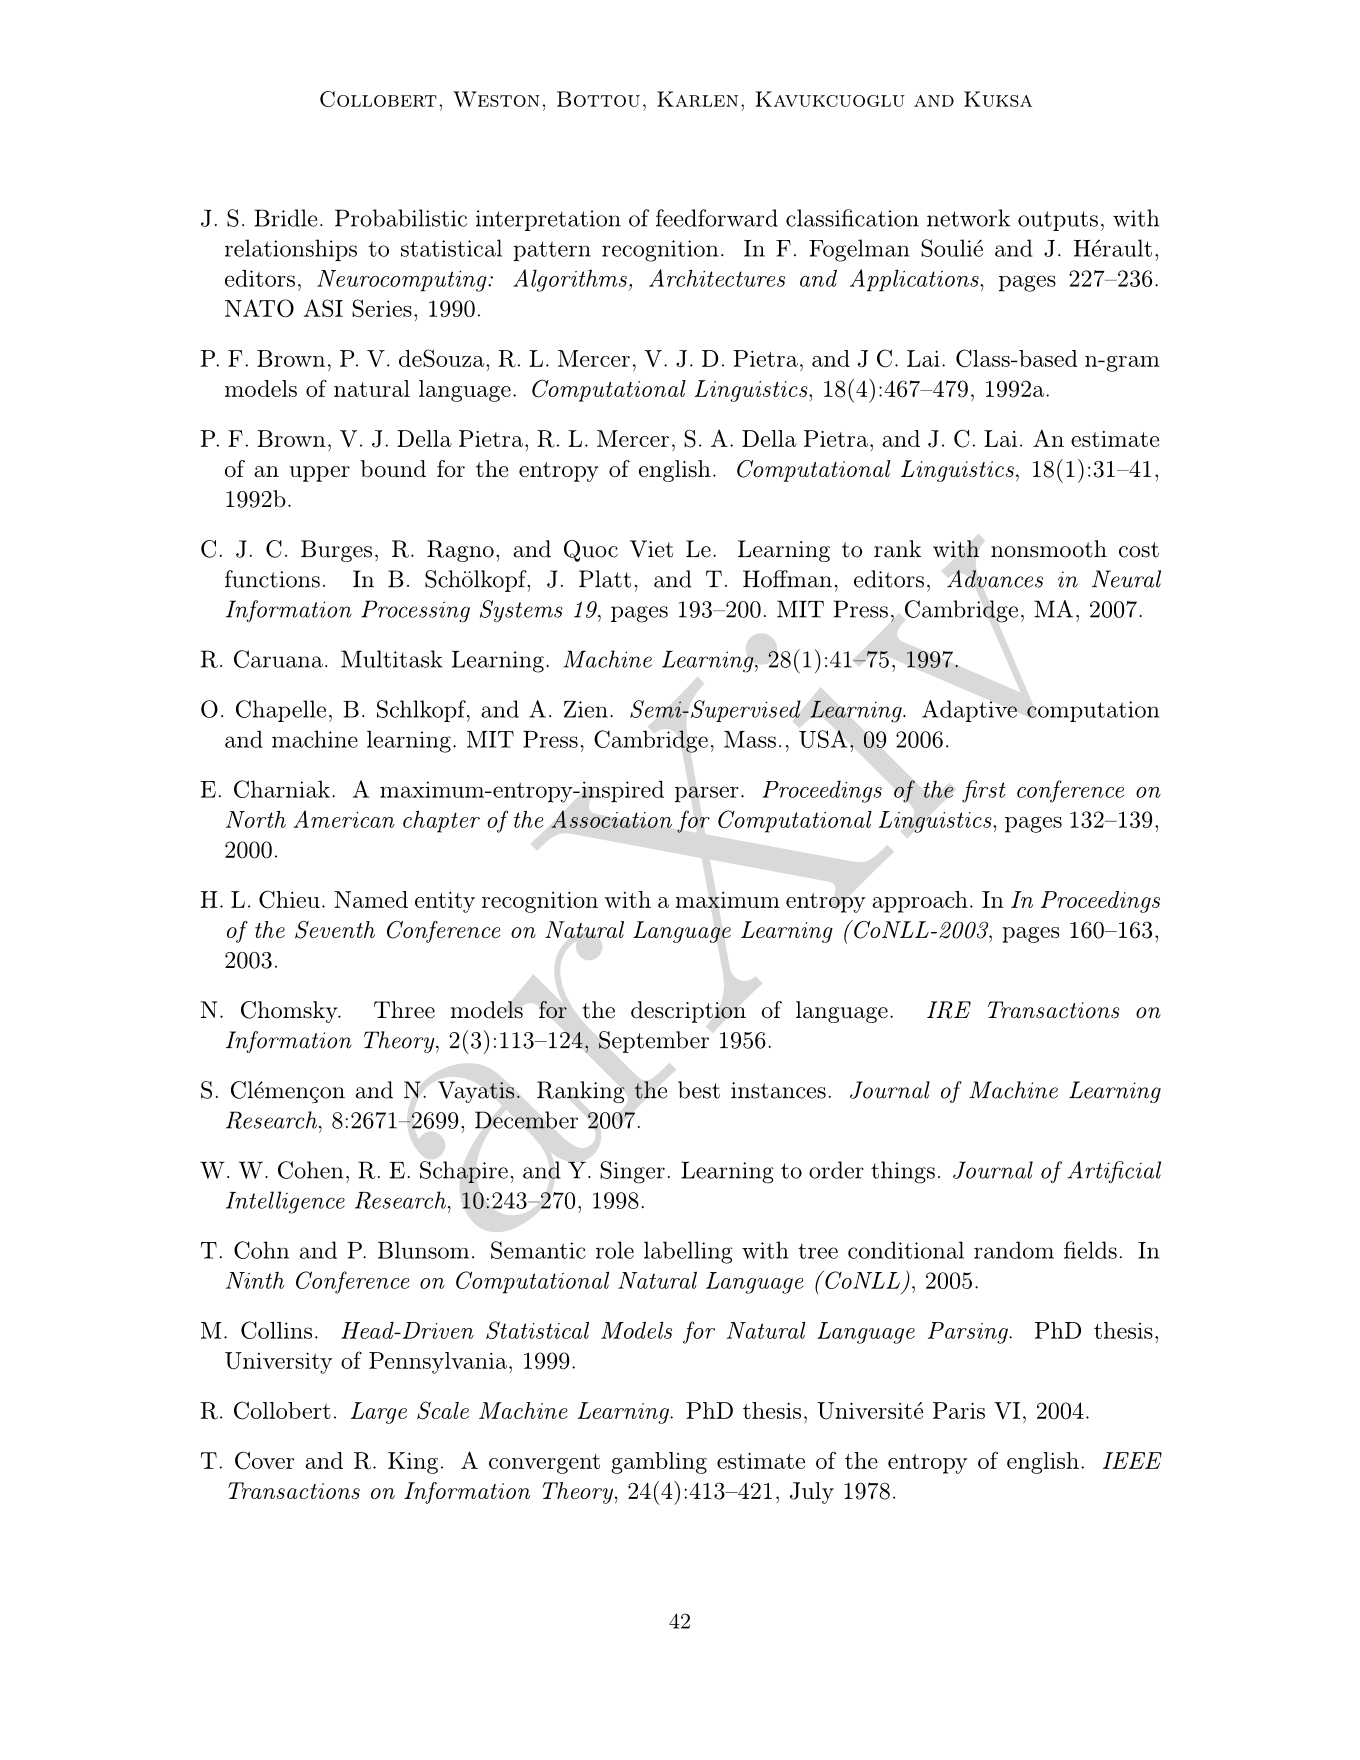
\includegraphics[width=\textwidth]{translations/collobert_2011-42.jpg}
\end{center}
\begin{center}
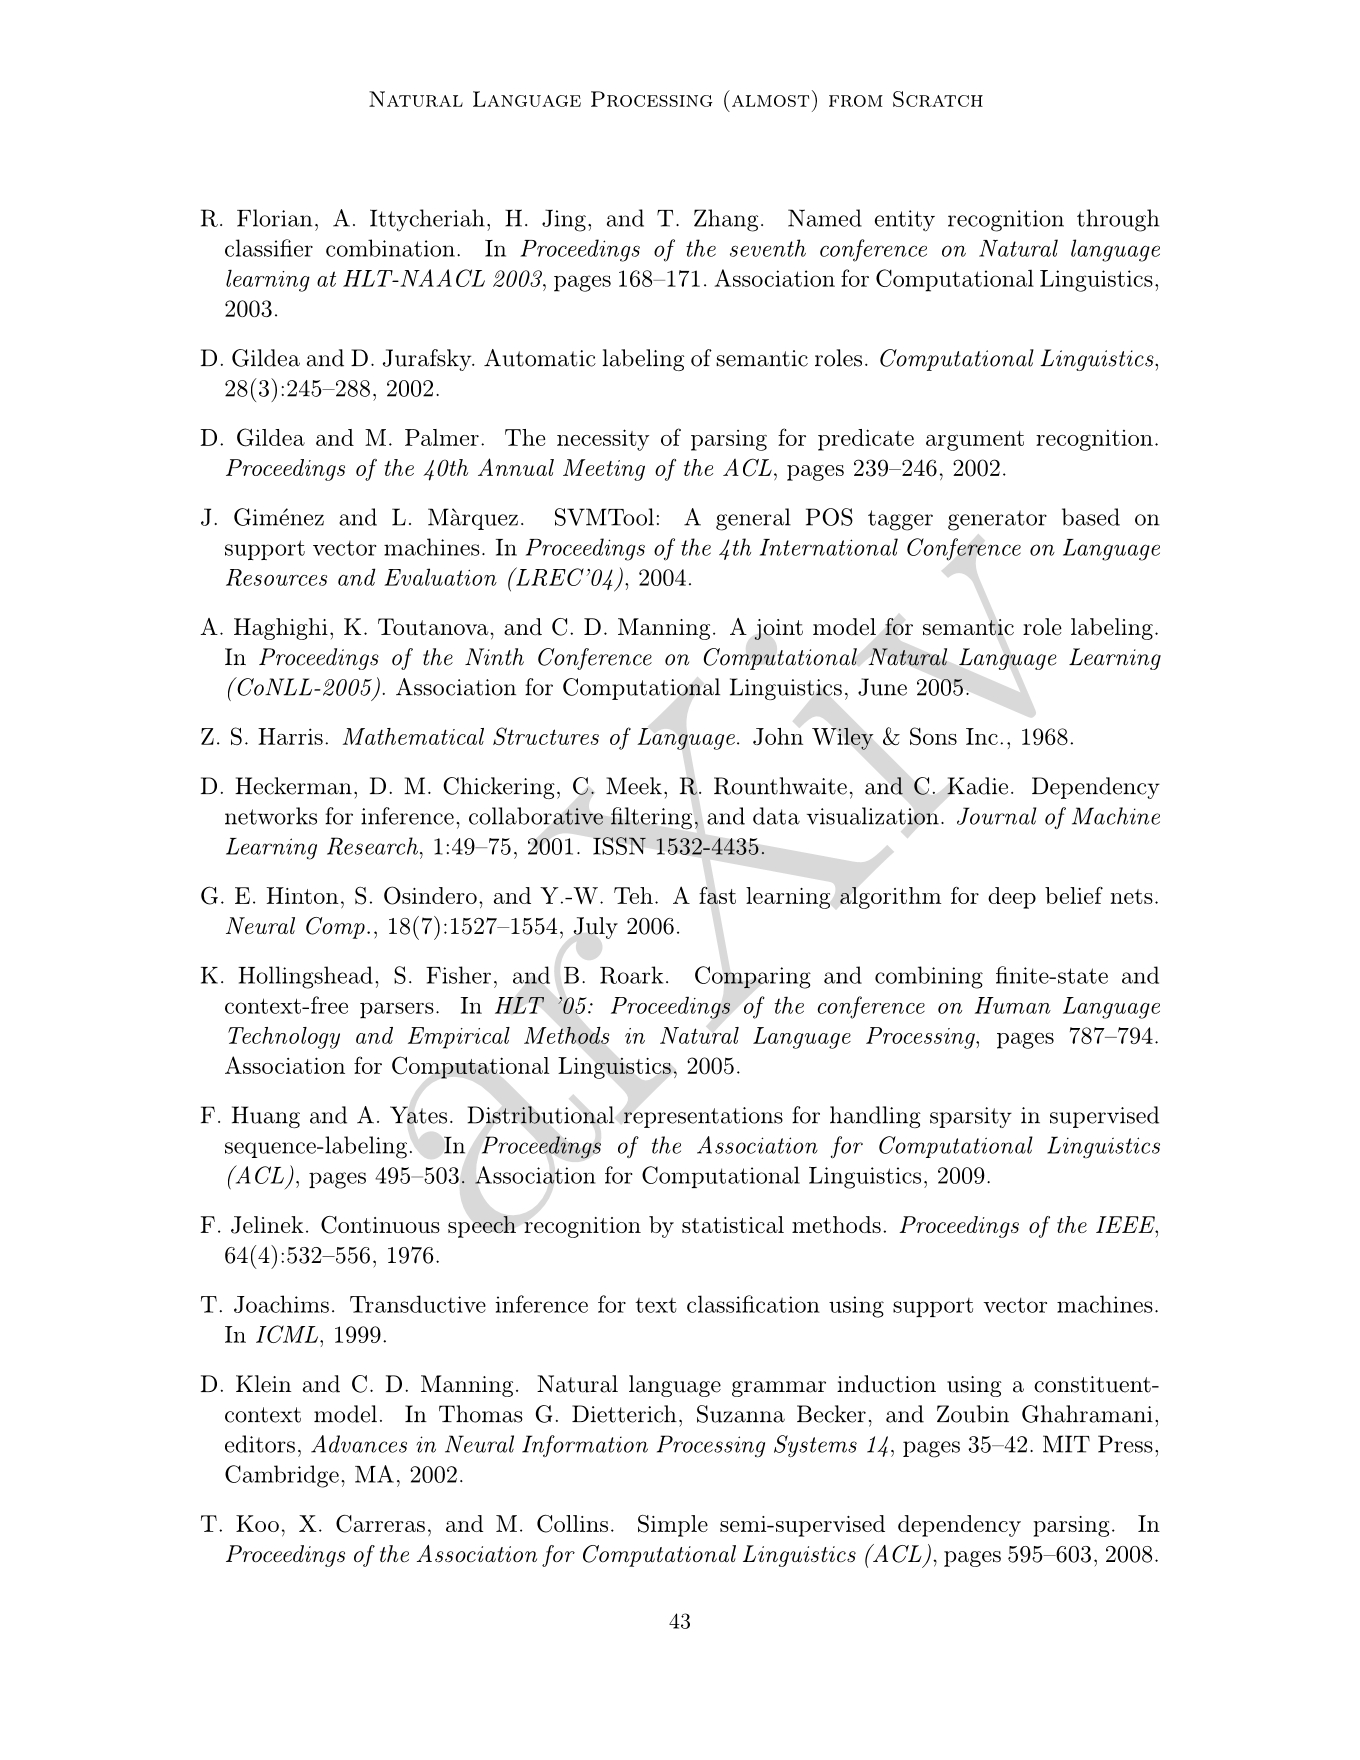
\includegraphics[width=\textwidth]{translations/collobert_2011-43.jpg}
\end{center}
\begin{center}
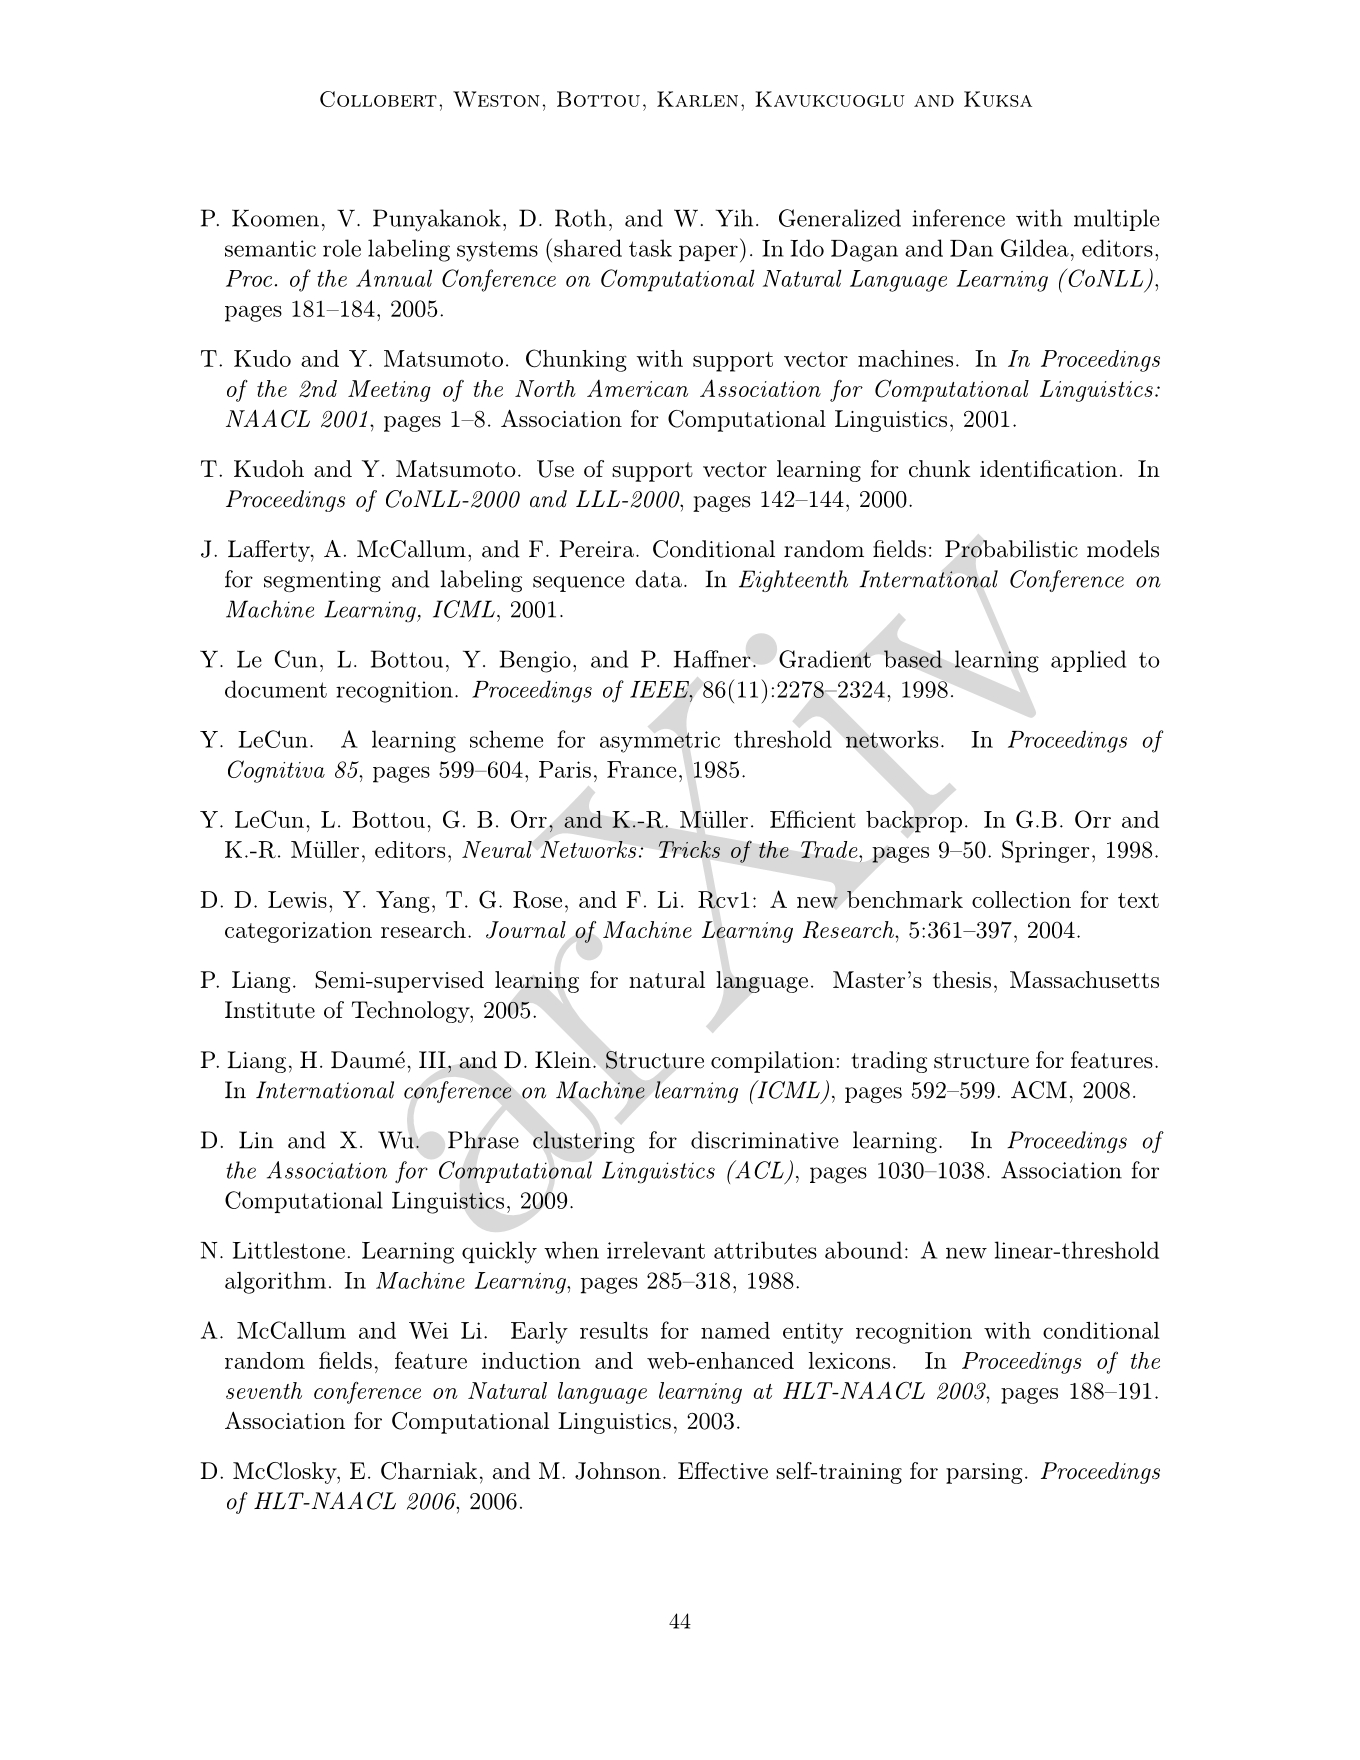
\includegraphics[width=\textwidth]{translations/collobert_2011-44.jpg}
\end{center}
\begin{center}
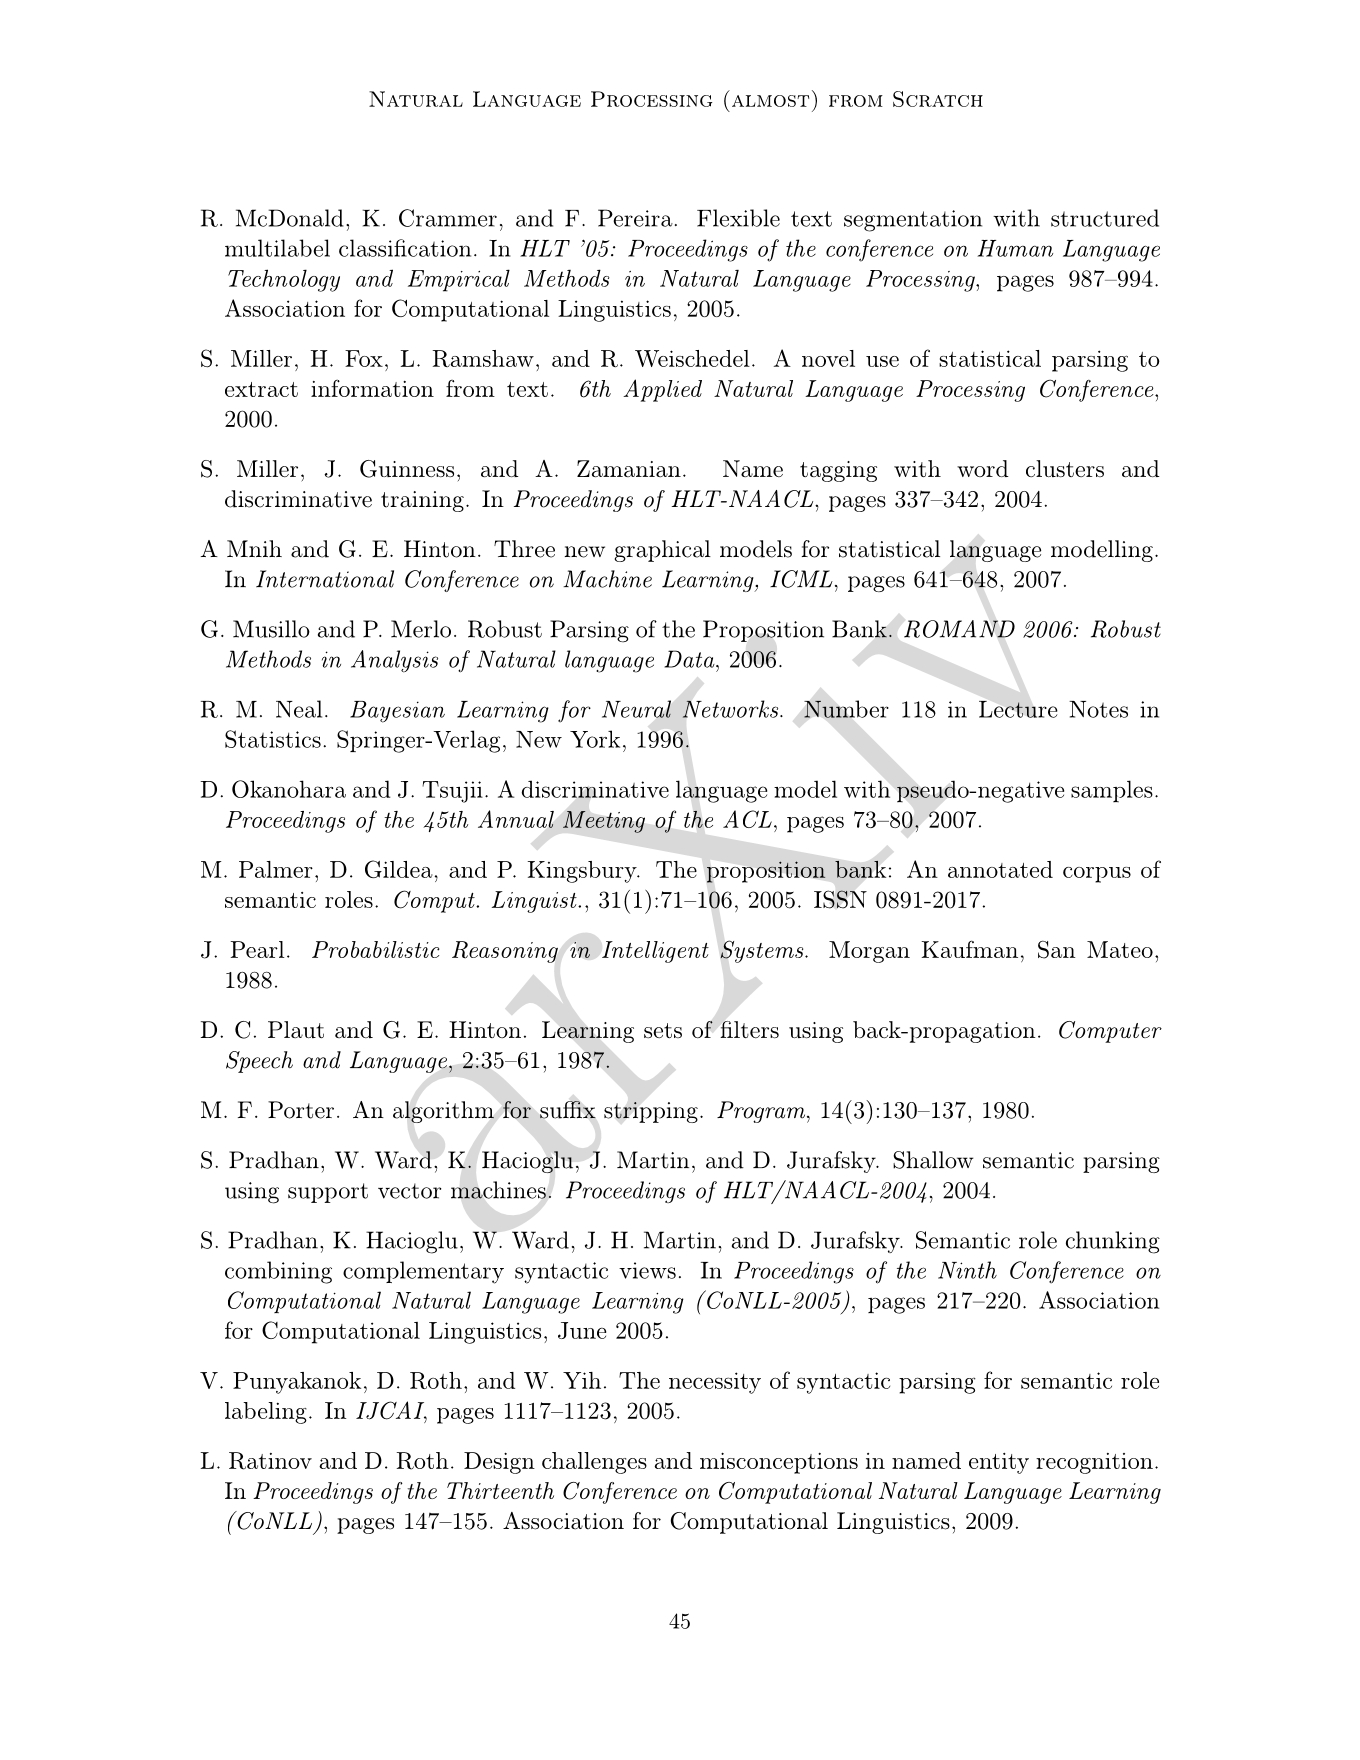
\includegraphics[width=\textwidth]{translations/collobert_2011-45.jpg}
\end{center}
\begin{center}
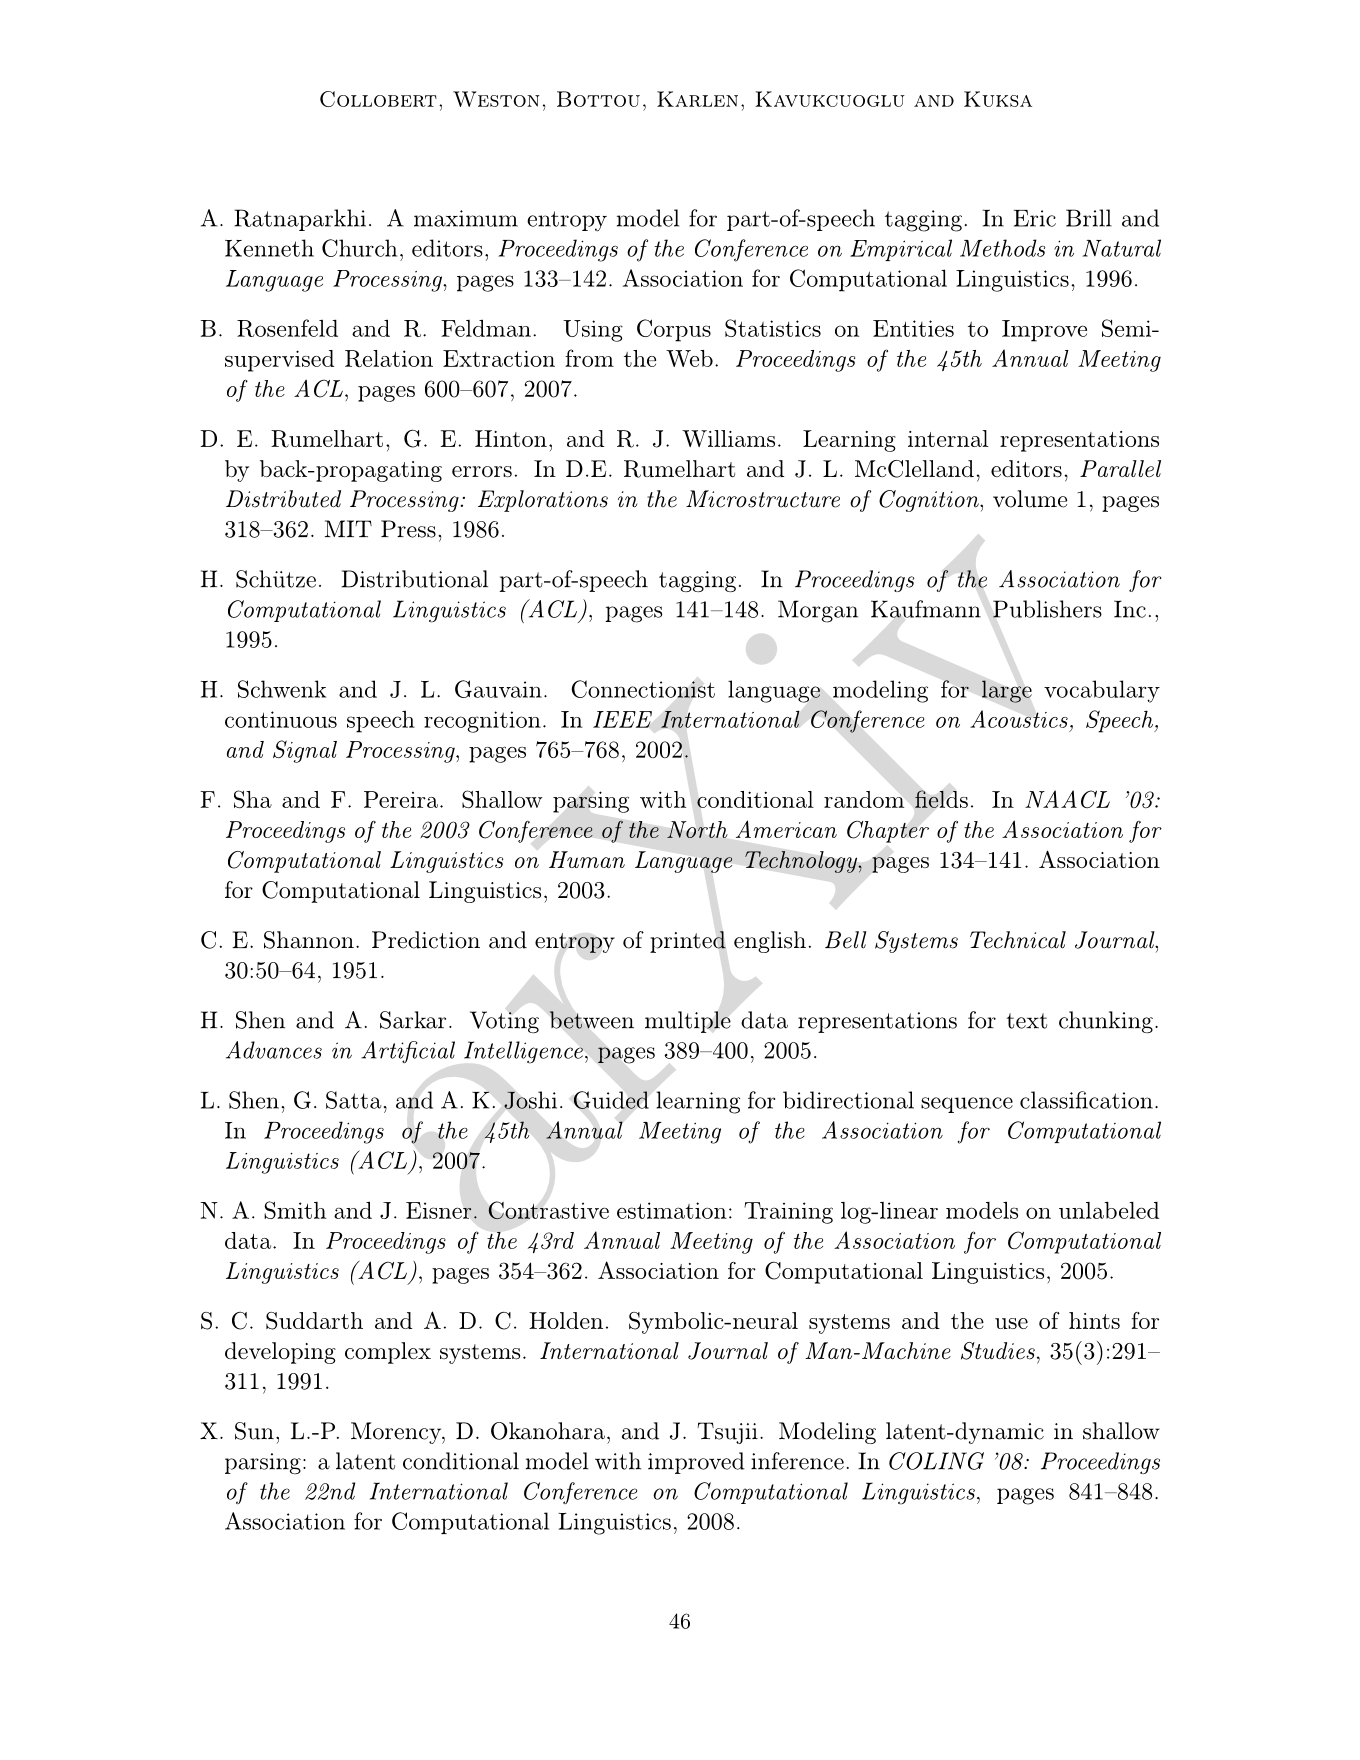
\includegraphics[width=\textwidth]{translations/collobert_2011-46.jpg}
\end{center}
\begin{center}
\includegraphics[width=\textwidth]{translations/collobert_2011-47.jpg}
\end{center}
